%
%               Template for sigplanconf LaTeX Class
%
% Name:         sigplanconf-template.tex
%
% Purpose:      A template for sigplanconf.cls, which is a LaTeX 2e class
%               file for SIGPLAN conference proceedings.
%
% Guide:        Refer to "Author's Guide to the ACM SIGPLAN Class,"
%               sigplanconf-guide.pdf
%
% Author:       Paul C. Anagnostopoulos
%               Windfall Software
%               978 371-2316
%               paul@windfall.com
%
% Created:      15 February 2005
%
%-----------------------------------------------------------------------------


\documentclass[10pt,reprint,nocopyrightspace,numbers]{sigplanconf}

% The following \documentclass options may be useful:

% preprint      Remove this option only once the paper is in final form.
% 10pt          To set in 10-point type instead of 9-point.
% 11pt          To set in 11-point type instead of 9-point.
% numbers       To obtain numeric citation style instead of author/year.

%\usepackage{amsmath}
\usepackage{mathptmx}
\usepackage{microtype}
%\usepackage{subfig}
\usepackage{bec}
\usepackage{tikz}
\usetikzlibrary{shapes,backgrounds,arrows,calc,automata,positioning}
\usepackage[underline=false]{pgf-umlsd}
%\usepackage{float}
\usepackage{paralist}
%\usepackage[subtle]{savetrees}

% Tikz directives for drawing HMM, PFSAs and other related macros
\newcommand\obs{
	\mathchoice
    	{{\scriptstyle\mathcal{O}}}% \displaystyle
    	{{\scriptstyle\mathcal{O}}}% \textstyle
    	{{\scriptscriptstyle\mathcal{O}}}% \scriptstyle
    	{\scalebox{.7}{$\scriptscriptstyle\mathcal{O}$}}%\scriptscriptstyle
}
\tikzstyle{hmmstate}=[shape=circle,draw=blue!50,fill=blue!20]
\tikzstyle{hmminitialabove}=[initial,initial text={$I_\mathcal{H}:1$}, initial where=above]
\tikzstyle{hmminitialleft}=[initial,initial text={$I_\mathcal{H}:1$}, initial where=left]
\tikzstyle{hmminitialright}=[initial,initial text={$I_\mathcal{H}:1$}, initial where=right]
\tikzstyle{pfsainitial}=[initial,initial text={$I(x_1):1$}, initial where=above]
\tikzstyle{pfsainitialabove}=[initial,initial text={$I_\mathcal{A}:1$}, initial where=above]
\tikzstyle{pfsainitialleft}=[initial,initial text={$I_\mathcal{A}:1$}, initial where=left]
\tikzstyle{pfsainitialright}=[initial,initial text={$I_\mathcal{A}:1$}, initial where=right]
\tikzstyle{pfsafinal}=[hmmstate,accepting]
\tikzstyle{observation}=[shape=rectangle,draw=orange!50,fill=orange!20]
\tikzstyle{lightedge}=[<-,dotted]
\tikzstyle{mainstate}=[state,thick]
\tikzstyle{mainedge}=[<-,thick]

%\newcommand{\cL}{{\cal L}}

% eliminate orphans and widows
%\clubpenalty = 10000
%\widowpenalty = 10000
%\displaywidowpenalty = 10000

% Make it easier for a figure and text to share a column.
\renewcommand{\topfraction}{0.95}
\renewcommand{\textfraction}{0.05}
\renewcommand{\floatpagefraction}{0.9}

%%%
%%% Show/Hide Comments
%%%
%\setboolean{showcomments}{false}
\setboolean{showjedi}{false}

\begin{document}
%TODO
\newcommand{\todo}[1]{{\color{red}{\bf [TODO]:~{#1}}}}

%THEOREMS
\newtheorem{theorem}{Theorem}
\newtheorem{corollary}{Corollary}
\newtheorem{lemma}{Lemma}
\newtheorem{proposition}{Proposition}
\newtheorem{problem}{Problem}
\newtheorem{definition}{Definition}
\newtheorem{remark}{Remark}
\newtheorem{example}{Example}
\newtheorem{assumption}{Assumption}

%HANS' CONVENIENCES
\newcommand{\define}[1]{\textit{#1}}
\newcommand{\join}{\vee}
\newcommand{\meet}{\wedge}
\newcommand{\bigjoin}{\bigvee}
\newcommand{\bigmeet}{\bigwedge}
\newcommand{\jointimes}{\boxplus}
\newcommand{\meettimes}{\boxplus'}
\newcommand{\bigjoinplus}{\bigjoin}
\newcommand{\bigmeetplus}{\bigmeet}
\newcommand{\joinplus}{\join}
\newcommand{\meetplus}{\meet}
\newcommand{\lattice}[1]{\mathbf{#1}}
\newcommand{\semimod}{\mathcal{S}}
\newcommand{\graph}{\mathcal{G}}
\newcommand{\nodes}{\mathcal{V}}
\newcommand{\agents}{\{1,2,\dots,N\}}
\newcommand{\edges}{\mathcal{E}}
\newcommand{\neighbors}{\mathcal{N}}
\newcommand{\Weights}{\mathcal{A}}
\renewcommand{\leq}{\leqslant}
\renewcommand{\geq}{\geqslant}
\renewcommand{\preceq}{\preccurlyeq}
\renewcommand{\succeq}{\succcurlyeq}
\newcommand{\Rmax}{\mathbb{R}_{\mathrm{max}}}
\newcommand{\Rmin}{\mathbb{R}_{\mathrm{min}}}
\newcommand{\Rext}{\overline{\mathbb{R}}}
\newcommand{\R}{\mathbb{R}}
\newcommand{\N}{\mathbb{N}}
\newcommand{\A}{\mathbf{A}}
\newcommand{\B}{\mathbf{B}}
\newcommand{\x}{\mathbf{x}}
\newcommand{\e}{\mathbf{e}}
\newcommand{\X}{\mathbf{X}}
\newcommand{\W}{\mathbf{W}}
\newcommand{\weights}{\mathcal{W}}
\newcommand{\alternatives}{\mathcal{X}}
\newcommand{\xsol}{\bar{\mathbf{x}}}
\newcommand{\y}{\mathbf{y}}
\newcommand{\Y}{\mathbf{Y}}
\newcommand{\z}{\mathbf{z}}
\newcommand{\Z}{\mathbf{Z}}
\renewcommand{\a}{\mathbf{a}}
\renewcommand{\b}{\mathbf{b}}
\newcommand{\I}{\mathbf{I}}
\DeclareMathOperator{\supp}{supp}
\newcommand{\Par}[2]{\mathcal{P}_{{#1} \to {#2}}}
\newcommand{\Laplacian}{\mathcal{L}}
\newcommand{\F}{\mathcal{F}}
\newcommand{\inv}[1]{{#1}^{\sharp}}
\newcommand{\energy}{Q}
\newcommand{\err}{\mathrm{err}}
\newcommand{\argmin}{\mathrm{argmin}}
\newcommand{\argmax}{\mathrm{argmax}}


\special{papersize=8.5in,11in}
\setlength{\pdfpageheight}{\paperheight}
\setlength{\pdfpagewidth}{\paperwidth}

\conferenceinfo{CONF 'yy}{Month d--d, 20yy, City, ST, Country}
\copyrightyear{20yy}
\copyrightdata{978-1-nnnn-nnnn-n/yy/mm}
\copyrightdoi{nnnnnnn.nnnnnnn}

% Uncomment the publication rights you want to use.
%\publicationrights{transferred}
%\publicationrights{licensed}     % this is the default
%\publicationrights{author-pays}

%\titlebanner{banner above paper title}        % These are ignored unless
%\preprintfooter{short description of paper}   % 'preprint' option specified.

\title{Abstracting Event-Driven Systems with Lifestate Rules}
%\subtitle{Subtitle Text, if any}

\authorinfo{Shawn Meier
\and Aleksandar Chakarov
\and Maxwell Russek
\\ Sergio Mover
\and Bor-Yuh Evan Chang%
}
           {University of Colorado Boulder}
           {\{shawn.meier, aleksandar.chakarov, maxwell.russek, sergio.mover, evan.chang\}@colorado.edu}
%\authorinfo{Name2\and Name3}
%           {Affiliation2/3}
%           {Email2/3}

\maketitle

\begin{abstract}
  In this paper, we explore the connection between secret key agreement and secure omniscience within the setting of the multiterminal source model with a wiretapper who has side information. While the secret key agreement problem considers the generation of a maximum-rate secret key through public discussion, the secure omniscience problem is concerned with communication protocols for omniscience that minimize the rate of information leakage to the wiretapper. The starting point of our work is a lower bound on the minimum leakage rate for omniscience, $\rl$, in terms of the wiretap secret key capacity, $\wskc$. Our interest is in identifying broad classes of sources for which this lower bound is met with equality, in which case we say that there is a duality between secure omniscience and secret key agreement. We show that this duality holds in the case of certain finite linear source (FLS) models, such as two-terminal FLS models and pairwise independent network models on trees with a linear wiretapper. Duality also holds for any FLS model in which $\wskc$ is achieved by a perfect linear secret key agreement scheme. We conjecture that the duality in fact holds unconditionally for any FLS model. On the negative side, we give an example of a (non-FLS) source model for which duality does not hold if we limit ourselves to communication-for-omniscience protocols with at most two (interactive) communications.  We also address the secure function computation problem and explore the connection between the minimum leakage rate for computing a function and the wiretap secret key capacity.
  
%   Finally, we demonstrate the usefulness of our lower bound on $\rl$ by using it to derive equivalent conditions for the positivity of $\wskc$ in the multiterminal model. This extends a recent result of Gohari, G\"{u}nl\"{u} and Kramer (2020) obtained for the two-user setting.
  
   
%   In this paper, we study the problem of secret key generation through an omniscience achieving communication that minimizes the 
%   leakage rate to a wiretapper who has side information in the setting of multiterminal source model.  We explore this problem by deriving a lower bound on the wiretap secret key capacity $\wskc$ in terms of the minimum leakage rate for omniscience, $\rl$. 
%   %The former quantity is defined to be the maximum secret key rate achievable, and the latter one is defined as the minimum possible leakage rate about the source through an omniscience scheme to a wiretapper. 
%   The main focus of our work is the characterization of the sources for which the lower bound holds with equality \textemdash it is referred to as a duality between secure omniscience and wiretap secret key agreement. For general source models, we show that duality need not hold if we limit to the communication protocols with at most two (interactive) communications. In the case when there is no restriction on the number of communications, whether the duality holds or not is still unknown. However, we resolve this question affirmatively for two-user finite linear sources (FLS) and pairwise independent networks (PIN) defined on trees, a subclass of FLS. Moreover, for these sources, we give a single-letter expression for $\wskc$. Furthermore, in the direction of proving the conjecture that duality holds for all FLS, we show that if $\wskc$ is achieved by a \emph{perfect} secret key agreement scheme for FLS then the duality must hold. All these results mount up the evidence in favor of the conjecture on FLS. Moreover, we demonstrate the usefulness of our lower bound on $\wskc$ in terms of $\rl$ by deriving some equivalent conditions on the positivity of secret key capacity for multiterminal source model. Our result indeed extends the work of Gohari, G\"{u}nl\"{u} and Kramer in two-user case.
\end{abstract}

%\category{CR-number}{subcategory}{third-level}

% general terms are not compulsory anymore,
% you may leave them out
%\terms
%term1, term2

%\keywords
%keyword1, keyword2

\section{Introduction}
\label{sec:introduction}


\JEDI{Motivation: Challenge in developing against event-driven frameworks.}
We consider the problem of specifying and mining the object protocols used by event-driven software frameworks.
Programming against event-driven frameworks is hard. 
In such frameworks, programmers develop client applications~(\emph{apps}) against the \emph{framework} by implementing \emph{callback} interfaces that enable the application to be notified when an \emph{event} managed by the framework occurs (e.g., a user-interface~(UI) button is pressed). The app may then delegate back to the framework through method calls to the application programming interface~(API) (e.g., to direct a change in the UI display).
To develop working apps, the application programmer must understand the complex object protocols implemented by the event-driven framework. For example, the framework may guarantee particular ordering constraints on callback invocations (known as \emph{lifecycle} constraints), and the application programmer may have to respect particular orderings of API calls (i.e., \emph{typestate} constraints%~\cite{strom+1986:typestate:-programming}
).

\JEDI{Why important: Such frameworks are pervasive. Why hard: No specs about these constraints. Hard to get because of size of framework and native code.}
%Formal reasoning about apps has become increasingly important due to the pervasive use of event-driven frameworks in creating mobile and web applications (e.g., Android, iOS, Node.js, DOM).
Unfortunately, such protocol specifications are complex to describe and maintain---and almost always incomplete. Because lifecycle constraints are so central to implementing apps, they are typically discussed in the framework documentation,
%(e.g., \cite{android-activities, iosuikit-uiview, emberjs-lifecycle, react-lifecycle}),
but they are incomplete enough that developers spend considerable manual effort to derive more complete specifications~\cite{xxv-androidlifecycle}.
%\footnote{Complete Android Fragment and Activity Lifecycle, \url{https://github.com/xxv/android-lifecycle}.}

%\JEDI{Task: Mine them from dynamic traces.}
%An explanation for the poor documentation of event-driven object protocols is the sheer size and complexity of modern frameworks (e.g., Android as of API 23 consists
%of 100s of Java packages, 1,000s of Java classes, and 10,000s of Java methods, 
%along with a significant native code component).
%In this paper, we investigate specification mining techniques for such event-driven object protocols from dynamic traces of apps using a framework.

%\url{https://github.com/xxv/android-lifecycle}
%\url{http://developer.android.com/guide/components/activities.html}
%\url{http://guides.emberjs.com/v2.2.0/components/the-component-lifecycle/}
%\url{https://developer.apple.com/library/ios/documentation/UIKit/Reference/UIViewController_Class/}
%\url{http://facebook.github.io/react/docs/component-specs.html#lifecycle-methods}

\begin{figure}\centering\small
\setlength{\fboxsep}{0pt}
\subfloat[Multi-object lifecycle]{\label{fig:intro-automata:lifecycle}
\begin{tikzpicture}[inner frame sep=0pt, show background bottom, node distance=4cm,auto,>=latex']
  % Button Lifecycle
  \tikzstyle{every initial by arrow}=[densely dashed]
  \node [lastate, lainitial] (init) {};
  \node [lastate] (drawn) [below of=init] {};
  \path [->] (init) edge node [lalabel, left] {\codej{$b$.|cb:onDraw|()}} (drawn);
  \path [->] (drawn) edge [loop below] node [lalabel] {\codej{$l$.|cb:onClick|($b$)}} (drawn);
\end{tikzpicture}
}
\subfloat[Mixed lifecycle-typestate]{\label{fig:intro-automata:mixed}
\begin{tikzpicture}[inner frame sep=0pt, show background bottom,node distance=4cm,auto,>=latex']
  % Enable-Disable Button
  \tikzstyle{every initial by arrow}=[densely dashed]
  \node [lastate, lainitial] (init) {};
  \node [lastate] (disabled) [below of=init] {};
  \path [->] (init) edge [loop left] node [lalabel] {\codej{$l$.|cb:onClick|($b$)}} (init);
  \path [->] (init) edge [bend left] node [lalabel] {\codej{$b$.|ci:disable|()}} (disabled);
  \path [->] (disabled) edge [bend left] node [lalabel] {\codej{$b$.|ci:enable|()}} (init);
  \path [->] (init) edge [loop right] node [lalabel] {\codej{$b$.|ci:enable|()}} (init);
  \path [->] (disabled) edge [loop right] node [lalabel] {\codej{$b$.|ci:disable|()}} (disabled);

  \path [->] (disabled) edge [loop below, color=white] node [lalabel] {\phantom{\codej{$l$.|cb:onClick|($b$)}}} (disabled);
\end{tikzpicture}
}
\hfill
\subfloat[Product of (a) and (b)]{\label{fig:intro-automata:product}
\begin{tikzpicture}[inner frame sep=0pt, show background bottom,node distance=4cm,auto,>=latex']
  % Button Lifecycle and Enable-Disable Button
  \tikzstyle{every initial by arrow}=[densely dashed]
  \node [lastate, lainitial] (init) {};
  \node [lastate] (drawn) [below of=init] {};
  \node [lastate] (disabled) [right of=init, node distance=8cm] {};
  \node [lastate] (disableddrawn) [below of=disabled] {};

  \path [->] (init) edge node [lalabel, left] {\codej{$b$.|cb:onDraw|()}} (drawn);
  \path [->] (drawn) edge [loop below] node [lalabel] {\codej{$l$.|cb:onClick|($b$)}} (drawn);

  \path [->] (disabled) edge node [lalabel, right] {\codej{$b$.|cb:onDraw|()}} (disableddrawn);

  \path [->] (init) edge [bend left=10] node [lalabel] {\codej{$b$.|ci:disable|()}} (disabled);
  \path [->] (disabled) edge [bend left=10] node [lalabel] {\codej{$b$.|ci:enable|()}} (init);

  \path [->] (drawn) edge [bend left=10] node [lalabel] {\codej{$b$.|ci:disable|()}} (disableddrawn);
  \path [->] (disableddrawn) edge [bend left=10] node [lalabel] {\codej{$b$.|ci:enable|()}} (drawn);

  \path [->] (init) edge [loop left] node [lalabel] {\codej{$b$.|ci:enable|()}} (init);
  \path [->] (disabled) edge [loop right] node [lalabel] {\codej{$b$.|ci:disable|()}} (disabled);

  \path [->] (drawn) edge [loop left] node [lalabel] {\codej{$b$.|ci:enable|()}} (drawn);
  \path [->] (disableddrawn) edge [loop right] node [lalabel] {\codej{$b$.|ci:disable|()}} (disableddrawn);
\end{tikzpicture}
}
%\caption{Event-driven object protocols are complex: (a) describes a portion of a multi-object lifecycle specification between a button $b$ and its click-listener $l$, (b) shows a different portion of the button-listener protocol that mixes typestate with lifecycle specification, and (c) demonstrates that these two specifications together is a large product automaton.}
\caption{Event-driven object protocols are complex.}
\label{fig:intro-automata}
\end{figure}

\JEDI{Why hard: The automata explodes, exponential in the number of ``actions" or ``operations" or ``messages".}
To get a sense for the complexity of event-driven object protocols, consider the automaton-based specifications shown in \figref{intro-automata}.%---both lifecycle and typestate constraints are often expressed as automatons.
The meaning of such a specification is that execution traces (projected on to the actions of interest) must be words accepted by the automaton.
In \figref{intro-automata:lifecycle}, we describe a portion of a lifecycle specification for a protocol between a button object $b$ and its click-listener $l$.
This automaton states that a \codej{$b$.|cb:onDraw|()} callback notification happens before any \codej{$l$.|cb:onClick|($b$)} callback invocations.
This specification is a multi-object lifecycle constraint because it orders callbacks on objects $b$ and $l$.

%A \codej{$b$.|cb:onDraw|()} is a callback that is invoked by the framework to notify the app of a draw event that must happen before notifying the app via \codej{$l$.|cb:onClick|($b$)} of click events that can happen any number of times.
%This multi-object lifecycle specification is richer than typical single-object lifecycles, but we can still consider this specification a lifecycle because it consists of event-callback ordering constraints.
In \figref{intro-automata:mixed}, we show another important property of buttons and their click-listeners: a button can be enabled or disabled via API calls \codej{$b$.|ci:enable|()} and \codej{$b$.|ci:disable|()}, respectively.
When button $b$ is enabled (the upper state), the click-listener $l$ may receive the \codej{$l$.|cb:onClick|($b$)} callback notification. Through an API call to \codej{$b$.|ci:disable|()}, button $b$ becomes disabled. When button $b$ is disabled (the lower state), the click-listener $l$ can no longer receive \codej{$l$.|cb:onClick|($b$)} notifications.
This specification mixes a lifecycle (or callback-ordering) constraint with a typestate (or API call-ordering) constraint.

We call API calls \underline{in}to the framework, \emph{callins}, to clearly contrast them with \emph{callbacks} that are calls \underline{back} from the framework.
The specification in \figref{intro-automata:mixed} mixes two kinds of invocations: (1) events labeled by the callbacks they invoke to notify the app (written {\lstbasicstyle\cbstyle slanted}) and (2) callins that the app invokes to change the state of the framework (written {\lstbasicstyle\cistyle upright}).
%Mixed lifecycle-typestate specifications can be seen as an input/output automaton~\cite{lynch89ioautomata}, that is, an automaton where the alphabet of actions is partitioned into two sorts.

\JEDI{Automata specifications are unwieldy, not compositional, and too precise.}
From just the examples in \figref{intro-automata}, we see that the specification space is rich and complex with multiple interacting objects over callbacks and callins.
Worse, the composition of the \codej{|cb:onDraw|}-before-\codej{|cb:onClick|} specification from \subref{fig:intro-automata:lifecycle} and the \codej{|ci:enable|}-\codej{|ci:disable|}-\codej{|cb:onClick|} specification from \subref{fig:intro-automata:mixed} is the product automaton shown in \subref{fig:intro-automata:product}.
In this product automaton, the left states are where button $b$ is enabled versus the right states where $b$ is disabled, and the upper states are where button $b$ has yet to be drawn versus the lower states are where $b$ has been drawn.
While automata are descriptive and natural, the \emph{key observation of this paper} is that automata are more precise than necessary or desired.

\JEDI{Contribution: a new kind of specification that is compositional.}
Thus, we take a departure from traditional automaton specifications and define a more abstract specification language consisting of \emph{lifestate rules} that captures the critical lifecycle and typestate constraints without representing them as automata.
We shall see that this specification language is more compact than automata and exposes lifecycle and typestate constraints as duals.
At a high level, lifestate rules focus on changes in the internal, hidden state of the event-driven framework.
For example, the  \codej{|ci:enable|}-\codej{|ci:disable|}-\codej{|cb:onClick|} specification from \figref{intro-automata:mixed} can be summarized as the following rules:
\[\begin{array}{lll}
\codej{$b$.|ci:enable|()}  & \text{enables}  & \codej{$l$.|cb:onClick|($b$)} \;\text{for some $l$}
\\
\codej{$b$.|ci:disable|()} & \text{disables} & \codej{$l$.|cb:onClick|($b$)} \;\text{for some $l$}
\end{array}\]
The first rule says that whenever the invocation \codej{$b$.|ci:enable|()} fires, the state of the framework changes to enable the event that invokes the \codej{$l$.|cb:onClick|($b$)} callback, and the second rule says when \codej{$b$.|ci:disable|()} fires, the state changes to disable the event that invokes \codej{$l$.|cb:onClick|($b$)}.
These rules do not enumerate the explicit invocation orders as in the automaton from \figref{intro-automata:mixed}.
%These rules do not specify ordering constraints but rather indirectly imply the ordering constraints that include the automaton shown in \figref{intro-automata:mixed}.

%%% OLD Intro %%%

%\JEDI{Motivation: Specifying the behavior of event-driven frameworks. Why important: Correctness of mobile and web apps depend on following the protocol.}
%We consider the problem of specifying the object protocols required by event-driven software frameworks.
%Formal reasoning of event-driven software frameworks have become increasingly important due to their pervasive use in creating web and mobile applications.
%In event-driven software frameworks, programmers develop client applications (\emph{apps}) against the \emph{framework} by extending framework-specified \emph{callbacks} that enable the application to be notified when an \emph{event} managed by the framework occurs (e.g., a user-interface (UI) button is pressed).
%The framework invocation of such callbacks may have ordering constraints. To develop working clients, the application programmer must be aware of these callback ordering constraints, known as \emph{lifecycle} constraints, as well as classical \emph{typestate} constraints~\cite{strom+1986:typestate:-programming} that specify the permissible orderings of application programming interface (API) calls.
%
%\JEDI{Why hard: The automata explodes, exponential in the number of ``actions" or ``operations" or ``messages".}
%Unfortunately, such lifecycle and typestate protocol specifications are complex to describe and maintain---and often incomplete. Even though lifecycle constraints are discussed in the framework documentation (e.g., \cite{android-activities, iosuikit-uiview, emberjs-lifecycle, react-lifecycle}), they are incomplete enough that developers spend considerable manual effort to derive more complete specifications~\cite{xxv-androidlifecycle}.
%To illustrate this complexity, consider the automata-based specifications shown in \figref{intro-automata}---both lifecycle and typestate constraints are often expressed as automata-based specifications.
%The meaning of such a specification is that execution traces (projected on to the actions of interest) must be words accepted by the automata.
%In \figref{intro-automata:lifecycle}, we describe a portion of a lifecycle specification for a protocol between a button object $b$ and its click-listener $l$: a \codej{$b$.|cb:onDraw|()} is a callback that is invoked by the framework to notify the app of a draw event that must happen before notifying the app via \codej{$l$.|cb:onClick|($b$)} of click events that can happen any number of times.
%%This multi-object lifecycle specification is richer than typical single-object lifecycles, but we can still consider this specification a lifecycle because it consists of event-callback ordering constraints.
%In \figref{intro-automata:mixed}, we show another important property of buttons and their click-listeners: a button can be enabled or disabled via API calls \codej{$b$.|ci:enable|()} and \codej{$b$.|ci:disable|()}, respectively. We call such API calls \underline{in}to the framework, \emph{callins}, to clearly contrast them with \emph{callbacks} that are calls \underline{back} from the framework.
%In the disabled state, the click-listener $l$ will not receive click notifications. This specification mixes two kinds of actions: (1) \emph{events} labeled by the callbacks they invoke to notify the app (written {\cbstyle slanted}) and (2) \emph{callins} that the app invokes to change the state of the framework (written {\cistyle upright}).
%This specification can be seen as an input/output automaton~\cite{lynch89ioautomata}, that is, an automaton where the alphabet of actions is partitioned into two sorts.
%
%From \figref{intro-automata}, we see that the specification space is rich. We have specifications involving multiple object types (i.e., buttons and click-listeners), as well as the mixing of lifecycle (event) and typestate (callin) ordering constraints.
%Problematically, the actual specification that the developer must keep in mind or that will be consumed by a downstream analysis tool is the product of automata~\subref{fig:intro-automata:lifecycle} and~\subref{fig:intro-automata:mixed}, along with significant portions of the button-listener protocol that we have elided. As we alluded to in \figref{intro-automata:product}, such a specification is utterly unwieldy---the number of states is exponential in the number of actions (i.e., the number of event kinds plus the number of callin kinds).
%
%\JEDI{Contribution: an abstraction of automata-based specification that captures the essence: enable-disable.}
%The key observation of this paper is that automata-based specification is more precise than necessary or desired. That is, we define a weaker (i.e., more abstract) specification language that captures the critical lifecycle and typestate constraints without representing them as automata.
%For the button enabled-disabled property specified in \figref{intro-automata:mixed}, we are primarily interested in the constraint that the callin \codej{$b$.|ci:enable|()} \emph{enables} the event that invokes \codej{$l$.|cb:onClick|($b$)} and analogously the constraint for \codej{$b$.|ci:disable|()}.
%Intuitively, the upper state is the ``click-enabled'' state, while the lower one is the ``click-disabled'' state, which requires, for example, having not only the transitions between the two states on \codej{$b$.|ci:enable|()} or \codej{$b$.|ci:disable|()} but also the \codej{$b$.|ci:enable|()} and \codej{$b$.|ci:disable|()} self-loops on those states.
%The \emph{enables} and \emph{disables} constraints directly describe the relationship between \codej{$b$.|ci:enable|()}, \codej{$b$.|ci:disable|()}, and \codej{$l$.|cb:onClick|($b$)}, which can indirectly give the lifecycle-typestate automata.

%%% OLD Intro %%%

Having defined lifestate rules for event-driven object protocols, we investigate specification mining techniques from dynamic traces of apps using a framework. To address the technical challenges to this end, we make the following contributions:
%Mining dynamic traces of invocations for lifestate specifications raises a number of technical challenges. To address these, we make the following contributions:
\begin{itemize}\itemsep 0pt
  \item We formalize a concrete semantics for event-driven systems using an abstract machine model \semname that captures an appropriate model of the internal, hidden state of the framework (\secref{concrete}). We introduce the notion ``allowedness'' for API callins, which we shall see is parallel to ``enabledness'' for events.
  \item We define a language for \emph{lifestate rules}, which incorporates mixed lifecycle-typestate constraints (\secref{specification}).
    %% We shall see that lifestate rules are more abstract and distinct from traditional automaton and happens-before based specifications.
  \item We introduce \emph{callback-driven trace slicing}, a form of trace slicing~\cite{DBLP:conf/tacas/ChenR09} adapted to events and callbacks
%, to mine event-driven protocols on multiple interacting objects
(\secref{slicing}). 
%      We shall see that the distinction between events and the callbacks that they invoke is crucial.
The \semname{} model and this trace slicing algorithm is the basis for our dynamic analysis tool, \toolname, that records events, callbacks, and callins in running Android applications.
  \item We apply specification mining techniques to derive lifestate specifications (\secref{mining}). In particular, we apply unsupervised automata-based learning techniques based on probabilistic finite state automata
%(\pfsa{}s)
and hidden Markov models.
%(\hmm{}s).
We also develop a direct lifestate mining technique based on propositional model counting (\sharpsat). The most significant challenge with lifestate mining is that the \emph{enables}, \emph{disables}, \emph{allows}, and \emph{disallows} that explain callback and callin invocations are not observable in concrete executions.
%\item We empirically evaluated our mining algorithms learned from 133 traces recorded by \toolname drawn from a corpus of 1,909 Android apps cloned from Github (\secref{evaluation}). Our results showed that we can in fact learn important specifications, one of which was not in the Android documentation.
\item We empirically evaluate our mining algorithms on 133 traces from a corpus of 1,909 Android apps (\secref{evaluation}). Our results show that we can in fact learn several rules corresponding to actual Android behavior and one of which that was not in the Android documentation.
\end{itemize}


%%%%%%%%%%%%%%%%%%%%%%%%%%%%%%%%%%%%%%%%%%%%%%%%%%%%%%%%%%%%
\section{Overview}
\label{sec:overview}

In this section, we motivate the challenges in specifying and mining
event-driven object protocols and then exhibit how our approach models
event-driven systems to mine lifestate rules about the Android framework.

We will show with our running example in \figref{feedremover-example} that reasoning about the correctness of apps requires a comprehensive understanding of the lifestate rules of various Android framework components.
In particular, the call marked with \danger{} can throw an \codej{IllegalStateException}.
This code is correct, but understanding why requires a specification of subtle relationships between the various callins and the events that trigger the callbacks.
%between the \codej{execute} callin and the \codej{onPostExecute} callback of \codej{AsyncTask} and between the \codej{setEnabled} callin of \codej{Button} and the \codej{onClick} callback of \codej{OnClickListener}.
We will also see that a slight change of this code makes it buggy.
%---with a user-level race condition that can result in a thrown exception.

\paragraph{Lifestate Specification.}
%\label{sec:overview-lifestate}
%
%\JEDI{An event-driven object protocol is a framework type's callback and callin interface.}
Android is a prominent example of an event-driven framework that dispatches a multitude of events (e.g., from user interaction or sensors).
An app gets notified about events by implementing callback interfaces that may then delegate back to the framework through the framework's callin interface. We consider an event-driven object protocol to be the rules governing the use of an interface consisting of callbacks and callins.
%% For example, consider a snippet of the \codej{AsyncTask} abstract class from Android shown in \figref{asynctask-interface}.
%% An app uses \codej{AsyncTask} by subclassing it. To be notified about the completion of the execution event (i.e., the post-execute event), the app may optionally override the \codej{|cb:onPostExecute|} callback.
%% Then, the app must implement the \codej{doInBackground} callback for the app-specific work when the task is executed (i.e., the execute event). Elsewhere, the app may initiate executing the task by invoking the \codej{execute} callin (i.e., make this API call).
%% An event-driven object protocol can be rules about methods of a single framework type (as in \code{AsyncTask}) or be more complex rules about the interactions between objects from multiple framework types (as we shall see below with \code{Button} and \code{OnClickListener}).
Unfortunately, the protocol rules are determined by the complex, internal behavior of the framework, which becomes a major source of confusion for app developers and thus of defects in apps.

%\TODO{
%\url{https://github.com/AntennaPod/AntennaPod/issues/1304}
%\url{https://github.com/facebook/facebook-android-sdk/pull/315}
%\url{https://stackoverflow.com/questions/6879584/how-to-run-the-same-asynctask-more-than-once}
%\url{https://stackoverflow.com/questions/14537781/illegalstateexception-in-timer-with-asynctask}
%}

\newsavebox{\SBoxSetEnabledTrue}
\begin{lrbox}{\SBoxSetEnabledTrue}\small
\codej{b.setEnabled(true)}
\end{lrbox}
\newsavebox{\SBoxSetEnabledFalse}
\begin{lrbox}{\SBoxSetEnabledFalse}\small
\codej{b.setEnabled(false)}
\end{lrbox}
\newsavebox{\SBoxFeedRemoverExample}
\begin{lrbox}{\SBoxFeedRemoverExample}\small
\lststopn\begin{lstlisting}[language=Java,alsolanguage=exthighlighting,style=number]
class FeedRemover extends AsyncTask {
 MainActivity a; Button b;
 void doInBackground() { $\ldots\;\text{\sl remove feed}\;\ldots$ }
 void |cb:onPostExecute|() {#\lstbeginn#
  a.remover = new FeedRemover(a, b);#\label{line-feedremover-alloc}#
  #\dashuline{\usebox{\SBoxSetEnabledTrue}}#;#\label{line-feedremover-enable}\lststopn#
 }
}
class MainActivity extends Activity {
 FeedRemover remover;
 void onCreate() {#\lststartn#
  Button b = $\ldots$;
  remover = new FeedRemover(this, b);#\label{line-feedremover-firstalloc}#
  b.setOnClickListener(new OnClickListener() {#\label{line-feedremover-listener}\lststopn#
   void onClick(View v) {#\lststartn#
    #\dashuline{\usebox{\SBoxSetEnabledFalse}}#; #\label{line-feedremover-disable}#
    remover.execute();   #\danger\label{line-feedremover-danger}\lststopn#
   }
  });
 }
}#\lststartn#
\end{lstlisting}
\end{lrbox}
%
\newsavebox{\SBoxAsyncTaskInterface}
\begin{lrbox}{\SBoxAsyncTaskInterface}\small
\begin{lstlisting}[language=Java,alsolanguage=exthighlighting]
abstract class AsyncTask {
 void |cb:onPostExecute|() { }
 abstract void doInBackground();
 final void execute() { $\ldots$ }
}
\end{lstlisting}
\end{lrbox}
%
\newsavebox{\SBoxAsyncExecute}\codejmk[\small]{\SBoxAsyncExecute}{(t:AsyncTask).execute()}
\newsavebox{\SBoxAsyncExecuteNoType}\codejmk[\small]{\SBoxAsyncExecuteNoType}{t.execute()}
\newsavebox{\SBoxAsyncPostExecute}\codejmk[\small]{\SBoxAsyncPostExecute}{t.|cb:onPostExecute|()}
\newsavebox{\SBoxButtonEnable}\codejmk[\small]{\SBoxButtonEnable}{(b:Button).setEnabled(true)}
\newsavebox{\SBoxButtonDisable}\codejmk[\small]{\SBoxButtonDisable}{(b:Button).setEnabled(false)}
\newsavebox{\SBoxListenerOnClick}\codejmk[\small]{\SBoxListenerOnClick}{(l:OnClickListener).onClick(b)}
\newsavebox{\SBoxAsyncInit}\codejmk[\small]{\SBoxAsyncInit}{(t:AsyncTask).<init>()}
%
% Sequence diagram
\newsavebox{\SBoxFeedRemoverTrace}
\begin{lrbox}{\SBoxFeedRemoverTrace}\footnotesize
\begin{sequencediagram}
\newthread{f}{Framework\vphantom{App}}
\newinst[5]{a}{App\vphantom{Framework}}
\begin{scope}[>=triangle 60]
% Create Event
\begin{sdblock}{\fmtevt{Create}}{}
  \prelevel
  \begin{messcall}{f}{ \codej{(a:Activity).onCreate()} }{a}{}
    \begin{messcall}{a}{ \codej{(t1:AsyncTask).<init>()} }{f}{}
      \node[right=1mm] at (cf\thecallevel) {\lstnumberstyle\ref{line-feedremover-firstalloc}};
    \end{messcall}
    \prelevel
    \begin{messcall}{a}{ \codej{(b:Button).setOnClickListener(l:OnClickListener)} }{f}{}
      \node[right=1mm] at (cf\thecallevel) {\lstnumberstyle\ref{line-feedremover-listener}};
    \end{messcall}
    \prelevel
  \end{messcall}
  \prelevel
\end{sdblock}
% Click Event
\begin{sdblock}{\fmtevt{Click}}{}
  \prelevel
  \begin{messcall}{f}{ \codej{(l:OnClickListener).onClick(b:Button)} }{a}{}
    \begin{messcall}{a}{ \codej{(b:Button).setEnabled(false)} }{f}{}
      \node[right=1mm] at (cf\thecallevel) {\lstnumberstyle\ref{line-feedremover-disable}};
    \end{messcall}
    \prelevel
    \begin{messcall}{a}{ \codej{(t1:AsyncTask).execute()} }{f}{}
      \node[right=1mm] at (cf\thecallevel) {\lstnumberstyle\ref{line-feedremover-danger}};
    \end{messcall}
    \prelevel
  \end{messcall}
  \prelevel
\end{sdblock}
% Execute Event
%\begin{sdblock}{\fmtevt{Execute}}{}
%  \prelevel
%  \begin{messcall}{f}{ \codej{(t1:AsyncTask).doInBackground()} }{a}{}
%    \begin{messcall}{a}{ $\ldots$ }{f}{}
%      \node[right=1mm] at (cf\thecallevel) {\lstnumberstyle\hphantom{1}};
%    \end{messcall}
%    \prelevel
%  \end{messcall}
%  \prelevel
%\end{sdblock}
% Post Execute Event
\begin{sdblock}{\fmtevt{PostExecute}}{}
  \prelevel
  \begin{messcall}{f}{ \codej{(t1:AsyncTask).|cb:onPostExecute|()} }{a}{}
    \begin{messcall}{a}{ \codej{(t2:AsyncTask).<init>()} }{f}{}
      \node[right=1mm] at (cf\thecallevel) {\lstnumberstyle\ref{line-feedremover-alloc}};
    \end{messcall}
    \prelevel
    \begin{messcall}{a}{ \codej{(b:Button).setEnabled(true)} }{f}{}
      \node[right=1mm] at (cf\thecallevel) {\lstnumberstyle\ref{line-feedremover-enable}};
    \end{messcall}
    \prelevel
  \end{messcall}
  \prelevel
\end{sdblock}
\end{scope}
\end{sequencediagram}
\end{lrbox} % end of sequence diagram


%
\begin{figure}\centering
\subfloat[The call \codej{remover.execute()} on \reftxt{line}{line-feedremover-danger} (marked with \danger) can throw an \codej{IllegalStateException} if the \codej{remover} task is already running.
This \codej{execute} call happens whenever the user clicks button \codej{b}.
This code is indeed safe because the developer enforces that only one instance of \codej{FeedRemover} is ever executing through the disabling and enabling of the button on lines~\ref{line-feedremover-disable} and~\ref{line-feedremover-enable}, respectively (shown with \protect\dashuline{dashed underline}).]{\label{fig:feedremover-code}\makebox[\linewidth]{\usebox{\SBoxFeedRemoverExample}}}
%\par\subfloat[A simplified portion of the  \codej{android.os.AsyncTask} interface.]{\label{fig:asynctask-interface}\makebox[\linewidth]{\usebox{\SBoxAsyncTaskInterface}}}
%
\par\subfloat[A \toolname{} trace recorded dynamically. Each box is the processing of an
event. Callbacks are depicted as arrows to the right from framework
to app code; callins are arrows to the left, which are labeled with
the corresponding program location from
\figref{feedremover-code}.]
{\label{fig:feedremover-trace}\makebox[\linewidth]{\scalebox{0.81}{\usebox{\SBoxFeedRemoverTrace}}}}
\caption{An example Android app whose safety depends on understanding the lifestate rules of two Android framework components \codej{AsyncTask} and \codej{Button}.
}
\label{fig:feedremover-example}
\end{figure}

To see this complexity, consider the code shown in \figref{feedremover-example}.
The app performs a time consuming operation (removing feeds) when the
user clicks the button \codej{b}. The operation is performed
asynchronously using \codej{AsyncTask} to not block the UI thread.
%
\figref{feedremover-trace} shows an execution trace of the app.
Execution time flows downwards. A box surrounds the callback and callin invocations that happen as the result of processing of a particular event.
First event \fmtevt{Create} invokes the callback \codej{(a:Activity).onCreate()} for the object \codej{a}. 
In this case, object \codej{a} has dynamic type \code{MainActivity}; for reasons we will discuss below, we label the object with its most precise supertype that is a framework type.
In the \codej{onCreate} callback, the code then invokes a callin for the \codej{AsyncTask} constructor (i.e., \codej{(t1:AsyncTask).<init>()}) and then the callin for \codej{setOnClickListener} following the app code at \reftxt{line}{line-feedremover-listener}.
%
Then, the trace shows the execution of other two events,
\fmtevt{Click}, with the callback \codej{|cb:onClick|}, and
\fmtevt{PostExecute}, with the callback \codej{|cb:onPostExecute|}.

\Figref{feedremover-trace} also depicts the back and forth flow of
control between framework and app code.
The boxes along the lines show the lifetime of activations.
In particular, we see that we can define a \emph{callback} invocation as the
invocation that transfers control from framework code to app code
(arrows to the right), while a \emph{callin} is the reverse (i.e., an
invocation that transfers control from app code to framework).
The difficulty in reasoning about the code in \figref{feedremover-code} is that framework behavior that governs the possible control flow shown in \figref{feedremover-trace} is obfuscated in the code.

Our running example is inspired by an actual
\href{https://github.com/AntennaPod/AntennaPod/issues/1304}{issue} in
AntennaPod~\cite{antennapodbug}
%\footnote{\scriptsize \url{https://github.com/AntennaPod/AntennaPod/issues/1304}},
a podcast manager for Android with 100,000--500,000 installs from the
Google Play
Store%\footnote{\scriptsize \url{https://play.google.com/store/apps/details?id=de.danoeh.antennapod}, updated as of March 13, 2016}
(a similar issue appears in the Facebook SDK for Android~\cite{facebookbug}).
%
The potential bug is that the callin \codej{AsyncTask.execute}, called
via \codej{remover.execute()} (\reftxt{line}{line-feedremover-danger}),
can throw an \codej{IllegalStateException}.
%(See the Android Developers' Reference~\cite{android-asynctask}).
%(to clarify the types, we sometimes qualify the callin methods with the framework class, shown {\lstbasicstyle\fwktystyle italicized}, on which their defined and sometimes qualify the callback methods with the framework interface that they implement)

In the example the \codej{execute} call happens whenever the user
clicks button \codej{b}, which in turn triggers the event that dispatches to the
\codej{OnClickListener.onClick} callback on the click-listener (set on \reftxt{line}{line-feedremover-listener}). 
%
This code is indeed safe (i.e., does not throw the exception) because
the developer enforces that the execute method on \codej{FeedRemover}
is only called once. This property is enforced by the disabling and enabling of
button \codej{b} in
\codej{onClick}
%(\reftxt{line}{line-feedremover-disable})
and in \codej{|cb:onPostExecute|}, respectively.
%(\reftxt{line}{line-feedremover-enable}), respectively.
Buttons in Android are disabled and enabled via calls to \codej{setEnabled(false)} and \codej{setEnabled(true)}, respectively (corresponding to \codej{disable} and \codej{enable} in \secref{introduction}).

To see why this button disabling and enabling enforces the single-executing-instance property, the developer needs to know the interactions between \codej{AsyncTask}s, \codej{Button}s, and \codej{OnClickListener}s in the Android framework.
%
Only with an understanding of the framework do we see that the call to \codej{b.setEnabled(false)} (\reftxt{line}{line-feedremover-disable}) disables the event that could trigger the \codej{onClick} callback (which calls the potentially problematic \codej{remover.execute()}).
Button \codej{b} (and thus the click event) can be enabled inside the callback \codej{|cb:onPostExecute|} (\reftxt{line}{line-feedremover-enable}), but again with an understanding of the framework, we see that \codej{|cb:onPostExecute|} is triggered by a post-execute event, which is in turn enabled by the call to \codej{remover.execute()} (\reftxt{line}{line-feedremover-danger}). When this happens, \codej{remover} is set to a newly-allocated instance of \codej{FeedRemover} (\reftxt{line}{line-feedremover-alloc}), which allows for the \codej{execute} callin to be executed safely. 
%
%that in the Android framework, \codej{Button.setEnabled(false)} disables \codej{OnClickListener.onClick} (and correspondingly for \codej{Button.setEnabled(true)}). Furthermore, she needs to know that the callin \codej{AsyncTask.execute} (transitively) enables the event that triggers the callback \codej{AsyncTask.|cb:onPostExecute|}.

Without the calls to \codej{setEnabled} that disables and enables button \codej{b},
(on lines~\ref{line-feedremover-disable} and~\ref{line-feedremover-enable}, respectively),
the app is buggy because the user can click the button a second time, causing a second call to \codej{remover.execute()} on the same instance of \codej{FeedRemover}.
%This bug pattern is very similar to the bugs reported in AntennaPod and the Facebook SDK cited above.

\begin{figure}
\begin{tabular}{@{}>{$}p{\linewidth}<{$}@{}}
\specDisallow{ \usebox{\SBoxAsyncExecute} \hfill}{ \;\usebox{\SBoxAsyncExecuteNoType} }
\\[1.5ex]
\specDisable{ \usebox{\SBoxButtonDisable} \\\hfill}{ \;\evtcb{Click}{\usebox{\SBoxListenerOnClick}} }
\\
\specEnable{ \usebox{\SBoxAsyncExecute} \\\hfill}{ \;\evtcb{PostExecute}{\usebox{\SBoxAsyncPostExecute}} }
\\
\specEnable{ \usebox{\SBoxButtonEnable} \\\hfill}{ \;\evtcb{Click}{\usebox{\SBoxListenerOnClick}} }
\\
\specAllow{ \usebox{\SBoxAsyncInit} \hfill}{ \;\usebox{\SBoxAsyncExecuteNoType} }
\end{tabular}
\caption{Some lifestate rules for \codej{AsyncTask} and \code{Button}.
The first rule specifies a typestate property, while the others are required to reason about the safety of the call to \codej{remover.execute()} in \figref{feedremover-code}.}
\label{fig:feedremover-rules}
\end{figure}

\newsavebox{\SBoxAsyncExecuteNormal}\codejmk{\SBoxAsyncExecuteNormal}{(t:AsyncTask).execute()}
\newsavebox{\SBoxAsyncExecuteNoTypeNormal}\codejmk{\SBoxAsyncExecuteNoTypeNormal}{t.execute()}

The ``understanding'' of the Android framework that is necessary to reason about the code in \figref{feedremover-code}  is precisely what we seek to capture with lifestate specifications.
In \figref{feedremover-rules}, we sketch the lifestate rules needed to reason about our running example. The first rule, 
\(\specDisallow{ \usebox{\SBoxAsyncExecuteNormal} }{ \;\usebox{\SBoxAsyncExecuteNoTypeNormal} }\)
says that when \codej{(t:AsyncTask).execute()} is invoked for an object \codej{t} of type \codej{AsyncTask}, the \codej{execute} callin on \codej{t} is \emph{{\bfseries dis}allowed}.
We use the terms \emph{allowed} and \emph{disallowed} to refer the state of callins; these terms are parallel to \emph{enabled} and \emph{disabled} for the state of events.
%We can read the lefthand-side of the above rule as a pattern for an invocation that disallows (written $\nspecArrow\specDisallowOp$) the app from making an invocation of the form on the righthand-side.
Overall, this rule specifies that it is erroneous to call \codej{execute} twice (without something else that re-allows it).
%Allow and disallow rules with callins on the lefthand-side are thus a recasting and abstraction of classic typestate constraints~\cite{strom+1986:typestate:-programming}.

The subsequent three rules specify disabling (written $\nspecArrow\specDisableOp$) and enabling (written $\specArrow\specEnableOp$) events (e.g.  \codej{setEnabled} enables the \codej{onClick} callback).
To make clear that the enabled-disabled state refers to events, we give names to events, such as \fmtevt{Click} (written in \fmtevt{small caps}) and associate events with the callback(s) they trigger (written \evtcb{Event}{\codej{onCallback()}}).
Finally, the last rule states that the asynchronous task constructor \codej{(t:AsyncTask).<init>()} allows the \codej{t.execute()} callin.
We define and discuss the formal semantics of lifestate specifications in \secref{specification}.

\JEDI{We formalize the notion of enabled-disabled-allowed-disallowed messages in $\semname$.}
We argue that specifications describing the \emph{enabling-disabling of events} and the \emph{allowing-disallowing of callins} are central to event-driven object protocols.
%
The specifications capture the relations that informally say, ``When a particular method
invocation happens, the state of the framework changes to enable or
disable an event or to allow or disallow a callin.''
%
%As we define in \secref{messages}, a message is a thunk instance and has a correspondence to an Android
%object of type \codej{android.os.Message}.
%
%% Under this view, lifestate rules have the following form
%% $\msg_1\dashrightarrow\msg_2$ where $\msg_1$ and $\msg_2$ are messages
%% and $\dashrightarrow$ is one of enable ($\specArrow\specEnableOp$),
%% disable ($\nspecArrow\specDisableOp$), allow
%% ($\specArrow\specAllowOp$), or disallow ($\specArrow\specDisallowOp$).
%In order to reason on lifestate specifications, 
We unify the notions of events and callins by introducing the term \emph{message}.
To reason about lifestate specifications,
we formalize an abstraction of event-driven frameworks, called
$\semname$, that captures the internal state consisting of enabled and
allowed messages in \secref{concrete}.


\paragraph{Callback-Driven Trace Slicing and Lifestate Mining.}
%\label{sec:overview-model}
%
%As noted in \secref{introduction}, a significant challenge in deriving lifestate specifications is the sheer size and complexity of modern frameworks. In Android, event processing goes through low-level libraries (e.g., \codej{Message}, \codej{Handler}, and \codej{Looper}) with significant native code.
% We do so by instrumenting the event processing in Android to generate dynamic traces.
%We note that these lifestate specifications would also allow one to derive that removing the calls to \codej{b.setEnabled(false)} and \codej{b.setEnabled(true)} on lines~\ref{line-feedremover-disable} and~\ref{line-feedremover-enable} in \figref{feedremover-code}, respectively results in a bug.
%
%\paragraph{Recording Event-Callback-Callin Traces.}
%
%\JEDI{\toolname{} is built on the insight that there is a choke point to see events being dispatched.}
We cannot actually observe the abstraction of the
internal framework state of a running Android app. Instead, we can
only observe the sequence of method invocations.
%(we are interested in the invocations of callbacks and callins),
%and then flatten the
%call tree into a sequence of method invocations.
%% In Android in particular, event messages are queued in a
%% particular framework object and get handled by a particular framework
%% method when dequeued. With the appropriate instrumentation at this
%% choke point, we can, in principle, log the initiating event followed
%% by its tree of method invocations (i.e., the call tree). We can then
%% flatten this tree into a sequence of method invocations, or
%% \emph{traces}, of interest. This instrumentation is implemented in our
%% tool called \toolname{}.
%
We use the operational semantics of $\semname$ to derive an
instrumented semantics that captures the behavior that we can observe:
messages classified into event, callback, callin, or internal
invocations. This instrumented semantics
specifies the recording needed to produce traces like the one shown in
\figref{feedremover-trace}
and is implemented in a tool called \toolname{}.

%
\newsavebox{\SBoxFeedRemoverProjected}
\begin{lrbox}{\SBoxFeedRemoverProjected}\small
%\begin{tabular*}{\linewidth}{@{}l@{}}
\begin{lstlisting}[language=Java,alsolanguage=exthighlighting]
AsyncTask.<init>()
AsyncTask.execute()
|evt:PostExecute|$\frameop$AsyncTask.|cb:onPostExecute|()
\end{lstlisting}
%\end{tabular*}
\end{lrbox}
%


%\paragraph{Improving Relevance via Trace Slicing.}
%
%\JEDI{Abstract concrete objects to their types.}
We are interested in rules about the interactions between events and callins on framework objects.
To collect traces across multiple executions, we apply the standard type abstraction to concrete objects, resulting in an abstract, signature message like \codej{AsyncTask.execute()}.
%% Our formalization is parametrized by the message abstraction function, which permits different choices in producing message signatures (i.e., symbols) for the learning algorithms.
%% In \toolname{}, we abstract object references to their most precise supertype that is a framework type but do not abstraction to values of primitive type (e.g., \codej{false}).
%% This design decision regarding values of primitive type captures the fact that primitive values are often used to select different behavior as in \codej{Button.setEnabled(false)}.

\JEDI{Don't want to mix different objects of the same type. Need to slice before abstraction.}
To obtain relevant lifestate rules and improve the feasibility of mining, we slice recorded traces into sub-traces that group together related method calls.
%This problem is a known one in specification mining for multi-object protocols~\cite{DBLP:conf/kbse/PradelG09,DBLP:conf/icse/PradelJAG12}.
Our approach is roughly to slice a recorded trace into
sub-traces that collect method invocations whose arguments share a
particular concrete object, similar to
\citet{DBLP:conf/icse/PradelJAG12}.
%\JEDI{Event messages do not have arguments.}
However, we face the additional difficulty that an event message is
not directly a method invocation and the relevant framework object of
the event is typically hidden in the internal state of the message.
Our insight for identifying relevant event messages is that an event
should eventually trigger a callback where the relevant framework
object is also argument to the callback.
Thus, our \emph{callback-driven trace slicing} approach determines the relevance of an event message $\msg$ based on the arguments to the callback(s) that $\msg$ eventually triggers.
%
%For example, in our \codej{AsyncTask} trace slice, we see that the sub-trace for \codej{t1:AsyncTask} includes the \fmtevt{PostExecute} event because it eventually triggers the callback \codej{t1.|cb:onPostExecute|()}.
%
For example, in our trace slice for the concrete object \codej{t1:AsyncTask}, the slice includes the
\fmtevt{PostExecute} event because it eventually triggers the callback \codej{t1.|cb:onPostExecute|()} and so the
type-abstracted sub-trace for object \codej{t1} from the recorded trace in
\figref{feedremover-trace} is as follows:
\[
\usebox{\SBoxFeedRemoverProjected}
\]
% we show a sliced and type-abstracted sub-trace obtained from the recorded trace in
%\figref{feedremover-trace}, considering the concrete object
%\codej{t1:AsyncTask}.

%In \figref{feedremover-trace-sliced}, we show sliced and type-abstracted sub-traces obtained from the recorded trace in \figref{feedremover-trace}.
% The particular concrete object used to generate a particular sub-trace is shown boxed above the sub-trace (e.g., \codej{a:Activity}, \codej{t1:AsyncTask}).

%\begin{figure}\centering
%\usebox{\SBoxFeedRemoverProjected}
%\caption{Sliced and abstracted signature traces obtained from the
%  \toolname{} trace in \figref{feedremover-trace}, considering
%  the concrete object \codej{t1:AsyncTask}.
%  %% DroidLife creates a
%  %% sliced trace per (dynamic) object by keeping the callin invocations
%  %% whose arguments include that object. Events are included or excluded
%  %% from the trace slice based on the arguments of the callbacks that
%  %% they trigger.
%} 
%\label{fig:feedremover-trace-sliced}
%\end{figure}


%\paragraph{Lifestate Mining}
%\JEDI{Now just apply the learning algorithms.}
Once we have sets of sliced traces, we apply and evaluate specification mining
techniques to learn lifestate rules.
As alluded to above, the
primary challenge for mining lifestate specifications is that
lifestate rules center around event enabling-disabling and callin
allowing-disallowing, which are not observable in recorded traces.
We present our mining approach in \secref{mining} and we evaluate
them in \secref{evaluation}.


%\TODO{
%To capture lifecycle and typestate constraints, we model the set of \emph{enabled} events that could fire to trigger a callback and the set of \emph{allowed} callins that the application is permitted to invoke.}


%\JEDI{Callbacks can occur in varying orders, and in many cases can be hard for the developer to reason about.  We present an Android application which shows one such difficulty}
%We consider a very simple android application which displays a graph and allows the user to refresh the data.  Since the rendering of the graph requires network IO and other expensive tasks, the developer has decided to use the built in library \codej{AsyncTask} to perform this on a background thread.  When the execute method is called on an \codej{AsyncTask}, it is enqueued into a worker thread which will eventually execute the method \codej{doInBackground}.  Finally on completion the \codej{|cb:onPostExecute|} is executed on the user interface thread. In the case of our graph displaying application, the \codej{doInBackground} creates a \codej{Bitmap} and then the \codej{|cb:onPostExecute|} updates the user interface.
%
%This simple program has a subtle implementation detail that is required for correctness.  If the \codej{execute} method is called twice on the same \codej{AsyncTask} then an exception will be thrown.  To avoid this the refresh button is disabled preventing the execute method from being called until the previous \codej{AsyncTask} has completed and created a new \codej{AsyncTask} for the next execution. To reason about correctness in this program we not only need the typestate like property that execute cannot be called twice but also the relationship that \codej{setEnable(false)} prevents the \codej{onClick} listener from being invoked.

%\begin{figure*}\small
%\begin{lstlisting}[language=Java,alsolanguage=exthighlighting,style=number]
%public class GraphDrawActiviy extends Activity {
%    public DrawGraph drawGraph;
%    @Override
%    protected void onCreate() {
%    	...
%        final Button button = (Button)findViewById(R.id.refresh_button);
%        ImageView imageView = (ImageView)findViewById(R.id.imageView);
%        drawGraph = new DrawGraph(this, button, imageView);
%
%        button.setOnClickListener(new View.OnClickListener() {
%            @Override
%            public void onClick(View v) {
%	            //This line required for correctness
%                button.setEnabled(false);  
%                drawGraph.execute(location);
%            }
%        });
%    }
%    protected void onDestroy(){
%    	drawGraph.cancel();
%    }
%}
%
%public class DrawGraph extends AsyncTask<String, Integer, Bitmap> {
%    private final GraphDrawActiviy a;
%    private final Button b;
%    private final ImageView f;
%
%    DrawGraph(GraphDrawActiviy a, Button b, ImageView f){
%        this.a = a;
%        this.b = b;
%        this.f = f;
%    }
%    @Override
%    protected Bitmap doInBackground(Location... params) {
%    	Data data = getFreshData(getFreshData(params));
%        return generateBitmapGraphFromData(data);
%    }
%    @Override
%    protected void |cb:onPostExecute|(Bitmap result) {
%        b.setEnabled(true);
%        a.drawGraph = new DrawGraph(a,b,f);
%        f.setImageBitmap(result);
%    }
%}
%
%\end{lstlisting}
%\caption{Code for a simple graph drawing program.  An \codej{AsyncTask} is used to render the graph to allow for better UI responsiveness.}
%\label{fig:the-example}
%\end{figure*}

%\JEDI{We have implemented \toolname to observe points of interaction between the framework and the application.  This will capture points where the control flow of the program enters or leaves the code written by an Android app developer.}
%To observe this running system we are interested in two main points of the execution, the \textit{callbacks} which is a point where the control flow passes from the framework to the application and the \textit{callins} where the control flow passes from the application to the framework. Due to the fact that which specific \textit{callback} occurs is dependent on runtime properties of the program we have instrumented the program to capture \textit{events}.
%The activity thread on Android is a standard event loop where tasks
%are queued up and then executed, with the proper logging these events
%can be categorized into individual events related to framework objects.
%Since these will trigger and be the same regardless of the registered callback we will talk about their ordering instead of the callbacks themselves.

% \begin{figure*}\small
% \begin{lstlisting}
% 1 {Resume Event} t1
% 	(a: GraphDrawActivity).onCreate()
% 		(a: GraphDrawActivity).findViewById(2344)
% 		(a: GraphDrawActivity).findViewById(2345)
% 		(dg1: DrawGraph).<init>
% 		(b: Button).setOnClickListener(
% 			(a: GraphDrawActivity), 
% 			(b: Button), 
% 			(i:ImageView)
% 		)
% 2 {Click Event} thread 1
% 	(b: T<:OnClickListener).onClick(b: Button)
% 		(b: Button).setEnabled(false)
% 		(dg1: DrawGraph).execute()
% 3 {DoInBackGround Event} thread 2
% 	(dg1: DrawGraph).doInBackground(  )
% 		(... callins for graph generation ...)		
% 4 {Post Execute Event} thread 1
% 	(dg1: AsyncTask).|cb:onPostExecute|(  )
% 		(b: Button).setEnable(true)
% 		(f: FrameView).setImageBitmap(bm: Bitmap)
% 		(dg2: DrawGraph).<init>
% 5 {Click Event} thread 1
% 	(b: T<:OnClickListener).onClick(b: Button)
% 			(b: Button).setEnabled(false)	
% 			(dg2: DrawGraph).execute()
% 6 {Destroy Event} thread 1
% 	(a: GraphDrawActivity).onDestroy()
% 		(dg2: DrawGraph).cancel(true)
% \end{lstlisting}
% \caption{\toolname produces relevant observable points from within a run of this program.  The items in braces are events, these are triggered by the main event loop in the framework, once they are triggered they can call methods on the user code (first indentation in) and those can in turn call framework methods (second indentation).}
% \label{fig:the-trace}
% \end{figure*}

%\JEDI{To learn specifications about a single framework object we use trace slicing for each framework object that appears in the trace.}

% \begin{figure}\small
% \textbf{Button}
% \begin{lstlisting}
% <init>
% {Click Event}
% (Button).setEnabled [false]
% (Button).setEnabled [true]
% {Click Event}
% (Button).setEnabled [false]
% (Button).setEnabled [true]
% \end{lstlisting}

% \textbf{AsyncTask (dg1)}
% \begin{lstlisting}[style=number]
% <init>
% (AsyncTask).execute
% {Post Execute Event}

% \textbf{AsyncTask (dg2)}
% \begin{lstlisting}[style=number]
% <init>
% (AsyncTask).execute
% (AsyncTask).cancel [true]

% \end{lstlisting}
% \caption{To narrow this down to a specific object, in this case the \codej{TicTacToeBoard} which extends \codej{View} we use trace slicing.  To do this we only keep events which have a callback where the instance of TicTacToeBoard is either the receiver or an argument.  Similarly we only keep callins with the same condition. Additionally we use the name of the first framework parent of the object.  An object labeled "<init>" is a unified symbol used to reason about the initial state of the system without special casing objects.}
% \label{fig:the-slice}
% \end{figure}


% \begin{figure}\small

% 	1: ``(AsyncTask).execute()'' \textbf{enables} ``{Post Execute Event}''\\
% 	2: ``(AsyncTask).execute()'' \textbf{disallows} ``(AsyncTask).execute()''\\
% 	3:``{Create Event}'' \textbf{enables} ``{Destroy Event}''

% \caption{A developer needs to understand specific rules about the execution.  For the program to update properly, it is crucial to know spec 1.  For the program to not throw a null pointer exception, it is crucial to know spec 2.}
% \label{fig:the-rules}
% \end{figure}


%%%%%%%%%%%%%%%%%%%%%%%%%%%%%%%%%%%%%%%%%%%%%%%%%%%%%%%%%%%%
%\section{Overview (OLD)}
%\label{sec:overview}

%\subsection{Motivating example}

%\TODO{Revise first part, it probably overlaps with intro}

% Android is a prominent example of an event-driven system. The Android system dispatches a multitude of events, which are generated from several sources, like the interaction with the user (e.g. the user presses a button), interaction with a network service (e.g. some content has been downloaded from a server), or even interaction with another process on the system. An Android application is built using the components provided by the
% Android APIs. The APIs provide a mechanism that allow application's code to be executed when a particular event happens in the system. An application implements custom functions, called \emph{callbacks}, and register them to be executed whenever a particular event is fired in the system. Additionally, the callbacks also contains calls to methods defined on framework components which we refer to as
% \emph{callin}s. The internal behavior of the framework determines the relation of both \emph{events} and \emph{callins} which can be a major source of confusion for developers and software defects.


%The Android application shown in Figure~\ref{fig:the-example} is a paradigmatic example that explains how the different framework actions may be subject to a complex partial ordering.The application defines two classes, the first is \codej{MyView} which extends \codej{View} to create a customizable space for the program to draw to and receive input on, the second is \codej{MainActivity} which extends \codej{Activity} which represents the viewable space of the program.  When the program is brought to the foreground, the \codej{onResume} method is called.  The developer has written program logic such that a new view is allocated and attached to a frame layout when this occurs. When the program is put into the background the \codej{onPause} method is called, the developer has decided to remove the view when this occurs.  In addition the framework will initialize the MyView object and display a corresponding view on the main Activity (This behavior is defined in the configuration XML files of the application).  Whenever this view needs to be rendered, it will invoke the onDraw method with a fresh canvas object.  In this case we simply draw some text but the Canvas is a generic object with many more capabilities.  One of the ways that the \codej{MyView} object may need to be redrawn is if its \codej{invalidate} method is invoked.  In our example we can see that there is an \codej{onClick} method which updates the view and uses invalidate to force the view to be redrawn invoking onDraw.
%
%This model of programming presents a challenge for program analysis since there is no direct control flow from the method which causes an event to happen, \codej{invalidate}, and the event itself which calls \codej{onDraw}.  In order to reason precisely about this program in a flow sensitive way we need to have a model of the possible orderings of the system events.
%%
%The audio file is played by the object \codej{mMediaPlayer}.
%
%% activity lifecycle
%\codej{A} implements the callbacks to the activity related events
%(e.g. \codej{|OnCreate|}) and, inside the callback \codej{|onCreate|},
%
%% what does it happen
%
%it register itself as a listener for other events (the
%\codej{|OnClick|} event of the button, the \codej{|OnPrepared|} and
%\codej{|OnError|} events of media player).
%
%In order to be able to play an audio file, \codej{mMediaPlayer} must
%load the file, calling the methods \codej{setDataSource} and
%\codej{prepareAsync}. \codej{prepareAsync} asynchronously loads the
%file, generating the event \codej{OnPrepared} when done.
%%
% 




% click event

% media player (on error, on prepared)




% \begin{figure}\small
% \begin{lstlisting}[language=Java,alsolanguage=exthighlighting,style=number]
% class MainActivity extends Activity{
% 	View v;
% 	@Override
% 	void onResume(){
% 		v = new MyView(this);
% 		FrameLayout frameLayout = (FrameLayout) findViewById(R.id.framelayout);
% 		frameLayout.addView(v);
% 	}
% 	void onPause(){
% 		frameLayout.removeView(v); //TODO: can I do this?
% 	}
% }
% class MyView extends View{
% 	String text = ...
% 	@Override
% 	protected void onDraw(Canvas canvas){
% 		canvas.drawText(text, ...)
% 	}
% 	protected void onTouchEvent(MotionEvent event){
% 		this.text = ...
% 		this.invalidate();
% 	}
% }

% \end{lstlisting}
% \caption{}
% \label{fig:the-example}
% \end{figure}



%\subsection{Overview of the approach}

%\subsubsection{Modeling of Event Driven Programs}
%\JEDI{We have a model which specifies the concrete execution of the android system well}
%Our first step is to formalize a model of the concrete execution of this system.  For this the model we are going to reason about the Android event queue which handles all of the updates to the user interface.  Much of an android application is organized around this component which is effectively a standard event queue where events are enqueued by other processes or threads and the activity will process them as needed.  As these events are processed the system will invoke callbacks which are specified by the program earlier.
%
%Our general model of this system takes the form of a set of possible events and a non deterministic selection of which event is triggered.  Additionally we have a set of enabled methods which are methods which can be invoked by the applications code without error.  This model also covers what the change in this set of allowed and enabled events is when an event is processed creating a system which can characterize the behavior.
%\subsubsection{Specification}
%\JEDI{These models require framework dependent specifications to link them to android applications}
%The biggest challenge in applying this model to a real system is being able to reason about the set of enabled events and allowed callins given the known events and method invocations affecting them.  To do this we need a mapping from what has happened to these underlying sets for concrete execution. For this we write a specification language which maps the event or callin to its resulting effect.  
%For a concrete run we can start with an initial state containing some enabled transition, look at the methods it invokes and calculate the next state by mapping them to our rules.  The rules take the following form where an $\hat{event}$ is a symbol representing a set of events possible in the system and a $\hat{callin}$ is a symbol representing a set of possible method invocations.  For example we can say that any object which extends \codej{View} and has a method \codej{invalidate} invoked on it may, at some point in the future, have its \codej{onDraw} method invoked.
%\TODO{Switch these to other notation}
%\begin{lstlisting}
%$\specEnable  {\hat{event}} {\hat{event}}$  //Enable
%$\specDisable {\hat{event}} {\hat{event}}$  //Disable
%$\specEnable  {\hat{callin}}{\hat{event}}$  //Enable
%$\specDisable {\hat{callin}}{\hat{event}}$  //Disable
%$\specAllow   {\hat{callin}}{\hat{callin}}$  //Allow
%$\specDisallow{\hat{callin}}{\hat{callin}}$  //Disallow
%$\specAllow   {\hat{event}} {\hat{callin}}$  //Allow
%$\specDisallow{\hat{event}} {\hat{callin}}$  //Disallow
%\end{lstlisting}



%\JEDI{Rules $>$ Automata}
%We use a specification instead of an automaton for two main reasons, the first is that these are more compositional, and second is that these rules are much more compact than an automata specification.  The compositionality gives us the ability to reason about a single rule in isolation for learning as will be discussed in more detail later.  As for the complexity argument, one can imagine that there is a number of unrelated actions within a single framework object, for example the \codej{invalidate} method is not tied to the event calling \codej{onDraw}.  If these rules had been specified in the automaton, it would mean that edges for each individual property of the framework would need to be duplicated for the other's states.
%
%%Such specifications mean that the edges for these two separate components do not need to be duplicated for the other's possible state.



%\subsection{Mining Specifications}
%\JEDI{Writing down these rules is too hard so we must do this automatically}
%A major problem with the Android framework is the underspecification of the behavior of the library with respect to its effect on callbacks.  Attempts have been made to specify this as part of the API documentation, specifically for the \codej{Activity} lifecycle and the Android \codej{MediaPlayer} object in the form of automata-like diagrams showing the relationship between method invocations and enabled callbacks. \TODO{citations} However, these are already underspecified and far too complex to reason with, especially when library behavior varies from device to device. To address these issues, we focus on automatically learning specification rules from dynamic traces.

%\subsubsection{Observing the Behavior of the Android System}

%\subsubsection{Generation of Rules}
%\JEDI{We can take these traces and make them into rules using learning}
%Given a large corpus of traces to learn from, we focus on generating specification rules that describe properties of individual framework objects such as \codej{View}, \codej{Activity}, \codej{AsyncTask} (shown in Figure~\ref{fig:the-example}) and others. Filtering by object retains only callins and events relevant to the object of interest. The set of such callins and events is used as the alphabet of symbols by the learning algorithms. Specification learning uses two approaches: a \sharpsat-based approach of encoding traces together with specification rules to count the number of concrete runs consistent with a given trace and rule; and a second based on off-the-shelf probabilistic finite state machine learning tool to identify states with a set of enabled and allowed transitions. The end result in each case is a set of rules for the given object.
%\subsection{Evaluation of rules}


%\TODO{Why not automata? (lifecycle graphs or typestate automata)}

%Exponential explosion from our spec to automata. Let $n$ be the number of events. Then, automata has $2^n$ states. We have $n^2$ rules. We lose expressive power (of course), but that's the point!

%%%%%%%%%%%%%%%%%%%%%%%%%%%%%%%%%%%%%%%%%%%%%%%%%%%%%%%%%%%%
\section{Modeling Event-Driven Programs}
%\section{A concrete machine model for calls/callbacks}
\label{sec:concrete}

In this section, we formalize a small-step operational semantics for event-driven programs using an abstract machine model (\semname) that unifies \emph{enabledness} for event lifecycles and \emph{allowedness} for callin typestates.
%
%In the end, we wish to mine lifestate specifications from dynamically-recorded execution traces (\secref{mining}).
Crucially, this semantics motivates lifestate specifications, as the concrete states of this semantics serves as the concrete domain from which lifestate specifications abstract (\secref{specification}).
This semantics also serves as a basis for describing our dynamic analysis for recording traces of events, callbacks, and callins (\secref{slicing}).

\begin{figure}[tb]\small
\begin{mathpar}
\begin{grammar}[][l@{}]
%expressions &
\expr \in \ExprSet
& \bnfdef & \val \bnfalt \cdots \bnfalt \enIf{\val}{\expr_1}{\expr_2} & primitives
\\
%&& \bnfalt & \enNew \bnfalt \enGetf{\var}{\fld} \bnfalt \enPutf{\var_1}{\fld}{\var_2} & heap operations
%\\
& \bnfalt & \enBind{\val_1}{\val_2} & thunks
\\
& \bnfalt & \enAllow{\val} \bnfalt \enDisallow{\val} \bnfalt \enInvoke{\val_1}{\val_2} & calls
\\
& \bnfalt & \enEnable{\val} \bnfalt \enDisable{\val} & events
\\
& \bnfalt & \enForce{\msg} & forcing% (intermediate)
\\
& \bnfalt & \enLet{\var}{\expr_1}{\expr_2} & binding
\\
%functions &
\fun & \bnfdef & \enFun[\pkg]{\var}{\expr} & functions
\\
%packages &
\pkg & \bnfdef & \enApp \bnfalt \enFwk & packages
\\
%values &
\val \in \ValSet & \bnfdef & \var \bnfalt \enMe{} \bnfalt \cdots \bnfalt \enClosure{\fun}{\env} \bnfalt \addr \bnfalt \thunk \bnfalt \handle \bnfalt \enSkip
\end{grammar}
\end{mathpar}
\begin{mathpar}[\MathparNormalpar]
\text{variables} \quad \var \in \VarSet
\and
\text{addresses} \quad \addr \in \AddrSet
%\and
%\text{fields} \quad \fld \in \FldSet
\and
\text{handles} \quad \handle \in \HandleSet
\and
\text{thunks} \quad \thunk \in \ThunkSet \bnfdef \enThunk{\enClosure{\fun}{\env}}{\val}
\and
\text{messages} \quad \msg \in \MsgSet \bnfdef \enMsg{\handle}{\thunk} %\bnfalt \enInit
\end{mathpar}
% \(\begin{grammar}[l]
% variables &
% \var \in \VarSet
% \\
% addresses &
% \addr \in \AddrSet
% \\
% fields &
% \fld \in \FldSet
% \\
% thunks &
% \thunk \in \ThunkSet & \bnfdef & \enThunk{\enClosure{\fun}{\env}}{\val}
% \\
% handles &
% \handle \in \HandleSet
% \\
% messages &
% \msg \in \MsgSet & \bnfdef & \enMsg{\handle}{\thunk} \bnfalt \enInit
% \end{grammar}\)
\begin{mathpar}
\begin{grammar}[@{}l]
%environments &
%\env \in \EnvSet  & \defeq & \VarSet \finitemap \AddrSet
%\\
stores &
%\store \in \StoreSet & \defeq & \AddrSet \finitemap \ValSet
\store
& \bnfdef & \cdot \bnfalt \store\extmap{\addr}{\val}
\\
message stores &
\eventmap, \callinmap
%& \bnfdef & \cdot \bnfalt \eventmap\extmap{\handle}{\thunk}
& \bnfdef & \cdot \bnfalt \eventmap\extMsg{\handle}{\thunk}
\\
%enabled events &
%\eventmap \in \EventmapSet & \defeq & \HandleSet \finitemap \ThunkSet
%\\
%allowed calls &
%\callinmap \in \CallinmapSet & \defeq & \HandleSet \finitemap \ThunkSet
%\\
continuations &
\cont %\in \ContSet
& \bnfdef & \enSkipK \bnfalt \enLetK{\var}{\cont}{\expr}{\env}
\bnfalt \msg \bnfalt \enFrame{\msg}{\cont}
%\\
%frames & 
%\kframe \in \KframeSet & \bnfdef & \enEvent \bnfalt \enCallback \bnfalt \enCallin
\\
states &
\state \in \StateSet & \bnfdef & \enState \bnfalt \enInitial %\bnfalt \enDisallowed
\end{grammar}
\end{mathpar}
\caption{The syntax and the semantic domains of \semname, a core model of event-driven programs capturing \emph{enabledness} of events and \emph{allowedness} of invocations.}
\label{fig:model-syntax}
\end{figure}

\subsection{Thunks, Handles, and Messages}
\label{sec:messages}

The syntax of \semname is shown at the top of \figref{model-syntax}, which is a $\lambda$-calculus in a let-normal form.
The first line of expressions $\expr$ are standard, including variables and values $\val$,
%\enkwIf-\enkwThen-\enkwElse{}
control flow, and whatever base values and operations of interest (e.g., integers, tuples) but excluding function application.
We also assume that there are some heap operations of interest for manipulating a global store $\store$.
%The second line consists of standard heap operations (in a dynamic language) for allocating an empty object (\enNew), field read (\enGetf{\var}{\fld}), and field update or extension (\enPutf{\var_1}{\fld}{\var_2}).
Events occur non-deterministically and return to the main event loop, so events must communicate through the shared, global heap.

The subsequent two lines split the standard call-by-value function application into multiple steps. The \enBind{\val_1}{\val_2} expression creates a thunk $\thunk$ by binding a function value $\enClosure{\fun}{\env}$ with an argument value $\val$. A thunk may be forced by direct invocation or indirect event dispatch.
%
Before a thunk may be forced, the \enAllow{\val} expression allocates a handle $\handle$ for a given thunk $\thunk$, which may be viewed as a \emph{permission} to force a particular thunk instance or \emph{message}. 
The permission to invoke may be revoked by \enDisallow{\val} on a handle $\handle$.
An \enInvoke{\val_1}{\val_2} term takes a handle-thunk pair $\handle\;\thunk$ to construct a message $\msg$ where $\handle$ must grant permission for forcing $\thunk$.
A message $\msg$ is simply a handle-thunk pair $\enMsg{\handle}{\thunk}$.

\newsavebox{\SBoxFunExecute}\sbox{\SBoxFunExecute}{$\fun_{\codej{|ci:x|}}$}
\newsavebox{\SBoxAddrTask}\sbox{\SBoxAddrTask}{$\addr_{\codej{t}}$}
%
\newsavebox{\SBoxFunTranslate}
\begin{lrbox}{\SBoxFunTranslate}\small
\begin{lstlisting}[language=Enable]
let k = bind #\usebox{\SBoxFunExecute}# #\usebox{\SBoxAddrTask}# in let h = allow k in invoke h k    ##
\end{lstlisting}
\end{lrbox}
%
As an example, let \usebox{\SBoxFunExecute} be the \codej{execute} method code and let \usebox{\SBoxAddrTask} be an address for an \codej{AsyncTask}. The standard function application $(\usebox{\SBoxFunExecute}\;\usebox{\SBoxAddrTask})$ would simply translate to
\[
\usebox{\SBoxFunTranslate}
\]
%
%A standard function application $(\val_1\;\val_2)$ would simply translate to \[\enLet{\mathit{thunk}}{ \enBind{\var_1}{\var_2} }{ \enLet{\mathit{handle}}{ \enAllow{\mathit{thunk}} }{ \enInvoke{\mathit{handle}}{\mathit{thunk}} } } \] for fresh variables $\mathit{thunk}$ and $\mathit{handle}$.
%
The reason to split function application into these steps is that thunks and handles are now first-class values and can be used in event dispatch.

The direct invocation expressions are mirrored with expressions for event dispatch. An \enEnable{\val} expression allocates a handle $\handle$ for a given thunk $\thunk$ and \emph{enables} it for the external event-processing system (i.e., gives the event-processing system permission to force the message $\enMsg{\handle}{\thunk}$), while the \enDisable{\val} expression \emph{disables} the message named by a handle $\handle$.
%We note the skip or unit term \enSkip{} here as a parallel to the \enInvoke{\var_1}{\var_2} term in that when an event finishes, control returns to event-processing loop to (non-deterministically) select another enabled event.
There is no expression directly parallel to \enInvoke{\val_1}{\val_2}. Instead, when an expression reduces to a value, control returns to the event-processing loop to (non-deterministically) select another enabled event.
%
The \enForce{\msg} expression is simply an intermediate in evaluation that represents a message that is forceable (i.e., has been permitted for forcing via \enkwAllow{} or \enkwEnable{}).

% In the Android framework, the event loop is a first-class value holding a queue of messages.
% A message is an object of type \codej{android.os.Message} that holds values, such as a \codej{java.lang.Runnable}, corresponding to a thunk $\thunk$.
% A message is a ``thunk instance,'' as the same thunk can be in multiple messages.
% The allocation address of an \codej{android.os.Message} object corresponds to a handle $\handle$ in $\semname$.

The remainder of the syntax is mostly standard, except that functions $\fun\colon \enFun[\pkg]{\var}{\expr}$ are tagged with a package $\pkg$, which we discuss subsequently in \secref{instrumented-semantics} regarding our instrumented semantics for recording traces.
The \enkwLet{} expression is variable binding with the usual semantics.
Values $\val$ of this expression language are variables $\var$, a variable used to bind the active event handle $\enMe{}$, whatever base values of interest $\cdots$, closures $\enClosure{\fun}{\env}$, store addresses $\addr$ (which are the values of heap-allocated objects), thunks $\thunk$, handles $\handle$, and unit $\enSkip$. Messages $\msg$ do not need to be first class, as they are referred to programmatically via their handles.



\begin{figure*}\footnotesize
\begin{mathpar}
%\jcaption{\jstep{\state}{\state'}}
%\\
\inferrule[Bind]{
  %\enClosure{\fun_1}{\env_1} = \store(\env(\var_1))
  %\\
  %\val_2 = \store(\env(\var_2))
}{
  \jstep{ \enState[\enBind{\fun}{\val}] }%
        { \enState[ \enThunk{\enClosure{\fun}{\env_1}}{\val} ] }
}
\;\;
\inferrule[Disable]{
  %\handle = \store(\env(\var))
}{
  \jstep{ \enState[\enDisable{\handle}][\env][\store][ \eventmap\extMsg{\handle}{\thunk} ] }%
        { \enState[ \enSkip ] }
}
\;\;
\inferrule[Disallow]{
  %\handle = \store(\env(\var))
}{
  \jstep{ \enState[\enDisallow{\handle}][\env][\store][ \eventmap ][ \callinmap\extMsg{\handle}{\thunk} ] }%
        { \enState[ \enSkip ] }
}
%\end{mathpar}
%\caption{Semantics: Bind}
%\label{fig:model-semantics-bind}
%\end{figure}
%
%\begin{figure}
%\begin{mathpar}
%\jcaption{\jstep{\state}{\state'}}
%\\


\inferrule[Enable]{
  %\thunk = \store(\env(\var))
  %\\
  \handle \notin \Domain(\eventmap)
}{
  \jstep{ \enState[\enEnable{\thunk}] }%
        { \enState[ \handle ][ \env ][ \store ][ \eventmap\extMsg{\handle}{\thunk} ] }
}
\;\;
\inferrule[Allow]{
  %\thunk = \store(\env(\var))
  %\\
  \handle \notin \Domain(\callinmap)
}{
  \jstep{ \enState[\enAllow{\thunk}] }%
        { \enState[ \handle ][ \env ][ \store ][ \eventmap ][ \callinmap\extMsg{\handle}{\thunk} ] }
}
\;\;
\inferrule[Invoke]{
  %\handle = \store(\env(\var_1))
  %\\
  %\thunk = \store(\env(\var_2))
  %\\
  \enMsg{\handle}{\thunk} \in \callinmap
}{
  \jstep{ \enState[ \enInvoke{\handle}{\thunk} ] }%
        { \enState[ \enForce{\enMsg{\handle}{\thunk}} ] }
}

\inferrule[Force]{
  \enMsg{\handle}{\enThunk{\enClosure{ (\enFun[\pkg']{\var'}{\expr'}) }{\env'}}{\val'}} = \msg
  %\\
  %\addr, \addr' \notin \Domain(\store)
}{
  \jstep{ \enState[ \enForce{\msg} ] }%
        { \enState[ \expr'\subst{\val'}{\var'}\subst{\handle}{\enMe} ][ \env'\extmap{\enMe}{\addr}\extmap{\var'}{\addr'} ]%
%[ \store\extmap{\addr}{\handle}\extmap{\addr'}{\val'} ]%
[ \store ]%
[ \eventmap ][ \callinmap ][ \enFrame{\msg}{\cont} ] }
}
\;\;
\inferrule[InvokeDisallowed]{
  \msg = \enMsg{\handle}{\thunk}
  \\
  \msg \notin \callinmap
}{
  \jstep%
        { \enState[ \enInvoke{\handle}{\thunk} ] }%
        { \enState[ \enSkip ][ \env ][ \store ][ \eventmap ][ \callinmap ][ \enSkipK ] }
}
\;\;
\inferrule[Event]{
  \enMsg{\handle}{\thunk} \in \eventmap
}{
  \jstep{ \enState[ \val ][ \env ][ \store ][ \eventmap ][ \callinmap ][ \enSkipK ] }%
        { \enState[ \enForce{\enMsg{\handle}{\thunk}} ][ \env ][ \store ][ \eventmap ][ \callinmap ][ \enMsg{\handle}{\thunk} ] }%
}
%
% \inferrule[Return]{ }{
%   \jstep{ \enState[ \val ][ \env ][ \store ][ \eventmap ][ \callinmap ][ \enFrame{\msg}{\cont} ] }%
%         { \enState[ \val ][ \env ][ \store ][ \eventmap ][ \callinmap ][ \cont ] }%
% }
% \;\;
% \inferrule[Finish]{ }{
%   \jstep{ \enState[ \val ][ \env ][ \store ][ \eventmap ][ \callinmap ][ \msg ] }%
%         { \enState[ \val ][ \env ][ \store ][ \eventmap ][ \callinmap ][ \enSkipK ] }%
% }
\end{mathpar}
\caption{Semantics. Create thunks and allocate handles to disable, disallow, enable, and allow messages.}
%\caption{Semantics: Invoke and Event}
% \caption{Semantics of thunk creation \TirName{Bind}, message disabling \TirName{Disable}, message disallowing \TirName{Disallow}, message enabling \TirName{Enable}, message allowing \TirName{Allow}, direct message invocation \TirName{Invoke}, message forcing \TirName{Force}, disallowed message invocation \TirName{InvokeDisallowed}, and indirect message invocation via event-processing \TirName{Event}.}
\label{fig:model-semantics-event}
\end{figure*}

\subsection{Semantics: Enabling Is Not Enqueuing}

%Enabling an event is not enqueuing. Our semantics does not maintain a queue. Rather, the external environment (i.e., user interactions, sensor events) is modeled by the non-deterministic selection of an enabled event. When an event is processed, it begins execution in current state, so the effects of external events can be modeled by effects on the global heap.
%%%
%When developing a model of the event driven android framework it is most straightforward to base this model on the event queue where external processes enqueue messages which are processed in order as the activity thread processes them.  However we argue that there is a much simpler model where we only reason about what may show up at the front of this queue disregarding the complexity of the unbounded queue.  In order to maintain consistency with the developers expectations it should never happen that an event happens after the framework has been instructed to not send it.  An example of this would be that after a button is disabled, its click listener should not be observed until the button is re enabled.
%%% [Shawn: You say "argue" that this is a "simpler model" in the above. This is an example of going on a tangent for what we want to state here. This argument is important but it can't be made in a sentence or two in a tangent.]
In contrast to the Android implementation, the state of a $\semname$ program does not have a queue.
Rather, the external environment (e.g., user interactions) is modeled by the non-deterministic selection of an enabled event. When an event is processed, it begins execution in the current state, so the effects of external events can be modeled by effects on the global heap.
This model eliminates the complexity of a queue that is an implementation detail for the purposes of lifestate specification.

We consider an abstract machine model with a store and a continuation, and we enrich it with an \emph{enabled events} store $\eventmap$, which is a finite map from handles to thunks, and an \emph{allowed calls} store $\callinmap$, which is also a map from handles to thunks. These stores can also be seen as the set of enabled and allowed messages, respectively. And thus a machine state $\state\colon \enState$ consists of an expression $\expr$, a store $\store$, enabled events $\eventmap$, allowed calls $\callinmap$, and a continuation $\cont$ (shown at the bottom of \figref{model-syntax}).
The store $\store$ is a standard, finite map from addresses $a$ to values $v$.
We explain the special state \enkwInitial{} while discussing the trace semantics in \secref{instrumented-semantics}.
A continuation $\cont$ can be the top-level continuation $\enSkipK$ or a continuation for returning to the body of a $\enkwLet$ expression $\enLetK{\var}{\cont}{\expr}{\env}$, which are standard.
Continuations are also used to record the active messages via $\msg$
and $\enFrame{\msg}{\cont}$ corresponding to the run-time stack of
activation records.

We define an operational semantics in terms of the judgement form $\jstep{\state}{\state'}$ for a small-step transition relation. In \figref{model-semantics-event}, we show the inference rules defining the reduction steps related to creating, enabling-disabling, allowing-disallowing, and finally forcing messages.
The \TirName{Bind}, \TirName{Disable}, \TirName{Disallow}, \TirName{Enable}, and \TirName{Allow} rules follow closely the informal semantics discussed previously in \secref{messages}. Observe that \TirName{Enable} and \TirName{Allow} are parallel in that they both allocate a fresh handle $\handle$, and \TirName{Disable} and \TirName{Disallow} look up a message via its handle. The \emph{only} difference between \TirName{Enable} and \TirName{Disable} versus \TirName{Allow} and \TirName{Disallow} is that the former pair manipulate the enabled events $\eventmap$, while the latter touches the allowed calls $\callinmap$.
We write $\eventmap\extMsg{\handle}{\thunk}$ for the map that extends $\eventmap$ with a mapping $\enMsg{\handle}{\thunk}$ (i.e., is the same as $\eventmap$ except at $\handle$) and similarly for other maps.

The \TirName{Invoke} and \TirName{Event} rules have similar parallels. The \TirName{Event} rule says that when the expression is a value $\val$ and the continuation is the top-level continuation $\enSkipK$, then a message is a non-deterministically chosen from the enabled events $\eventmap$ to force. For instrumentation purposes (see \secref{instrumented-semantics}), we overload continuations to record the event message $\enMsg{\handle}{\thunk}$ in the continuation.
The \TirName{Invoke} rule checks that the given handle-thunk pair is an allowed message in $\callinmap$ before forcing.

The \TirName{Force} rule implements the ``actual application'' that reduces to the function body $\expr'$ with the argument $\val'$ substituted for the formal $\var'$. So that the forced message has ready access to its handle $\handle$, the $\handle$ is substituted for the \enMe{} parameter. Observe that an enabled event remains enabled after an \TirName{Event} reduction. A ``dequeuing'' event-processing semantics can be implemented by an event disabling itself (via \enDisable{\enMe}) on execution. To adequately model Android, it is important to be able to model both events that are self-disabling (e.g., the event that invokes \codej{onCreate}) and those that do not self-disable (e.g., the event that invokes \codej{onClick}).
Again for instrumentation purposes, we push the invocation message $\msg$ on the continuation (via $\enFrame{\msg}{\cont}$).
The \TirName{InvokeDisallowed} rule states that a disallowed message invocation terminates the running program by dropping the continuation.
%
The \TirName{Return} and \TirName{Finish} rules simply state that the recorded message $\msg$ frames are popped on return from a \TirName{Force} and \TirName{Event}, respectively.
We elide these rules and the remaining reduction rules, as they are as expected.
%We elide the remaining small-step reduction rules, as they are standard.
%SQUEEZE% For completeness, they are given in \appref{semantics}.
%, including the introduction and elimination of the \enLetK{\var}{\cont}{\expr}{\env} continuation form.


\subsection{Defining Callbacks and Observable Traces}
\label{sec:instrumented-semantics}

We wish to record traces of ``interesting'' transitions from which we mine lifestate specifications. Lifestate specifications abstract \TirName{Enable}, \TirName{Disable}, \TirName{Allow}, and \TirName{Disallow} transitions, which are unfortunately \emph{unobservable} or \emph{hidden}. That is, they are transitions in \semname that are not observable in an implementation like Android. Our challenge is to infer lifestate specifications from \emph{observable} transitions like, ``An event message $\msg$ was initiated.''

\begin{figure}[tb]\small
\begin{mathpar}
\begin{grammar}[@{}l]\\[-5ex]
transitions &
\trans \in \transset \subseteq \TransSet & \bnfdef & \enObs{\obsty}{\msg}  \bnfalt \silentTrans \bnfalt \enInit
%\\
% observables &
% \observe \in \ObserveSet & \bnfdef & \enObs{\obsty}{\msg} \bnfalt \enInit
\\
observable kinds &
\obsty & \bnfdef & \enkwEvt \bnfalt \enkwDis \bnfalt \enkwCb \bnfalt \enkwCi \bnfalt \enkwRet %\bnfalt \enkwFin
\\[1ex]
traces &
\trace \in \seqof{\TransSet} & \bnfdef & \cdot \bnfalt \trans \trace 
\end{grammar}
\end{mathpar}
%\begin{mathpar}
%\begin{grammar}[@{}l]
% commands &
% \directive & \bnfdef &
% \specEnable{\msg}{\msg'} \bnfalt \specDisable{\msg}{\msg'} \bnfalt \specAllow{\msg}{\msg'} \bnfalt \specDisallow{\msg}{\msg'}
% \end{grammar}
% \end{mathpar}
\footnotesize\begin{mathpar}
\inferrule[ForceCallback]{
  \enMsg{\handle}{\enThunk{\enClosure{ (\enFun[\enAppSub]{\var'}{\expr'}) }{\env'}}{\val'}} = \msg
  \\
  \enFwk = \Package(\cont)
}{
  \jstepins[\enCb{\msg}]
        { \enState[ \enForce{\msg} ] }%
        { \enState[ \expr'\subst{\val'}{\var'}\subst{\handle}{\enMe} ][ \env'\extmap{\enMe}{\addr}\extmap{\var'}{\addr'} ]%
[ \store ]%
[ \eventmap ][ \callinmap ][ \enFrame{\msg}{\cont} ] }
}

\inferrule[ForceCallin]{
  \enMsg{\handle}{\enThunk{\enClosure{ (\enFun[\enFwkSub]{\var'}{\expr'}) }{\env'}}{\val'}} = \msg
  \\
  \enApp = \Package(\cont)
}{
  \jstepins[\enCi{\msg}]
        { \enState[ \enForce{\msg} ] }%
        { \enState[ \expr'\subst{\val'}{\var'}\subst{\handle}{\enMe} ][ \env'\extmap{\enMe}{\addr}\extmap{\var'}{\addr'} ]%
[ \store ]%
[ \eventmap ][ \callinmap ][ \enFrame{\msg}{\cont} ] }
}
\end{mathpar}
\small\begin{mathpar}
\begin{array}{@{}r@{\;}c@{\;}l@{}}
\\[-0.5ex]
\Msg(\enLetK{\var}{\cont}{\expr}{\env}) & \defeq & \Msg(\cont) \\
\Msg(\msg) \defeq \Msg(\enFrame{\msg}{\cont}) & \defeq & \msg \\
\Package(\cont) & \defeq & \pkg \quad\text{if $\enMsg{\handle}{\enThunk{\enClosure{ (\enFun[\pkg]{\var}{\expr}) }{\env}}{\val}} = \Msg(\cont)$} \\
%\Package(\msg) \defeq \Package(\enSkip) & \defeq & \enFwk \\
\end{array}
\end{mathpar}
\caption{Callbacks and callins are transitions between framework and app code.}
%\caption{Reduction steps are instrumented for interesting transitions $\trans$. Interesting transitions are event message initiated $\enEvt{\msg}$, invocation disallowed $\enDis{\msg}$, callback forced $\enCb{\msg}$, callin forced $\enCi{\msg}$, and message returned $\enRet{\msg}$.
%, event finished $\enFin{\msg}$, event message $\msg'$  enabled by $\msg$ ($\specEnable{\msg}{\msg'}$), event message disabled ($\specDisable{\msg}{\msg'}$), invocation message allowed ($\specAllow{\msg}{\msg'}$), and invocation message disallowed ($\specDisallow{\msg}{\msg'}$).
%}
\label{fig:model-semantics-instrumented}
\end{figure}

In \figref{model-semantics-instrumented}, we define the judgment form $\jstepins{\state}{\state'}$, which instruments our small-step transition relation from the previous subsection with transition labels $\trans$.
%Transitions $\trans$ may be observable transitions $\observe$ or hidden directives $\directive$, or otherwise uninteresting $\silentTrans$.
%
%\subparagraph{Observable Transitions.}
Interesting observable transitions correspond primarily to introduction and elimination operations on messages.
We instrument the \TirName{Event} rule to record that event message $\msg$ was initiated (via observable $\enEvt{\msg}$).
Similarly, we instrument the \TirName{InvokeDisallowed} rule to record that an invocation of a message was disallowed (via $\enDis{\enMsg{\handle}{\thunk}}$).
%We use the ``dummy'' state $\enkwDisallowed$ simply to express this disallowed transition.
We use $\silentTrans$ to instrument an uninteresting, ``don't care'' transition or an unobservable, ``don't know'' transition.
The allowed invocation of a message with the \TirName{Invoke} rule is an uninteresting transition, so it is simply labeled with $\silentTrans$.
These cases are simply adding a transition label to the rules from \figref{model-semantics-event}, so they are not shown here. 

Recall from \secref{overview} that we define a callback as an invocation that transitions from framework to app code and a callin as an invocation from app to framework code.
In $\semname$, this definition is captured crisply by the context in which a message is forced.
%We define a message as a callback or callin message depending on the context in which it is forced.
In particular, we say that a message is a \emph{callback} if the underlying callee function is an app function (package \enkwApp{}) and it is called from a framework function (package \enkwFwk{}) as shown in \TirName{ForceCallback}.
The $\Msg(\cdot)$ function inspects the continuation for the running, caller message.
%It is defined by induction on the structure of continuations (though $\Msg$ is undefined if there is no running message).
The $\Package(\cdot)$ function gets the package of the running message.
%, or otherwise, the package of no running message is defined as the \enkwFwk{} package.
Analogously, a message is a \emph{callin} if the callee function is in the \enkwFwk{} package, and the caller message is in the \enkwApp{} package (rule \TirName{ForceCallin}).
There is a remaining rule not shown here, \enkwForce{} (\TirName{ForceInternal}), where there is no switch in packages (i.e., $\pkg' = \Package(\cont)$ where $\pkg'$ is the package of the callee message). It is not an interesting transition, so it is labeled with $\silentTrans$.

These three cases for \enkwForce{} replace the \TirName{Force} rule from \figref{model-semantics-event}.
%Since we are interested only in lifestate specifications about app-facing framework objects, we record in the continuation only a stack of interesting framework messages. Framework messages are interesting if they are an event initiated message (in $\enEvt{\msg}$) or callin forcings that the switch from \enkwApp{} to \enkwFwk{}. Thus, only \TirName{ForceCallin} records the caller message.
%Since we are interested only in transitions between \enkwFwk{} and \enkwApp{}, we do not need to record message an internal $\enkwForce$.
%For simplicity, we assume that the event initiated message (in $\enEvt{\msg}$) is in the \enkwFwk{} package (the event-processing framework can always guarantee this by wrapping an \enkwApp{} message with its own \enkwFwk{} message).
%
We also instrument the \TirName{Return} rule to record returning via $\enRet{\msg}$ to retain a call tree structure in the sequence of transitions.
%
Finally, to simplify subsequent definitions, we introduce a ``dummy'' \enkwInitial{} state and a ``dummy'' \enkwInit{} transition with an \TirName{Init} rule.
%
%\subparagraph{Hidden Directives.}
%The \TirName{Enable}, \TirName{Disable}, \TirName{Allow}, and \TirName{Disallow} rules correspond to the interesting hidden transitions. We show the \TirName{Enable} rule whose transition is labeled with directive $\specEnable{\msg}{\msg'}$ to state that the running interesting message $\msg$ enables message $\msg'$.
%The running interesting message $\msg$ must be a framework message. We can also restrict the emitting of $\specEnable{\msg}{\msg'}$ to when $\msg'$ is a framework message.
%For simplicity in the formalization, we do not distinguish these two cases.
%The instrumentation of \TirName{Disable}, \TirName{Allow}, and \TirName{Disallow} are analogous that yield directives $\specDisable{\msg}{\msg'}$, $\specAllow{\msg}{\msg'}$, and $\specDisallow{\msg}{\msg'}$, respectively. Since the instrumentation is so similar, we do not show these instrumented rules here. For completeness, they are given (along with the \TirName{Return} rule elided here) in \appref{semantics}.
%
Any remaining rules defining the original transition relation $\jstep{\state}{\state'}$ not discussed here are simply labeled with the ``don't care'' transition label $\silentTrans$.
%SQUEEZE%For completeness, we give all instrumented rules in \figref{model-semantics-event-appendix}.



%\subparagraph{Observable Traces.}

% In \figref{traces}, we give a path semantics $\denote{\expr}$ for \semname{} expressions $\expr$ that simply collects the finite (but unbound) sequences of alternating state-transition-state $\state\trans\state'$ triples according to the instrumented small-step transition relation $\jstepins[\trans]{\state}{\state'}$.
% From paths, we derive \emph{traces} in an expected manner by keeping transitions but dropping intermediate states.

We write $\denote{\expr}$ for the path semantics of \semname{} expressions $\expr$ that collects the finite (but unbounded) sequences of alternating state-transition-state $\state\trans\state'$ triples according to the instrumented transition relation $\jstepins[\trans]{\state}{\state'}$.
From paths, we derive \emph{traces} $\trace$ in an expected manner by keeping transitions but dropping intermediate states.
%%SQUEEZE%These are as expected but given in \figref{traces-appendix} for completeness.

%We then derive \emph{observable traces} or \emph{observations} from \emph{traces} by keeping only observable transitions.
%
%An example observable trace can have the following form:
%$(\enInit)(\enEvt{\msg_1})(\enCb{\msg_2})(\enCi{\msg_3})(\enRet{\msg_3})(\enCi{\msg_4})(\enCb{\msg_5})(\enRet{\msg_4})(\enEvt{\msg_6})$, that is, a sub-sequence of event \enkwEvt{} transitions with callback \enkwCb{} and callin \enkwCi{} transitions such that callin \enCi{\msg} transitions are matched with a corresponding \enRet{\msg} transition before the next \enkwEvt{} transition.

% \paragraph{Abstracting Android Looper.}
% 
% The purpose of defining \semname{} is to provide a formal basis for defining lifestate specifications that is adequate for modeling Android. As discussed in \secref{overview}, \semname{} is a core calculus
% \TODO{here}

The design of the trace recording in \toolname{} follows this instrumented semantics $\jstepins[\trans]{\state}{\state'}$ to obtain traces like the one shown in \figref{feedremover-trace}.
In particular, it maintains a message stack corresponding to the continuation $\cont$ to emit callback $\enkwCb$ and callin $\enkwCi$ transitions.

% In the Android framework, the event loop is a first-class value holding a queue of messages.
% A message is an object of type \codej{android.os.Message} that holds values, such as a \codej{java.lang.Runnable}, corresponding to a thunk $\thunk$.
% A message is a ``thunk instance,'' as the same thunk can be in multiple messages.
% The allocation address of an \codej{android.os.Message} object corresponds to a handle $\handle$ in $\semname$.


%%%%%%%%%%%%%%%%%%%%%%%%%%%%%%%%%%%%%%%%%%%%%%%%%%%%%%%%%%%%
\section{Lifestate Specification: Abstracting Enabledness and Allowedness}
\label{sec:specification}

In this section, we define formally the meaning of lifestate rules building on the $\semname$ concrete model of event-driven programs from \secref{concrete}.
%Intuitively, the four kinds of lifestate rules abstract the important and interesting but unobservable transitions that enable, disable, allow, or disallow a message (i.e., the \TirName{Enable}, \TirName{Disable}, \TirName{Allow}, and \TirName{Disallow} rules in \figref{model-semantics-event}).

We consider the abstraction of messages to be a parameter of our approach.
We call the message abstraction of interest a message signature $\absmsg \in \absofset{\MsgSet}$ and assume it comes equipped with a standard concretization function $\conc : \absofset{\MsgSet} \rightarrow \powerset(\MsgSet)$ to give signatures meaning and an element-wise abstraction function $\abselem : \MsgSet \rightarrow \absofset{\MsgSet}$ to lift a message to its signature satisfying the soundness and best-abstraction relationship.
%(shown at the top of \figref{specification}).
In the case of an Android method call like \codej{(t: AsyncTask).execute()} (which corresponds to a message
$\msg\colon \enMsg{\handle_{\codej{t}}}{\enThunk{\usebox{\SBoxFunExecute}}{\usebox{\SBoxAddrTask}}}$ for some handle $\handle_{\codej{t}}$, function \usebox{\SBoxFunExecute}, and object address \usebox{\SBoxAddrTask}), the message signature can be the Java method signature \codej{AsyncTask.execute()}.
In \toolname{}, we make a further refinement on Java method signatures to split on values of primitive type, so \codej{Button.setEnabled(false)} and \codej{Button.setEnabled(true)} are considered distinct message signatures.
For the implementation, the element-wise abstraction function $\abselem$ is applied to recorded messages to produce message signatures for lifestate mining.

\begin{figure}\centering\small
% \begin{mathpar}
% \begin{grammar}[@{}l]
% message signatures &
% \absmsg \in \absofset{\MsgSet}
% \end{grammar}
% \end{mathpar}
% \begin{mathpar}\relsize{-1}
% \begin{array}{@{}Ll}
% concretization & \conc : \absofset{\MsgSet} \rightarrow \powerset(\MsgSet)
% \\
% & \text{s.t. for all $\absmsg$, $\abselem(\msg) = \absmsg$ for
%   all $\msg \in \conc(\absmsg)$}
% \\
% abstraction & \abselem : \MsgSet \rightarrow \absofset{\MsgSet}
% \\
% & \text{s.t. for all $\msg$, $\msg \in \conc(\abselem(\msg))$}
% \end{array}
% \end{mathpar}
% \rule{0.75\linewidth}{0.15pt}
%\vspace*{-3ex}
\begin{mathpar}
\begin{grammar}[@{}l]
lifestate specs &
\absof{\directiveset} \in \SpecSet & \bnfdef & \cdot \bnfalt \absof{\directiveset}\ext{\absof{\directive}}
\end{grammar}
\end{mathpar}
%\vspace*{-4ex}
\begin{mathpar}
\begin{grammar}[@{}l]
rules &
\absof{\directive} & \bnfdef &
\absforce\dashrightarrow\absmsg
\quad
\dashrightarrow
\bnfdef
\specArrow\specEnableOp \bnfalt \nspecArrow\specDisableOp \bnfalt
\specArrow\specAllowOp \bnfalt \nspecArrow\specDisallowOp
%\specEnable{\absforce}{\absmsg} \bnfalt \specDisable{\absforce}{\absmsg}
%\bnfalt \specAllow{\absforce}{\absmsg} \bnfalt \specDisallow{\absforce}{\absmsg}
\\
forcings &
\absforce & \bnfdef & \absmsg \bnfalt \initforce
\end{grammar}
\end{mathpar}
\begin{mathpar}
\begin{grammar}[@{}l]
signature transitions &
\absof{\trans} \in \absTransSet & \bnfdef & \enObs{\absof{\obsty}}{\absmsg} \bnfalt \enInit
\\
&
\absof{\obsty} & \bnfdef & \enkwEvt \bnfalt \enkwCi \bnfalt \enkwDis
\\[1ex]
signature traces &
\abstrace \in \abstraceset \subseteq \absTransSeqSet & \bnfdef & \cdot \bnfalt \absof{\trans} \absof{\trace}
\\[1ex]
signature stores &
\absof{\eventmap}, \absof{\callinmap}
& \bnfdef & \cdot \bnfalt \absof{\eventmap}\ext{\absmsg}
\\
signature states &
\absof{\state} \in \absofset{\StateSet} & \bnfdef & \enSigState
\end{grammar}
\end{mathpar}
\footnotesize\begin{mathpar}
%\jcaption{\jstep[\absof{\directiveset}]{ \absof{\state} }{ \absof{\state}' }}
%\\
\inferrule[Enabled]{
  \absmsg \in \absof{\eventmap}
  \\
  %\absof{\eventmap'} = \SetST{ \absmsg' }{ \specEnable{\absmsg}{\absmsg'} \in \absof{\directiveset} }
  \absof{\eventmap'} = 
  \absof{\eventmap}
  \union \allEnables{\absmsg}
  \\
  \absof{\callinmap'} =
  \absof{\callinmap}
  \union \allAllows{\absmsg}
}{
  \jstep{
    \enSigState[ (\enEvt{\absmsg})\absof{\trace}  ]
  }%
  {
    \enSigState[ \absof{\trace} ][ \absof{\eventmap'} - \allDisables{\absmsg} ][ \absof{\callinmap'} - \allDisallows{\absmsg} ]
  }
}

\inferrule[Allowed]{
  \absmsg \in \absof{\callinmap}
  \\
  %\absof{\eventmap'} = \SetST{ \absmsg' }{ \specEnable{\absmsg}{\absmsg'} \in \absof{\directiveset} }
  \absof{\eventmap'} = 
  \absof{\eventmap}
  \union \allEnables{\absmsg}
  \\
  \absof{\callinmap'} =
  \absof{\callinmap}
  \union \allAllows{\absmsg}
}{
  \jstep{
    \enSigState[ (\enCi{\absmsg})\absof{\trace}  ]
  }%
  {
    \enSigState[ \absof{\trace} ][ \absof{\eventmap'} - \allDisables{\absmsg} ][ \absof{\callinmap'} - \allDisallows{\absmsg} ]
  }
}

\inferrule[Disallowed]{
  \absmsg \notin \absof{\callinmap}
}{
  \jstep{
    \enSigState[ (\enDis{\absmsg})\absof{\trace}  ]
  }%
  {
    \enSigState[ \absof{\trace} ]
  }
}

\inferrule[Initialized]{
  \absof{\eventmap} = \allEnables{\initforce}
  \\
  \absof{\callinmap} = \allAllows{\initforce} 
}{
  \jstep{
    \enSigState[ (\enInit)\absof{\trace} ][ \cdot ][ \cdot ]
  }%
  {
    \enSigState
  }
}
\end{mathpar}
\begin{mathpar}
\\
\begin{array}{r@{}c@{}l@{\quad}r@{}c@{}l}
\allEnables{\absforce} & \defeq & \SetST{ \absmsg }{ \specEnable{\absforce}{\absmsg} \in \absof{\directiveset} }
&
\allDisables{\absforce} & \defeq & \SetST{ \absmsg }{ \specDisable{\absforce}{\absmsg} \in \absof{\directiveset} }
\\[1ex]
\allAllows{\absforce} & \defeq & \SetST{ \absmsg }{ \specAllow{\absforce}{\absmsg} \in \absof{\directiveset} }
&
\allDisallows{\absforce} & \defeq & \SetST{ \absmsg }{ \specDisallow{\absforce}{\absmsg} \in \absof{\directiveset} }
\\[2ex]
\end{array}
\end{mathpar}
\rule{0.75\linewidth}{0.15pt}
\begin{mathpar}
\begin{array}{rcl}
\denote{\cdot} & : & \SpecSet \rightarrow
                     \powerset( \seqof{\absofset{\TransSet}} )
\\
\denote{\absof{\directiveset}} & \defeq &
\SetST{ \absof{\trace} }{
  \enSigState[ \absof{\trace} ][ \cdot ][ \cdot ]
  \longrightarrow_{\absof{\directiveset}}^{\ast}
  \enSigState[ \cdot ]
  \quad\text{for some $\absof{\eventmap}, \absof{\callinmap}$}
}
\end{array}
\end{mathpar}
\caption{Meaning of lifestate specifications. A lifestate rule $\absof{\directive}$ is an abstraction of
enabling $\enEnable{\val}$, disabling $\enDisable{\val}$, allowing $\enAllow{\val}$, or disallowing $\enDisallow{\val}$ transitions.}
%an enabling $\specArrow\specEnableOp$, disabling $\nspecArrow\specDisableOp$, allowing $\specArrow\specAllowOp$, or disallowing $\nspecArrow\specDisallowOp$ transition.}
\label{fig:specification}
\end{figure}




A lifestate specification $\absrules$ is a set of rules where a rule $\absrule$ is an enable $\specArrow\specEnableOp$, disable $\nspecArrow\specDisableOp$, allow $\specArrow\specAllowOp$, or disallow $\nspecArrow\specDisallowOp$ constraint.
We define the meaning of lifestate specifications by defining an abstraction of the concrete transition relation $\jstep{\state}{\state'}$ for $\semname$.

To do so, we consider signature transitions $\absof{\trans}$ and a signature traces $\absof{\trace}$.
A signature transition $\absof{\trans}$ are simply analogous to concrete transitions $\trans$, except over signatures $\absmsg$ instead of concrete messages $\msg$.
As input to specification mining, we are only concerned with the event $\enkwEvt$, callin $\enkwCi$, and disallowed $\enkwDis$ transition kinds, so we drop the callback $\enkwCb$ and return $\enkwRet$ kinds.
A signature trace $\absof{\trace}$ is simply a sequence of signature transitions.
To define the meaning of signature transitions and traces, we lift the concretization on message signatures to signature transitions $\absof{\trans}$ and traces $\absof{\trace}$ in the expected way.
%%SQUEEZE%%% For completeness, these definitions are given in \figref{message-abstraction} in \appref{semantics}.

We can then define a signature store $\absof\eventmap, \absof\callinmap$ as a set of message signatures, which is an abstract analogue of a message store.
In a signature state $\absof{\state}\colon \enSigState$, the signature store $\absof\eventmap$ is a set of enabled message signatures (i.e., abstract messages) and $\absof\callinmap$ is a set of allowed message signatures.
For convenience, we refer to the union $\absof\eventmap \union \absof\callinmap$ of enabled and allowed message signatures in a state as the set of \emph{permitted} signatures and all other message signatures that are disabled or disallowed as the \emph{prohibited} signatures.

A signature state $\absof{\state}\colon \enSigState$ also includes a signature trace $\absof{\trace}$ that controls the execution of a corresponding abstract machine defined by the transition relation $\jstep[\absrules]{\absof{\state}}{\absof{\state}'}$ that is parametrized by a set of rules $\absrules$ and defined in \figref{specification}.
This transition relation is relatively straightforward: it considers the signature transition $\absof{\trans}$ at the beginning of the $\absof{\trace}$ and determines whether $\absof{\trans}$ is permitted according to the set of permitted signatures.
If it is permitted, it updates the signature stores $\absof{\eventmap}$ and $\absof{\callinmap}$ according to the lifestate rules $\absrules$.
For example, the \TirName{Enabled} rule checks if the current transition $\enEvt{\absmsg}$ can happen by checking if $\absmsg$ is in the enabled set $\absof{\eventmap}$.
If so, it updates the permitted state according to the rules $\absrules$. The helper function $\allEnables{\absforce}$ gathers the set of messages that is enabled by $\absforce$ and similarly for disable, allow, and disallow rules.
For presentation cleanliness, we leave the rules $\absrules$ implicit in the inference rules since it is constant.

Finally, the meaning of a lifestate specification $\denote{\absrules}$ is the set of signature traces that do not get stuck during reduction (where $\longrightarrow_{\absof{\directiveset}}^{\ast}$ is the reflexive-transitive closure of the single step relation).
And this definition gives rise to a natural description for when a trace is described by or sound with respect to a specification:
\begin{definition}[Trace Soundness]\label{def:trace-soundness}
A signature trace $\absof{\trace}$ is \emph{sound} with respect to
a lifestate specification $\absof{\directiveset}$ iff
$\absof{\trace}$ is described by $\absof{\directiveset}$ (i.e.,
$\absof{\trace} \in \denote{\absof{\directiveset}}$).
Or in other words, the signature trace $\absof{\trace}$ can be reduced
without getting stuck (i.e., $\enSigState[\absof{\trace}][\cdot][\cdot] \longrightarrow_{\absof{\directiveset}}^{\ast}
\enSigState[\cdot]$ for some $\absof{\eventmap}, \absof{\callinmap}$).
\end{definition}

A specification is then sound with respect to a $\semname$ program if its signature traces abstract the set of concrete traces of the program:
\begin{definition}[Specification Soundness]\label{def:specification-soundness}
A lifestate specification $\absof{\directiveset}$ is \emph{sound} with
respect to an expression $\expr$ iff for every trace $\trace$ of
$\expr$, it is in the concretization of a signature trace $\absof{\trace}$
of $\absof{\directiveset}$ (i.e., formally, $\denote{\expr} \subseteq
\conc(\denote{\absof{\directiveset}})$).
\end{definition}


% \(\begin{grammar}[@{}l]
% signature transition &
% \absof{\trans} \in \absofset{\TransSet} & \bnfdef & \absof{\observe} \bnfalt \absof{\directive} 
% \\
% signature traces &
% \absof{\trace} \in \absofset{\TraceSet} & \defeq & \absofset{\seqof{\TransSet}}
% \end{grammar}\)
%
%\begin{figure*}[tb]\small
%\(\begin{grammar}[@{}l][@{\quad}LL]
%message signatures &
%\absmsg \in \absofset{\MsgSet}
%&& & \abselem : \MsgSet \rightarrow \absofset{\MsgSet} & \conc : \absofset{\MsgSet} \rightarrow \powerset(\MsgSet)
%\\
%nominal types & 
%\tytag \in \TytagSet
%&& & \abselem : \ValSet \rightarrow \TytagSet
%   & \conc : \TytagSet \rightarrow \powerset(\ValSet)
%\end{grammar}\)
%\end{figure*}
%\begin{figure*}
%\(\begin{grammar}[@{}l]
%\\
%lifestate specifications &
%\absof{\directive} \in \SpecSet & \bnfdef &
%\specEnable{\absmsg_1}{\absmsg_2} \bnfalt \specDisable{\absmsg_1}{\absmsg_2} \bnfalt \specAllow{\absmsg_1}{\absmsg_2} \bnfalt \specDisallow{\absmsg_1}{\absmsg_2}
%\\[2ex]
%signature transitions &
%\absof{\trans} \in \absofset{\TransSet} & \bnfdef & \absof{\observe} \bnfalt \absof{\directive} 
%\\
%signature traces &
%\absof{\trace} \in \absofset{\TraceSet} & \defeq & \absofset{\seqof{\TransSet}}
%\\[1ex]
%signature observables &
%\absof{\observe} \in \absofset{\ObserveSet} & \bnfdef & \enObs{\absof{\obsty}}{\absmsg} \bnfalt \enInit
%\\
%signature observable kinds &
%\absof{\obsty} & \bnfdef & \enkwEvt \bnfalt \enkwCi \bnfalt \enkwDis
%\\[1ex]
%signature observations &
%\absof{\obstrace} \in \absof{\obstraceset} \subseteq \absofset{\ObsTraceSet} & \defeq & \absofset{\seqof{\ObserveSet}}
%\\[1ex]
%signature enabled events &
%\absof{\eventmap} \in \absofset{\EventmapSet} & \defeq & \finitepowerset(\absofset{\MsgSet})
%\\
%signature allowed calls &
%\absof{\callinmap} \in \absofset{\CallinmapSet} & \defeq & \finitepowerset(\absofset{\MsgSet})
%\\
%signature states &
%\absof{\state} \in \absofset{\StateSet} & \bnfdef & \enSigState \bnfalt \enInitial \bnfalt \enDisallowed
%\\
%signature paths &
%\absof{\statepath} \in \absofset{\PathSet} & \defeq & \absofset{\StateSet} \times \seqof{(\absofset{\TransSet} \times \absofset{\StateSet})}
%\end{grammar}\)
%\footnotesize\begin{mathpar}
%\begin{array}[t]{@{}r@{\;\;}c@{\;\;}l@{\;\;}l@{}}
%\conc & : & \absofset{\StateSet} \rightarrow \powerset(\StateSet)
%\\
%\conc(\enSigState) & \defeq & \SetST{ \enState }{
%  \eventmap \in \conc(\absof{\eventmap}) \;\text{and}\;
%  \callinmap \in \conc(\absof{\callinmap}) \;\text{and for some $\expr, \env, \store, \cont$}
%}
%\\
%\conc(\enInitial) & \defeq & \Set{ \enInitial }
%\\
%\conc(\enDisallowed) & \defeq & \Set{ \enDisallowed }
%\\[1ex]
%\conc & : & \absofset{\EventmapSet} \rightarrow \powerset(\EventmapSet)
%\\
%\conc(\absof{\eventmap}) & \defeq & \SetST{
%  \extmap{\handle_1}{\thunk_1}
%  \cdots
%  \extmap{\handle_n}{\thunk_n}
%}{
%  \Set{ \msg_1, \ldots, \msg_n } = \absof{\eventmap} \;\text{and}\;
%  \enMsg{\handle_i}{\thunk_i} \in \conc(\absof{\msg_i}) \;\text{for all $1 \leq i \leq n$}
%}
%\\[1ex]
%\conc & : & \absofset{\CallinmapSet} \rightarrow \powerset(\CallinmapSet)
%\\
%\conc(\absof{\callinmap}) & \defeq & \SetST{
%  \extmap{\handle_1}{\thunk_1}
%  \cdots
%  \extmap{\handle_n}{\thunk_n}
%}{
%  \Set{ \msg_1, \ldots, \msg_n } = \absof{\callinmap} \;\text{and}\;
%  \enMsg{\handle_i}{\thunk_i} \in \conc(\absof{\msg_i}) \;\text{for all $1 \leq i \leq n$}
%}
%\end{array}
%\end{mathpar}
%\caption{Observable Traces}
%\label{fig:observables}
%\end{figure*}
%
%\begin{mathpar}
%\abselem : \MsgSet \rightarrow \absofset{\MsgSet}
%
%\abselem : \ObserveSet \rightarrow \absofset{\ObserveSet}
%
%\abselem : \ObsTraceSet \rightarrow \absofset{\ObsTraceSet}
%
%\Partition : \ObsTraceSet \rightarrow \powerset(\absofset{\ObsTraceSet})
%
%\Partition(\obstrace) \defeq \SetST{ \abselem(\traceslice{\obstrace}{\val}) }{ \val \in \Args(\obstrace) }
%
%\absconc : \absofset{\ObsTraceSet} \rightarrow \powerset(\absofset{\TraceSet})
%\end{mathpar}



%%%%%%%%%%%%%%%%%%%%%%%%%%%%%%%%%%%%%%%%%%%%%%%%%%%%%%%%%%%%
%\section{Recording Event-Driven Programs}
%\section{Callback-Driven Trace Slicing for Multi-Object Protocols}
\section{Trace Slicing for Multi-Object Event-Driven Protocols}
\label{sec:slicing}

%\TODO{This section is about precision. Process. We pick an object on
%  which to do data projection, which gets all calls-callbacks that
%  involving that object. Then, we do signature abstraction on each
%  data projected trace (objects get abstracted to the most-precise
%  framework type, according to the subtyping relation, use the
%  fully-qualified method name from the framework that is called). All
%  data-projected traces for objects with the same signature are put in
%  a set to learn a spec for that signature.}

%In this section, we describe the recording and preparing of traces for specification mining.
%The specification mining problem is given a set of traces $\abstraceset$, learn a set of lifestate rules $\absrules$ that describes the traces (i.e., $\abstraceset \subseteq \denote{\absrules}$).
As the specification mining problem is severely under-constrained,
we wish to constrain the search space of specifications as much as possible before applying the learning algorithms.
%
As a first step,
%to prepare recorded traces for applying specification mining,
we wish to slice a trace into sub-traces that group together related messages or method invocations that (likely) correspond to different protocols.
%In order to minimize the irrelevant transitions our learning algorithms need to handle we have devised a way to isolate events and callins which are most likely to be associated with the API of interest. That is, given an observable trace $\obstrace$, we want to slice $\obstrace$ into sub-traces that (likely) correspond to different protocols.
%To mine for lifecycle specifications that capture multi-object protocols (e.g., a button and its click-listener \TODO{from \secref{}}), we need to identify and isolate the relevant observable transitions.
A well-known issue is that related method invocations may involve multiple objects.
This issue is exacerbated in event-driven protocols where event messages correspond to some internal data structures of the framework rather than method calls per se.
For instance, in our running example, a call to the callin \codej{(b:Button).setEnabled($\ldots$)} that enables or disables a button \codej{b} should be associated with a \fmtevt{Click} event for \codej{b}.

One reasonable and common assumption is that two related messages should use some common values that are readily accessible, such as arguments for method invocations.
We call this heuristic, the \emph{argument-sharing strategy}, and leave as a parameter of the strategy a function $\Args : \MsgSet \rightarrow \finitepowerset(\ValSet)$ that specifies the arguments of a message.
This heuristic is similar to the one employed by \citet{DBLP:conf/kbse/PradelG09} for mining multi-object API protocols.
Following the argument-sharing strategy, we can slice observations so that they contain only observable transitions that share a common argument (this strategy is essentially described as trace slicing~\cite{DBLP:conf/tacas/ChenR09}). 

However, one issue in trace slicing for event-driven object protocols is that the messages of interest are the event messages (in $\enEvt{\msg}$) and the callin messages (in $\enCi{\msg'}$).
As noted above, the ``argument'' of interest for the \fmtevt{Click} event message is the button \codej{b} buried inside internal implementation-specific data structures.

From the \codej{(b:Button).setEnabled($\ldots$)} callin and \fmtevt{Click} event example, we also see that regardless of how \codej{b} may be stored in the \fmtevt{Click} event message, the \fmtevt{Click} event eventually invokes the callback \codej{$l$.onClick($b$)} on some listener \codej{l} where button \codej{b} becomes an argument (retrieving \codej{b} in some implementation-specific manner).
Thus we extend the argument-sharing strategy to event messages by defining the arguments of an event message $\msg$ as the arguments of any callbacks that it invokes (instead of $\msg$'s own arguments).
%SQUEEZE%%See \appref{} for a more precise definition of this trace slicing.
%
Once the traces have been sliced for each object, we apply the message abstraction function $\abselem$ and partition the traces based on the abstraction of the sliced object.

While our particular argument-sharing strategy focuses on associating callbacks with their initiating events, this strategy is quite flexible in that other appropriate context information (e.g., values reached through the heap) could be incorporated into the trace slice.

%\subsection{Event to Symbol Conversion}
%
%\TODO{This seems out of place with the previous formalism. How do I talk about this in the proper context?}
%
%In order to allow our learning algorithms to operate over a very simple set of data we have implemented a conversion which takes something containing very specific information, such as the address of the object in the virtual machine, and converts it into a single symbol. To do this we have a translation from events ( $\enEvt{\msg}$ ) and callins ( $\enCi{\msg}$ ) to symbols.  For a given symbol it is possible that many events or callins map to the same symbol.  This is useful for two reasons, the first is that it prevents the need for comparing one thunk directly to another, the second is that we may not care precisely about the arguments just a summary which captures the properties of interest.  Init is a unique symbol which appears at the beginning of every trace, this allows rules to reason about the beginning of the program.  The end result is that the events and callins resulting from the trace slicing will be used to create a sequence of symbols which can be utilized for learning.

%\TODO{Is there a soundness argument which needs to be made here?}

%the two paragraphs following describe how this happens in Droidlife, TODO: figure out how to put into formalism.
%This process takes a message that went through the android looper class and records specific fields which determine what the call is going to do.  These fields are the "what" filed which is an integer used to switch based on a predefined set of actions, the type of the "target" field which is an implementation of the Handler interface and contains the code which switches on the "what" field, and finally the type of the "callback" field which is an implementation of the java Runnable interface.  From this we can create an equivalence class of events which get mapped to a single symbol.
%The process for a callin will take the fully qualified name of the callin which is the package of the implementing class concatenated with the name of the class, the function name and then the signature of the function. This will capture a large number of the callin events however it does not distinguish between arguments meaning that the callin \codej{$b$.setEnabled($true$)} cannot be distinguished from the callin \codej{$b$.setEnabled($false$)}.  For this reason we take a list of boolean arguments and append them to the token.

%$\Args(\enObs{\obsty}{\enMsg{\handle}{\enThunk{\enClosure{\fun}{\env}}{\val}}}) \defeq \Set{\val}$


%%%%%%%%%%%%%%%%%%%%%%%%%%%%%%%%%%%%%%%%%%%%%%%%%%%%%%%%%%%%
\section{Mining Lifestate Specifications}\label{sec:mining}
%Given a finite set of signature traces $\abstraceset$, the specification
%mining problem is to derive a lifestate specification
%$\absof{\directiveset} \in \SpecSet$. 
%
In the previous sections, we formalized a model for event-driven systems like Android centered around enabled events and allowed callins. From this model, we derive the notion of lifestate specifications. In this section, we discuss an application of specification mining techniques to learn lifestate specifications.
%
%how we model and record event-driven systems like Android to mine
%lifestate specifications.
%The specification mining problem is given a set of traces $\abstraceset$, learn a set of lifestate rules $\absrules$ that describes the traces (i.e., $\abstraceset \subseteq \denote{\absrules}$).
For a set of signature traces $\abstraceset$,
let $\Alphabet$ be the set containing all the abstract messages
contained in the traces $\abstraceset$ and $\initforce$.
%
We learn specifications where the messages in the rules
are elements of $\Alphabet$, hence restricting our learning
algorithms to an abstraction of messages that we observed concretely.
We denote with $\RuleSet$ the set of all the possible rules
that can be learned from $\Alphabet$.
% (see \secref{appendix-learning}
%for its formal definition).

The goal of the mining algorithms is to find a specification
$\absof{\directiveset} \in \powerset(\RuleSet)$ and to this end we consider 
3 different approaches. Two of these are applications of an off-the-shelf 
machine learning tool Treba~\cite{hulden2012treba} learning probabilistic models of 
the interaction between the app and the Android framework, and a 
symbolic sampling one based on model counting of propositional Boolean
formulas~\cite{sharpsat}, implemented with pySMT~\cite{pysmt} and the solver sharpSAT~\cite{sharpsattool}.

%% We briefly describe each approach and the steps required to generate the 
%% set of lifestate specifications and defer the details and the precise
%% statement of the relevant definitions to Appendix~\ref{sec:appendix-learning}.

%Given a set of signature traces $\abstraceset$, the specification
%mining problem is to derive a lifestate specification
%$\absof{\directiveset} \in \SpecSet$. To address this
%problem we consider 
%Each approach can be viewed as a specification mining operator with
%the following signature
%$\Specmine : \powerset(\abstraceset) \rightarrow \powerset(\SpecSet)$.

\JEDI{
  Better definition of the problem, (state space)
  \begin{itemize}
  \item Define the set of possible rules from the alphabet
  \item What is $\powerset(\SpecSet)$    
  \end{itemize}
}


\paragraph{Probabilistic Models.}
Hidden Markov Models (HM\-M) and Probabilistic Finite State Automata (\pfsa) are 
common statistical models famed for their simplicity and accuracy in modeling complex,
often partially observable processes.
%
%$\mathcal{A}\colon (\mathcal{X}, \Alphabet, \mathcal{T}, I, \delta, F)$ that consist of:
%\begin{inparaenum}[(a)]
%\item a set of \emph{states} $\mathcal{X} = \{x_1, x_2, \ldots, x_n\}$;
%\item an alphabet $\Alphabet = \{\absof{\msg}_1, \absof{\msg}_2, 
%\dots, \absof{\msg}_m\}$ of \emph{observable actions} (or observations);
%\item a set of labeled \emph{transitions} $\mathcal{T} \subseteq \mathcal{X} \times \Alphabet \times \mathcal{X}$ between states where a transition $\tau \in \mathcal{T}$ 
%is \emph{enabled} if $\delta(\tau) > 0$;
%\item an \emph{initial distribution} $I : \mathcal{X} \rightarrow [0,1]$ over the states;
%\item a probabilistic transition relation $\delta : \mathcal{T}_\mathcal{A} \rightarrow [0,1]$; and, 
%\item a \emph{termination probability distribution} $F : \mathcal{X} \rightarrow [0,1]$.
%\end{inparaenum} 
%Distinguishing feature of these automata models is that their executions (defined as 
%the sequences of state-transition pairs that obey the transition relation) are only partially
%observable: for PFSA only the sequence of transition labels is visible but not the states
%between transitions, whereas for HMM neither states not transitions are directly observable.    
%
The challenge of learning a probabilistic model of the interaction between the 
Android framework and an app over the alphabet of signature messages 
is that in general neither model has a direct interpretation.
%\paragraph{Signature Trace Interpretation.}\hspace{-1ex}
%The states $x_i \in \mathcal{X}$ of the HMM are called \emph{hidden} because they
%are not directly observable along a run $\rho$ (defined as 
%a sequence of state-transition pairs obeying the transition relation) 
%and, instead, only a sequence of observable actions
%$\texttt{obs}_\rho:\absof{\msg}_1, \absof{\msg}_2, \ldots, \absof{\msg}_{T}$, 
%one for each state along $\rho$ can be seen. 
%Similarly, the output of run $\rho$ of a PFSA $\mathcal{A}$ is only the sequence of
%observable transition labels $\texttt{obs}_\rho$.
%These basic assumptions about the probabilistic models suggest a natural
%correspondence between states $x_i \in \mathcal{X}$ (resp. observable sequences $\texttt{obs}$) 
%along runs of the probabilistic models and sets of unobservable permitted 
%message signatures $\absof{\eventmap_i}\union\absof{\callinmap_i}$ (resp. $\abstrace$) in $\denote{\absof{\directiveset}}$.
  
%\paragraph{From Models to Spec Rules.} Given a finite set of signature traces 
%$\absofset{\abstraceset}$ and a constant $n \in \mathbb{N}$, the goal of the algorithms
%is to learn a probabilistic automaton of size $n$ that accurately models the traces.
%Both \hmm{}s and \pfsa{}s can thus be viewed as non-deterministic automata representing the
%specifications of the Android framework and common developer usage. However, due to the
%under-constrained nature of the learning problem, non-determinism is resolved (or approximated) 
%as a stochastic choice inherent to these automata.
%
%Presenting the developer with an automaton of $n=40$ states
%%(see Section~\ref{sec:evaluation})
%for a single type of framework object can be overwhelming, so we choose to convert probabilistic
%automata models into a set of lifestate specification rules. 
For a state $x_i$ of an 
a HMM or PFSA $\mathcal{A}$, we define the set of permitted message signatures 
%\[\texttt{permit}(x_i) \defeq \{\absof{\msg} \in \Alphabet\ |\ \exists x_j \in \mathcal{X},\delta(x_i,\absof{\msg},x_j) > 0 \}\] 
to be the labels of all enabled outgoing transitions 
and the set of prohibited message signatures as its complement. %$\texttt{prohib}(x_i) \defeq \Alphabet \setminus \texttt{permit}(x_i)$. 

For a state
%$x_i \in \mathcal{X}$
$x_i$
and an enabled outgoing transition labeled $\absmsg$, we learn the lifestate enable (or resp. allow) rules that $\absmsg$ permits 
%\begin{align*}
%\texttt{permit-rules}(x_i)& \defeq \{\specPermit{\absforce}{\absmsg}\ |\ \exists x_j \in \mathcal{X}, \delta_\mathcal{A}(x_i,\absforce, x_j) > 0,\\ 
%	&\absmsg \in \texttt{permit}(x_j)\setminus\texttt{permit}(x_i)\}	
%\end{align*}
%to 
%correspond to 
all message signatures prohibited in $x_i$ but permitted in the 
target set of this transition.
Similarly, for the state $x_i$ and an enabled outgoing transition labeled $\absmsg$, we learn  disable (or disallow) rules that $\absmsg$ prohibits 
%\begin{align*}	
%\texttt{prohib-rules}&(x_i) = \{\specForbid{\absforce}{\absmsg}\ |\ \exists x_j \in \mathcal{X}, \delta_\mathcal{A}(x_i,\absforce, x_j) > 0,\\
%	& \absmsg \in \texttt{prohib}(x_j)\cap\texttt{permit}(x_i)\}.
%\end{align*}
all messages permitted in $x_i$ that become prohibited along the transition.

%The final lifestate specification is the union of all rules: 
%\[\absof{\directiveset}_\mathcal{H} = \bigcup_{x\in\mathcal{X}}(\texttt{permit-rules}(x)\cup\texttt{prohib-rules}(x)).\]
%We also define a weight function $w_{\hmm}: \RuleSet \rightarrow [0,1]$ that computes the weight of a rule as follows: 
%\[w_{\hmm}(\specPermit{\absforce}{\absmsg}) = \Sum_%{\substack{(x_i,x_j)\in\mathcal{X}^2\\ \absmsg \in \texttt{permit}(x_j)}}
%{\substack{x_i, x_j \in \mathcal{X}\\ \absmsg \not\in \texttt{permit}(x_i)\\ 
%\absmsg \in \texttt{permit}(x_j)}
%}
%\frac{B(x_i,\absforce)A(x_i,x_j)}{\texttt{count}(\absforce)},\]
%\[w_{\hmm}(\specForbid{\absforce}{\absmsg}) = \Sum_%\substack{(x_i,x_j)\in\mathcal{X}^2\\ \absmsg \in \texttt{forbid}(x_j)}}
%{\substack{x_i, x_j \in \mathcal{X}\\
%\absmsg \in \texttt{permit}(x_i)\\
%\absmsg \in \texttt{prohib}(x_j)}}
%\frac{B(x_i,\absforce)A(x_i,x_j)}{\texttt{count}(\absforce)},\]
%where the weight of a permit rule is the product of probabilities of observing $\absforce$ in a state that prohibits $\absmsg$ and transitioning to a state in which permits $\absmsg$, normalized by the number of sets of permitted messages $\absforce$ appears in ($\texttt{count}(\absforce)$).
%Similarly, the weight of a prohibit rule is the product of probabilities of observing $\absforce$ in a state that permits $\absmsg$ and transitioning to a state in which $\absmsg$ is prohibited, normalized by $\texttt{count}(\absforce)$.

The final lifestate specification $\absof{\directiveset}$ is the union of permit 
and prohibit rules of all states of the automaton.
To identify high probability rules, we associate with each rule 
$\absmsg_i\dashrightarrow\absmsg_j \in \absof{\directiveset}$ a weight
that is the sum the probabilities of all transition that define the rule normalized by the 
number of permitted sets $\absmsg_i$ is in.
%\vspace*{-0.75ex}
%\[\absof{\directiveset}_\mathcal{A} = \bigcup_{x\in\mathcal{X}}(\texttt{permit-rules}(x)\cup\texttt{prohib-rules}(x)).\]
%Additionally, we define a rule weight function $w_{\pfsa}: \absof{\directiveset} \rightarrow [0,1]$ is: \vspace*{-0.75ex}
%\[w_{\pfsa}(\specPermit{\absforce}{\absmsg}) = \Sum_{\substack{x_i,x_j\in\mathcal{X}}}\frac{\delta_\mathcal{A}(x_i,\absforce,x_j)}{\texttt{count}(\absforce)},\]
%only when $\absmsg \not\in \texttt{permit}(x_i) \land \absmsg \in \texttt{permit}(x_j)$, and
%\[w_{\pfsa}(\specForbid{\absforce}{\absmsg}) = \Sum_{\substack{x_i,x_j\in\mathcal{X}}}\frac{\delta_\mathcal{A}(x_i,\absforce,x_j)}{\texttt{count}(\absforce)},\]
%only when $\absmsg \in \texttt{permit}(x_i) \land \absmsg \not \in \texttt{permit}(x_j)$.
%The weight of a permitting rule is the sum of probabilities of observing $\absforce$ in a state which prohibits $\absmsg$ and transitioning to a state that permits $\absmsg$ normalized by the total number of sets of permitted messages that $\absforce$ appears in (denoted $\texttt{count}(\absforce)$).
%The weight of a prohibit rule is the sum of probabilities of observing $\absforce$ in a state that permits $\absmsg$ and transitioning to a state which prohibits $\absmsg$, normalized by $\texttt{count}(\absforce)$.
%\begin{example}\label{ex:pfsa-example}
%	Consider the following simple PFSA $\mathcal{A}$
%	with $n = 4$ states that a standard learning algorithm (Baum-Welch~\cite{pfsa})
%	produces from a few short signature traces from the program in Figure~\ref{fig:feedremover-code}:
%	
%	\begin{tikzpicture}[]
%	% states
%	\node[pfsainitial,hmmstate] (x1) at (0,0) {$x_1$};
%	\node[hmmstate,pfsafinal] (x2) at (2.5,0) {$x_2$};
%	\node[hmmstate] (x3) at (4.5,-1) 		  {$x_3$};
%	\node[hmmstate] (x4) at (4.5,1) 			  {$x_4$};
%	% transitions
%	\path[->] (x1) edge node [above] {$\absof{\msg}_1, \delta_{12} : 1$} (x2);
%	\path[->] (x2) edge [bend right] node [below, sloped] {$\absof{\msg}_2, \delta_{23} : 0.5$} (x3);
%	\path[<-] (x4) edge [bend left = 60] node [above, sloped] {$\absof{\msg}_3, \delta_{34} : 1$} (x3);
%	\path[->] (x4) edge [bend right] node [above, sloped] {$\absof{\msg}_4, \delta_{42} : 1$} (x2);
%    %;
%	\end{tikzpicture}\\
%	over the alphabet $\{\absmsg_1: \codej{initialize}, \absmsg_2: \codej{<init>()}, \absmsg_3: \codej{execute()}, \absmsg_4: \codej{onPostExecute()}\}$.
%	Consider the observable sequence $\texttt{obs} : \codej{initialize}$, $\codej{<init>()}$,
%	  $\codej{execute()}$, $\codej{|cb:onPostExecute|()}$.
%	 
%	One run of $\mathcal{A}$ that produces $\texttt{obs}$ is 
%	\[\rho_\texttt{obs}: x_1, (\absof{\msg}_1, x_2), (\absof{\msg}_2, x_3), (\absof{\msg}_3, x_4), (\absof{\msg}_4, x_2)\]
%	whose probability is
%	$\mathbb{P}(\rho_\texttt{obs}) = I(x_1)\cdot \delta_{12}\cdot\delta_{23}\cdot\delta_{34}\cdot\delta_{42}\cdot F(x_2) = 1/4$ where $F(x_2) = 1 - \delta_{23} = 1/2$.
%	Since $\rho_\texttt{obs}$ is the only run of $\mathcal{A}$ that produces $\texttt{obs}$,
%	the probability of the observation sequence 
%	$\mathbb{P}(\texttt{obs}) = \mathbb{P}(\rho_\texttt{obs}) = 1/4$.
%\end{example}

%\begin{figure*}[tb]
%\setlength{\fboxsep}{-10pt}\footnotesize
%\subfloat[HMM $\mathcal{H}$ with ($n = 5$) states for app in Fig.~\ref{fig:feedremover-code}]{\label{fig:hmm-example}
%\begin{tikzpicture}[]
%% states
%\node[hmminitialabove,hmmstate] (x1) at (0,2) {$x_1$};
%\node[hmmstate] (x2) at (2,2) {$x_2$};
%\node[hmmstate] (x3) at (4,1) {$x_3$};
%\node[hmmstate] (x4) at (6,2) {$x_4$};
%\node[hmmstate] (x5) at (4,2) {$x_5$};
%% transitions
%\path[->] (x1) edge node [above] {$a_{12} : 1$} (x2);
%\path[->] (x2) edge [bend right = 20] node [above, sloped] {$a_{23} : 0.5$} (x3);
%\path[->] (x2) edge node [above] {$a_{25} : 0.5$} (x5);	
%\path[->] (x3) edge [bend right = 20] node [above, sloped] {$a_{34} : 1$} (x4);
%\path[->] (x4) edge [bend right = 60] node [above] {$a_{42} : 1$} (x2);
%    %;
%% observations
%\node[observation] (o1) at (1.5,-1) {$\absof{\msg}_1$}
%	edge [lightedge] node[above,sloped] {$b_{21} : 0.5$} (x2);
%\node[observation] (o2) at (2.5,-1) {$\absof{\msg}_4$}
%	edge [lightedge] node[above,sloped] {$b_{24} : 0.5$} (x2);
%\node[observation] (o3) at (4,-1) {$\absof{\msg}_2$}
%	edge [lightedge] node[right] {$b_{32} : 1$} (x3);
%\node[observation] (o4) at (6,-1) {$\absof{\msg}_3$}
%    edge [lightedge] node[left] {$b_{42} : 1$} (x4);
%\node[observation] (legend) at (3,4) { %[above of=x5] {
%%	\begin{tabular}{ll}
%%		$\obs_1$:&\codej{initial}\\
%%		$\obs_2$:&\codej{<init>()}\\
%%		$\obs_3$:&\codej{execute()}\\
%%		$\obs_4$:&\codej{|cb:onPostExecute|()}\\
%%	\end{tabular}
%		$\absof{\msg}_1$:\codej{init},
%		$\absof{\msg}_2$:\codej{<init>()},
%		$\absof{\msg}_3$:\codej{exec()},
%		$\absof{\msg}_4$:\codej{onPostEx()}
%%
%};
%\end{tikzpicture}
%} % end subfloat
%\subfloat[PFSA with $n = 4$ states]{\label{fig:pfsa-example}
%\begin{tikzpicture}[]
%% states
%\node[pfsainitialleft,hmmstate] (x1) at (2,2.5)    {$x_1$};
%\node[hmmstate,pfsafinal] (x2) at (2,1)    {$x_2$};
%\node[hmmstate] (x3) at (0.5,-1) {$x_3$};
%\node[hmmstate] (x4) at (3.5,-1) {$x_4$};
%% transitions
%\path[->] (x1) edge node [left] {$\absof{\msg}_1, \delta_{12} : 1$} (x2);
%\path[->] (x2) edge [bend right] node [above, sloped] {$\absof{\msg}_2, \delta_{23} : 0.5$} (x3);
%\path[->] (x3) edge [bend right = 60] node [below, sloped] {$\absof{\msg}_3, \delta_{34} : 1$} (x4);
%\path[->] (x4) edge [bend right] node [above, sloped] {$\absof{\msg}_4, \delta_{42} : 1$} (x2);
%    %;
%\end{tikzpicture}
%} % end subfloat
%
%\subfloat[Lifestate Specification Rules] {
%\begin{tabular}{l}
%\specAllow{   \codej{init}        }{\codej{<init>()}}\\
%\specDisable{ \codej{init}        }{\codej{init}}\\
%\specAllow{   \codej{<init>()}    }{\codej{exec()}}\\
%\specDisallow{\codej{<init>()}    }{\codej{<init>()}}\\
%\specEnable{  \codej{exec()}      }{\codej{onPostEx()}}\\
%\specDisallow{\codej{exec()}      }{\codej{exec()}}\\
%\specDisallow{\codej{onPostEx()}}{\codej{onPostEx()}}\\
%\specAllow{   \codej{onPostEx()}}{\codej{<init>()}}\\
%$\ldots$
%\end{tabular}
%}
%
%\caption{Caption of HMM, PFSA, Specs}
%\label{fig:hmm-pfsa-specs}	
%\end{figure*}

\paragraph{Symbolic Sampling via \sharpsat.}
% [Sergio] Splitted in a new file to ease merge.
% Organization of the section
% 
%
%
%\paragraph{Overview.}
% High level comment on the learning algorithm: goal is to estimate
% the likelihood of a rule.
In contrast to the two-phase probabilistic automata approaches,
we propose an algorithm that directly learns a lifestate specification from the
set of signature traces $\abstraceset$ that is potentially easier to
interpret.
%The motivation is that probabilistic models are difficult to interpret.

% Short description of the algorithm:
The learning algorithm proceeds by computing a weight for each
possible rule in $\RuleSet$ using the traces in $\abstraceset$ and
then obtains a lifestate specification by selecting
the rules that meet a weight threshold.
%
The weight assigned to a rule is an average, among all the traces in
$\abstraceset$, of the fraction of the total executions that are
sound for that rule.

% Hidden states problem:
%   - Interesting states cannot be observed in the system
%   - we adopt a non-deterministic semantic to
Intuitively, the ideal settings to compute the weight is to
observe the sequence of signature states and transitions
(a \emph{signature path}).
%
The main difficulty we face is that the internal state of the
permitted messages (i.e., the signature state
$\enSigState[\absof{\trace}][\absof{\eventmap}][\absof{\callinmap}]$)
is not observable.
%
To address the problem, we propose an abstraction of
the signature paths, which we use in our learning algorithm.
%%%%

We assume no prior knowledge on the internal behavior of the
framework and define the most conservative abstraction via the \emph{non-deterministic 
transition relation} $\jstep[\nondet]{ \absof{\state} }{ \absof{\state}' }$ that, upon
invoking a \emph{permitted} enable or allow signature transition $\absof{\trans}$, can
\emph{non-deterministically} change the internal state of the system 
(i.e., permits or prohibits any other message) 
but keeps the semantics of disallow and disables as in Figure~\ref{fig:specification}.  
%Formally, we define \emph{non-deterministic transition relation}
%$\jstep[\nondet]{ \absof{\state} }{ \absof{\state}' }$ by weakening \textsc{Enabled}, \textsc{Allowed} of Figure~\ref{fig:specification} as follows:
%\( \enSigState[ (\enEvt{\absmsg})\absof{\trace}][\absof{\eventmap}][\absof{\callinmap}] \longrightarrow_{\nondet}  \enSigState[ \absof{\trace} ][ \absof{\eventmap'}][ \absof{\callinmap'} ]
%\) for $\absof{\eventmap'}\in\AlphabetCb$, $\absof{\callinmap'}\in\AlphabetCi$ if $\absmsg \in \absof{\eventmap}$, and
%\( \enSigState[ (\enCi{\absmsg})\absof{\trace}][\absof{\eventmap}][\absof{\callinmap}] \longrightarrow_{\nondet}  \enSigState[ \absof{\trace} ][ \absof{\eventmap'}][ \absof{\callinmap'} ]
%\) for $\absof{\eventmap'}\in\AlphabetCb$, $\absof{\callinmap'}\in\AlphabetCi$ if $\absmsg \in \absof{\callinmap}$.
This choice of abstraction may produce a large number
of spurious behaviors that could affect
the quality of rules we learn, but we make the following observations:
\begin{inparaenum}[(i)]%
\item the imprecision introduced by the spurious transition
may be reduced by observing a large number of traces;
\item with a further knowledge of the framework, we can
reduce the non-determinism (i.e. reducing the abstract paths),
hence improving the quality of the learned specification.
\end{inparaenum}
%
%
%% %
%% The non-deterministic semantic only assumes that:
%% %
%% \begin{inparaenum}[(i)]
%% \item the message $\initforce$ is initially enabled, it disables
%% itself and it cannot be enabled or disabled by other messages;
%% \item the invocation of a message cannot permit itself (a message must
%% be permitted to be executed).
%% \end{inparaenum}
%% %

The main challenge with this approach is that enumerating all abstract 
paths for a signature trace is intractable. To overcome this problem, 
we represent the set of possible abstract paths symbolically
encoded as a propositional logic formula, to leverage 
efficient model counting solvers.

\subparagraph{Learn Specifications by Counting Paths.}
% Non-deterministic transition relation
% Set of paths (sequence of states and transition)
% Soundness for paths
% Weight for trace, rule
% Weight for trace set and rule
% Final specification
%
Given a signature trace
$\abstrace\colon \absof{\trans}_1 \ldots \absof{\trans}_n$, let
$\AbsPaths{\abstrace}$ denotes the set of all the sequences of
states and transitions (\emph{paths}) under the non-deterministic
semantics.
%
%For each rule $\specEnable{\absforce}{\absmsg}$ (resp. 
%$\nspecArrow \specDisableOp, \specArrow \specAllowOp, \nspecArrow \specDisallowOp$),
For each rule kind $\specEnable{\absforce}{\absmsg}$
(resp. $\nspecArrow \specDisableOp, \specArrow \specAllowOp, \nspecArrow \specDisallowOp$),
we say that the rule is ``matched'' in a state of the path if, in that state,
the message $\absmsg$ is enabled (resp. disabled, allowed, disallowed)
and the abstract transition executes the message $\absforce$.

We want to count all the paths of a trace such that the ratio of the number of
states of the path that match the rule over the total number of times we seen
$\absforce$ in the trace is greater than a weight $w$.
%
For a signature trace $\abstrace$, we
call \(\AbsPathsRule{\abstrace}{\absrule}\) such set of paths.

%
%% \begin{definition}[$\weight$-Weighted Nondeterministic Soundness]\label{def:weighted-ndt-soundness}
%% %
%% A signature path 
%% \(
%% \abspath \colon 
%% { \enSigState[ \absof{\trans}_1 \ldots \absof{\trans}_n][\cdot][\cdot] } 
%% \longrightarrow_{\nondet}
%% \cdots
%% \longrightarrow_{\nondet}
%% { \enSigState[\cdot][\absof{\eventmap}_{n+1}][\absof{\callinmap}_{n+1}] }
%% \) is $\weight$-\emph{sound} with respect to a lifestate specification
%% $\absof{\directiveset}$ if
%% %
%% for each rule $\absrule\colon \absforce\dashrightarrow\absmsg \in \absrules$,
%% $k_{\absrule} \geq w \cdot n_i$,
%% %
%% where $n_i$ is the number of messages $\absforce$ in $\abstrace$, and $k_{\absrule}$ is the number of times there is a transition $i$
%% in $\abspath$ (i.e. \(
%% { \enSigState[ \absof{\trans}_i\ldots ][\absof{\eventmap}_i][\absof{\callinmap}_i] }
%% \longrightarrow_{\nondet}
%% { \enSigState[ \absof{\trans}_{i+1}\ldots ][\absof{\eventmap}_{i+1}][\absof{\callinmap}_{i+1}] }
%% \))
%% %
%% such that $\absof{\trans}_1 = \absforce$ and
%% $\absof{\eventmap}_i$ and $\absof{\callinmap}_i$ changes according to $\absrule$
%% %
%% (e.g., if $\absrule$ enables an event $\absmsg$, then $\absmsg \in \absof{\eventmap}_{i+1}$).
%% \end{definition}
%% \(\AbsPathsRule{\abstrace}{\absrule} \defeq \{\abspath \in \AbsPaths{\abstrace} \ |\  \abspath \text{ is } \) \(\weight \text{-sound wrt. } \absrule\}\).
%
Given a signature trace $\abstrace$ and a rule $\absrule$,
the \emph{frequency} of $\absrule$ in $\abstrace$ with weight
$\weight$, is given by:
\[
\TraceFreq{\weight}{\absrule}{\abstrace} \defeq
\frac{\Card{\AbsPathsRule{\abstrace}{\absrule}}}{\Card{\AbsPaths{\abstrace}}}\;.
\]
%
%% $\TraceFreq{\weight}{\absrule}{\abstrace}$ counts the number of paths
%% in $\abstrace$ that are $\weight$-sound with respect to
%% $\absrule$.
%
The notion can naturally be lifted to a set of signature traces
$\abstraceset$ by taking the geometric mean of the fractions of the
observed traces.
%\(
%\TraceFreq{\weight}{\absrule}{\abstraceset} \defeq
%\Big(\prod_{\abstrace \in \abstraceset}{\TraceFreq{\weight}{\absrule}{\abstrace}}\Big)^{\frac{1}{\Card{\abstraceset}}}
%\)

Let $\delta$ be a real constant. The final specification is
\(
\absof{\directiveset} \defeq \{\absrule\ |\ \TraceFreq{\weight}{\absrule}{\abstraceset} \ge \threshold \}
\).
The threshold $\delta$ is needed to select only the rules that, according to
the frequency value, more likely capture the framework behavior.

%%
%In the above presentation, a path does not distinguish the case when
%a transition labeled with $\absforce$ permits (resp. prohibits) a
%message, and the message is already permitted (resp. prohibited), from
%the case where the transition does not change the state of the system
%at all.
%%
%For example, in the the path
%\(
%\enSigState[\enkwEvt\absmsg_1][\{\absmsg_2\}][\cdot]
%\longrightarrow_{\nondet}
%\enSigState[\enkwCi\absmsg_2][\{\absmsg_2\}][\cdot]
%\)
%we may either conclude that $\absmsg_1$ enables $\absmsg_2$ or that
%$\absmsg_1$ does not have any effect on
%$\absof{\eventmap}$ and $\absof{\callinmap}$.
%%
%In the symbolic encoding we decided to distinguish among both cases,
%to consider the case where a message keeps to permit or prohibit
%another message.


%\paragraph{Symbolic encoding.}
The number of paths in the sets $\AbsPaths{\abstrace}$ and
$\AbsPathsRule{\abstrace}{\absrule}$ is exponential in the total
number of messages.
%
Thus, it is not feasible to explicitly enumerate them.
%
Our solution is to encode all the paths in
$\AbsPaths{\abstrace}$ as a propositional logic formula.
The intuition is that each (complete) model of this formula
represents a path in $\AbsPaths{\abstrace}$.
%
Hence, we cast the problem of counting the cardinality of
$\AbsPaths{\abstrace}$ to the problem of counting the number of
models of the Boolean formula, for which several
efficient tools exist (e.g.~\cite{sharpsattool}).
%
The encoding is an adaptation of Bounded Model Checking~\cite{bmc},
a technique that encodes all the paths of length $k$ of a transition
system.
%%SQUEEZE%% For lack of space, we report the encoding in \secref{sec:appendix-symb-enc}.





%\clearpage

%%%%%%%%%%%%%%%%%%%%%%%%%%%%%%%%%%%%%%%%%%%%%%%%%%%%%%%%%%%%



%%%%%%%%%%%%%%%%%%%%%%%%%%%%%%%%%%%%%%%%%%%%%%%%%%%%%%%%%%%%
\section{Empirical Evaluation: Mining}
\label{sec:evaluation}

%\JEDI{How do we know our specification mining is any good? We produce an experiment where we collect traces, analyze them, and evaluate the results}
%In the previous sections, we formalized a model for event-driven systems like Android centered around enabled events and allowed callins. From this model, we derive the notion of lifestate specifications and apply mining techniques to infer them from traces recorded from running Android apps.
%how we model and record event-driven systems like Android to mine lifestate specifications.
Here, we evaluate empirically whether our process finds meaningful lifestate specifications, as well as compare the quality of the specifications obtained from different mining algorithms.

\paragraph{Research Questions.}
Given a candidate specification (i.e., a set of lifestate rules) obtained from a learning method, we consider the following research questions.
\begin{itemize}\itemsep 0pt
\item
\JEDI{We measure sufficiency by computing recall for traces labeled by soundness.  We cannot directly observe precision.}
\emph{RQ1 (Sufficiency): Is a mined specification sound with respect to previously unseen traces?} We say that a specification is sufficient for explaining a set of traces if each trace is sound with respect to the specification (according to Definition 1 in section 4). Foremost, we seek specifications that are, in the limit, sufficient to explain all actual Android behavior.
\item
\JEDI{We measure veracity of a spec by computing precision for rules labeled by actual Android behavior}
\emph{RQ2 (Veracity): For each rule in a mined specification, does the rule correspond to actual Android behavior?} We say that a specification is veracious if it captures when a message should be enabled or allowed during the execution of an app and when it should not. 
In the end, we want to find rules that in fact describe the true enabling, disabling, allowing, and disallowing behavior of Android.
%A specification could in theory soundly abstract a set of real traces without describing the rules of the Android framework.
%
%For example one possible specification that would model all the traces but not be veracious would be if there was a rule for each possible event or callin where it is allowed or enabled by the initial event.

%This triage will allow us to gain insight into whether or not we are mining rules that in fact describe actual enabling, disabling, allowing, or disallowing relations in Android.
\end{itemize}

\paragraph{Experimental Methodology.}

We consider the mining algorithms from \secref{mining} based on probabilistic models (\hmm and \pfsa) and symbolic sampling (\sharpsat).
For the symbolic sampling approach, we use two weight thresholds 0.6 and 0.8, corresponding intuitively to keeping only the rules that explain slightly more than half the paths and those that explain most paths, respectively.
This selection of parameters gives us four learning methods to evaluate that we abbreviate as \sharpsat-0.6, \sharpsat-0.8, \hmm, and \pfsa.

%As described in \secref{slicing},
Traces recorded by \toolname{} are sliced for each object, abstracted into message signatures, and grouped by the framework type of the slicing object.
Thus, we have a corpus of sliced and abstracted traces for each framework type of interest.
To evaluate a learning method, we divide a trace corpus into a training set and a testing set using 5-fold cross validation.

%%% Shawn
%For evaluation we use the standard practice of k-fold validation where we use k=5 which gives us a training set and a testing set.  The rule sets are generated first with respect to a given object, then with a given algorithm (Sharp SAT, HMM, PFSA, MC), and finally a threshold.  The thresholds are only used for the Sharp SAT algorithm.


%necessity removed for now
%\JEDI{We measure necessity of a rule in a spec by computing the change in recall when removing the rule from the spec.  Recall may increase or decrease on a rule removal.  The magnitude of decrease in recall is the measure of necessity}
%\subparagraph{RQ2 (Necessity): For a mined specification, is each rule necessary to describe previously unseen traces?}
%We say that a rule of a specification is \emph{necessary} for explaining a set of traces if the rule is needed to explain the trace (i.e., to classify the trace as sound according to the specification).
%Given equally sufficient specifications, we seek the more parsimonious explanation. In this case, we seek the set of rules that are most necessary.
%We measure \textit{necessity} of a rule by the \emph{change in sufficiency} in the specification (i.e. the rule set) when that rule is removed.  A highly necessary rule being removed will cause the number of unseen traces that are sound with respect to a specification to drop significantly.  On the other hand, a rule that over constrains the system being removed can increase the number of unseen traces that are sound with respect to the rule set.

%\TODO{In the experimental methodology, we need to describe how we prepare the test set. In particular, we drop symbols that don't appear in the specs. We need to state why this is reasonable. -bec}

\newcommand{\tblunitstyle}{\relsize{-1}}
\newcommand{\fmtbench}[1]{{\ttfamily\fontseries{l}\selectfont\fwktystyle\color{black}#1}}
\newcommand{\AsyncTaskBench}{\fmtbench{AsyncTask}}
\newcommand{\FragmentBench}{\fmtbench{Fragment}}
\newcommand{\FragmentFourBench}{\fmtbench{FragmentV4}}
\newcommand{\ButtonBench}{\fmtbench{Button}}
\newcommand{\fwktype}{f-type}

\paragraph{Corpus: Generating Sliced and Abstracted Traces}

We begin with 133 traces of running Android applications recorded by \toolname{}.
%For our experiment we generated 133 traces of running Android applications.
These traces were generated from a corpus of 1909 apps retrieved from Github.
%This corpus of apps was obtained from a collection of 16,000 repositories created between January 2010 and June 2015 matching searches for Android keywords.
%The corpus of 1909 Android apps are the apps that could be built automatically with the Gradle build system from these repositories at master in December 2015.

We used two different methods for generating traces: manual exercising of the app and automatic by means of the
%Android UI/Application Exerciser Monkey.
UI Exerciser Monkey.
We chose to generate some traces using manual exercising because apps require user logins, API keys, and other inputs that present problems for automatic exploration tools
%(e.g. Dynodroid~\cite{DBLP:conf/sigsoft/MachiryTN13}, A$^{3}$E~\cite{DBLP:conf/oopsla/AzimN13}, GUITAR~\cite{DBLP:conf/kbse/AmalfitanoFTCM12}).
(e.g., \cite{DBLP:conf/sigsoft/MachiryTN13,DBLP:conf/oopsla/AzimN13,DBLP:conf/kbse/AmalfitanoFTCM12}).
The manual method resulted in 65 traces and the automatic in 68.
%
The process for manual trace generation was to exercise the app in a normal manner for 10 minutes under instrumentation. For the automatic Monkey, a script loaded the application on an Android emulator, waited 3 minutes for any application initialization, and then pulsed the UI exercising 40 times. Each time inputting 50 random events and delaying 30 seconds in between.

\begin{table}\small
\caption{The data set is partitioned by framework type (\fwktype) on the sliced object. For each trace set, we give the number of traces, the average length of the traces (len), the total number of distinct event message signatures (\enkwEvt{}s), callin signatures (\enkwCi{}s), and the size of the specification space ($\card{\SpecSet}$).}
%SQUEEZE%The framework types are \fmtbench{app.Fragment}, \fmtbench{support.v4.app.Fragment}, \fmtbench{widget.Button}, and \fmtbench{os.AsyncTask} from the \fmtbench{android} package.}
%\caption{For our evaluation we focus on 4 objects listed in the objects column.  We list the number of individual traces for the object in the trace slicing column.  The mean length gives an idea of the number of operations which are generally performed on a given object during the execution of an application.  Events and callins are the number of individual abstract events or callins represented in all of the traces.  The spec space is the total number of possible specifications that could be learned with the given set of events and callins.}
\label{tbl:objects}
	\begin{tabular*}{\linewidth}{@{\extracolsep{\fill}} l r r r r r @{}}\\\toprule
	       & traces & len & \enkwEvt{}s & \enkwCi{}s & $\card{\SpecSet}$ \\
	\fwktype & \tblunitstyle (num) & \tblunitstyle (mean)  & \tblunitstyle (num)& \tblunitstyle (num) & \tblunitstyle (num) \\
	\midrule
	\FragmentBench & 52 & 9.7 & 6 & 19 & 1275\\
	\FragmentFourBench & 124 & 9.0 & 10 & 34 & 3916\\
	\ButtonBench & 654 & 4.6 & 4 & 28 & 2080\\
	\AsyncTaskBench & 63 & 3.8 & 1 & 4 & 55 \\
	\midrule
	summary & 893 & 6.8 & 21 & 85 & 7326 \\
	\bottomrule	
	\end{tabular*}
\end{table}

From the corpus of 133 recorded traces, we apply callback-driven trace slicing from \secref{slicing} to get 6134 sliced traces over 184 framework types.
Each framework type corresponds to a partition of the 6134 sliced traces.
We selected four of these framework types, which had trace sets of sufficient length and diversity of events and callins, for evaluating our learning methods.
%From these framework types, we obtained four trace sets on which to evaluate the learning methods based on the number of traces of sufficient length and the diversity of events and callins.
%, finally prioritizing common types with better documentation to manually evaluate veracity.
In \tblref{objects}, we list some statistics about the data set. The specification space ($\card{\SpecSet}$) is the number of possible lifestate rules as determined by the number of observed events (\enkwEvt{}s) and callins (\enkwCi{}s).
%as described in \secref{mining}.
The summary line is the total number of traces, the mean of mean length of traces, the total number of event and callin signatures, the total specification space.

%Once the data projection was run we selected 4 objects to evaluate (listed in \ref{table:objects}).  These exceed the number of traces since a single Android application may use multiples of a given object.

\paragraph{Candidate Specifications.}

In \tblref{specifications}, we show the number of each rule kind learned using each method on the first training set.
Our first observation is that the probabilistic model-based methods generate many more candidate rules than the symbolic sampling-based method.
This observation is not unexpected, as the symbolic sampling-based method takes a more conservative approach for generating rules: it generates rules based on the frequency of explainable signature traces.
Our second observation is that event-disables are the least frequently derived rules.
This observation is also not unexpected, as event-disables are the least constrained rule kind.
The total line is the total number of rules of each kind. The magnitude is not meaningful, but it shows the relative frequency of the rule kinds.


\begin{table}\small
\caption{Mined candidate specifications.
For each trace set for a framework type, we apply each method to learn on a training set (using 5-fold cross validation).
This table shows the number of lifestate rules of each kind on the first training set.
}
	\label{tbl:specifications}
    \begin{tabular*}{\linewidth}{@{\extracolsep{\fill}} l l r r r r @{}}\\\toprule
    & &  \multicolumn{4}{c}{lifestate rules} \\ \cmidrule{3-6}
    & & $\specArrow\specEnableOp$ & $\nspecArrow\specDisableOp$ & $\specArrow\specAllowOp$ & $\nspecArrow\specDisallowOp$ \\
    \fwktype & method & \tblunitstyle (num) & \tblunitstyle (num) & \tblunitstyle (num) & \tblunitstyle (num) \\
    \midrule
    \FragmentBench		& \sharpsat{}-0.6 & 2 & 0 & 17 & 5\\
	\FragmentBench		& \sharpsat{}-0.8 & 0 & 0 &  3 & 0\\
	\FragmentBench		& \hmm	& 7 & 12 & 48 &	32\\
	\FragmentBench		& \pfsa	& 12 & 14 & 	39 & 41\\
	\FragmentFourBench	& \sharpsat{}-0.6 & 2 & 0 & 24 & 2\\
	\FragmentFourBench	& \sharpsat{}-0.8 & 0 & 0 & 2 & 0\\
	\FragmentFourBench	& \hmm	& 39 & 24 & 235 & 209\\
	\FragmentFourBench	& \pfsa	& 27 & 45 & 145 & 213\\
	\ButtonBench		& \sharpsat{}-0.6 & 7 & 1 & 30 & 7\\
	\ButtonBench		& \sharpsat{}-0.8 & 2 & 1 & 7 & 4\\
	\ButtonBench		& \hmm	& 29 & 22 & 87 & 89\\
	\ButtonBench		& \pfsa	& 20 & 25 & 87 & 90\\
	\AsyncTaskBench		& \sharpsat{}-0.6 & 1 & 0 & 2 & 0\\
	\AsyncTaskBench		& \sharpsat{}-0.8 & 0 & 0 & 1 & 0\\
	\AsyncTaskBench		& \hmm	& 2 & 4 & 6 & 8\\
	\AsyncTaskBench		& \pfsa	& 1 & 2 & 5 & 5\\
    \midrule
    total & & 151 & 150 & 738 & 705\\
    \bottomrule
    \end{tabular*}
%
%	\caption{Statistics for the specifications mined from training set 0.  We use training set 0 since there is no straightforward way to combine the rulesets.  The first two columns describe the way the rule set was generated, the last 4 describe the number of rules in each category.}	
\end{table}


%This will allow us to classify rules based on whether they are describing the system well or relying on an indirect causality to model the system. 

%old RQs from before friday discussion
%\JEDI{RQ1 Soundness:How do we know our rules are empirically sound?}\par
%\paragraph{RQ1 (Empirical Soundness): Does the mining algorithm generate a specification that is general enough to explain test traces, that is, those not used in the mining process?}
%
%%We evaluate this by defining \textit{soundness} over a trace.  \textit{Soundness} means that for a set of rules and a sequence of transitions, we can generate a full trace where every transition is enabled by a rule before being observed.
%
%%\JEDI{RQ2 Succinctness: How do we know our rules don't simply enable everything on init?}\par
%\paragraph{RQ2 (Empirical Succinctness): Does the mining algorithm generate a specification that is parsimonious?}
%There are many possible aspects of parsimony for lifestate specifications one might consider. Here, we consider a measure of \emph{succinctness} or necessity of a particular rule in a specification, so a parsimonious specification is one where most rules are needed to explain a given set of  traces.
%Given a candidate lifestate specification, we examine the succinctness of its component rules on a test set of traces.
%%Due to the semantics of our rules, a transition may be enabled without ever being observed. For this reason, we define \textit{succinctness}, a measure of how many traces need a given rule in our \textit{specification} to be explained.
%
%%\JEDI{RQ3 Manual Inspection: Are our rules consistent with the Android Docuemtnation?}\par
%\paragraph{RQ3 (Veracity): Does the mining algorithm generate a specification that corresponds to actual behavior in the Android framework?}
%% Regardless of whether a rule can be used to explain the traces, does it actually describe a real behavior of Android?}
%A lifestate specification could soundly explain traces without corresponding to an accurate specification of the Android framework. Given a candidate lifestate specification, we manually triage some rules and categorize them with respect to accuracy in capturing the behavior of the Android framework. 
%%To evaluate whether a rule describes a real behavior, we will manually select a number of rules and categorize them based on a full understanding of the Android framework.









%OLD VERSION Discarded 3/16/16
%\JEDI{Problem: How do we know that our spec mining is any good? Our hypothesis is that we can learn off of some number of traces and be able to model a high percentage of the traces we did not use for learning.}
%How do we know that our spec mining is sufficiently accurate? We are going to test our hypothesis that we can generate a set of rules off \numtraces traces with our system and accurately model our system.  We will define accurate modeling with the following three rules.
%\begin{itemize}
%	\item Are their direct contradictions to our rules in the traces?
%	\item How much are the rules used?
%	\item From visually inspecting the rules, how much do they correspond to a developer's understanding of the framework?
%\end{itemize}
%%The first step of the evaluation is to generate \numtraces traces from both manual usage of android applications and utilization of the Android Monkey UI tester.  We generate rules from the methods we discussed above and then apply an evaluation.  To evaluate the rules we will perform 3 steps: evaluating for soundness, succinctness, and a visual inspection to decide if the rules match a developers understanding of the framework.\par
%%Now that we have a system for describing callback ordering we would like to evaluate this by implementing it, generating traces and processing those traces for a set of rules to evaluate.  Once we have these rules we would like to talk about how well they work together to describe the observations we have made as well as how well do they describe the physical reality of the situation.  
%%
%%For this we have three evaluations: Soundness which says ``do our traces still make sense with these rules", Succinctness which says ``how important is this rule to describing our traces, and manual inspection which we use to talk about how well these rules work from a developer's perspective.  We generated \numtraces traces, split them into \nobjects objects then selected the ones that have good coverage and interesting properties to learn from.  Finally we present these results and compare the results.
%
%%
%
%%
%%%
%%
%%%
%\JEDI{RQ1 (Soundness, Generalize Enough?): Do our mining algorithms produce \emph{empirically sound} specifications? Empirical soundness is for a \emph{test} trace (in cross-validation), it is \emph{weak sound}. Captures disabled and disallowed specs mostly.}
%For a given set of rules we can first ask if there is data which directly contradicts it in a quantitive way.  For this we will create a measure of \textit{soundness} based on the proportion of the test set which our rules can explain. By this we are asking if, based on a set of rules and a trace, is there a possible sequence of enabled sets which explains the trace.  If not then there is something about the trace which is not captured by the rules. \par
%
%\JEDI{RQ2 (Succinctness, Occam's Razor-enough?): Do our mining algorithms produce \emph{empirically succinct} specifications? Given a sound \emph{test} trace set and a spec, how many traces become unsound when removing an enabled or allowed rule? Higher is better.}
%At any point in a programs execution we can enable a possible event without any consequence to soundness.  This is because an action in an enabled set does not necessarily need to occur.  So we are going to say a rule is ``used frequently" if it enables an event which is triggered.  For this we have the notion of whether a rule gives a plausible explanation for the observations in our test set called \textit{succinctness}.  This is a quantitative measure of how many traces can no longer be explained if a given rule is removed.  This results in a ratio of traces which are unsound to the total number of traces.  When this ratio is high for a given rule removal, it means that the rule was important.
%
%\JEDI{RQ3 Experience: Do the specs for, for example, Button look reasonable?} 
%In this section we categorize the rules into three categories by hand to talk about how effective they are.  One possible usage of these rules would be to utilize them manually while writing an Android application to understand the underlying behavior of the framework.  This can be thought of as the way a set of rules written down in the documentation would be used.  So for this evaluation we will look at each rule manually and categorize it based on what would happen if a developer were to assume it to be true while writing a program.
%
%\JEDI{Brief description of where traces come from and what we use them for in the evaluation}
%For this evaluation we generate \numtraces traces and split them into their corresponding objects then evaluate on a set of objects we believe to be most interesting.  These were generated in two ways, through volunteers interacting with randomly selected open source Android applications, and using the Android UI/Application Exerciser Monkey which randomly manipulates applications.  The traces are mostly one per application to maximize the potential usage patterns since all developers won't use all the possible features of an object.


\paragraph{RQ1: Measuring Sufficiency.}

Given a testing set and a candidate specification, we measure sufficiency as the ratio of traces that are sound with respect to the specification to the number of traces in the testing set.

\begin{figure}\centering
  \includegraphics[width=\linewidth]{new_soundness}
\caption{Sufficiency measures the fraction of sound traces of a given testing set for a given specification (higher is better).
For each training set for a framework type, we measure sufficiency for each learned specification on the corresponding testing set.
The y-axis shows the average sufficiency measure over the testing sets (from 5-fold cross validation) for each framework type grouped by learning method. The rightmost bar in each group shows the average over the four framework types.}
%\caption{The geometric mean of the sufficiency ratio for all of the training and test sets is shown on the Y axis. The X axis shows the learning methods, in the case of \sharpsat there is also a threshold. The w is the weighted trace soundness as defined in 3.}
 \label{fig:soundnessres}
\end{figure}

\Figref{soundnessres} shows the sufficiency measure for each learned specification, grouped by method. No one method dominates the others by this measure. For example, the \pfsa{} method is the only one that generates rules that have soundness fraction over 0.5 for \FragmentBench{} but is worse than all other methods for \AsyncTaskBench{}.
The sufficiency measure for \sharpsat-0.8 is generally high, but recall from \tblref{specifications} that \sharpsat-0.8 learns far fewer rules than the other methods. It is quite conservative in the rules it learns, but for the rules that it does learn, they tend to generalize well.
The \sharpsat-0.6 and \pfsa methods appear to balance producing more candidate rules and ones that generalize reasonably well. We thus consider manual triage of the rules produced by these two methods for evaluating veracity.

%From a classification perspective, each testing trace should be labeled as sound (as they were recorded from actual executions), so sufficiency corresponds to recall in classification. Note that we cannot, however, measure precision with respect to trace soundness since that would correspond to synthesizing traces that do not correspond to Android behavior.







%\subsection{Sufficiency Results}

%text taken out of the rq1 section above 3/21/16
%Rq1
%Given a set of traces (i.e., a \emph{testing set}), we measure \textit{sufficiency} as the ratio of traces which are sound with respect to the rule set to the total number of traces in our testing set. From a classification perspective, each testing trace should be labeled as sound (as they were recorded from actual executions), so sufficiency corresponds to the notion of recall in classification. Note that we cannot, however, measure precision with respect to trace soundness since that would correspond to synthesizing traces that do not correspond to Android behavior.

%rq2
%This triage will allow us to gain insight into whether or not we are mining rules that in fact describe actual enabling, disabling, allowing, or disallow relations in Android.

%We perform our sufficiency measurement on each of 5 test sets creating a ratio of traces which are sound with respect to the rule set to the number of traces which are relevant.
%
%\JEDI{Explanation of graph layout and how to read it}
%Figure \ref{figure:soundnessres} shows the geometric mean of the sufficiency ratio for all of the training and test sets on the Y axis.  The X axis shows the learning methods, in the case of \sharpsat there is also a threshold.  The threshold is a minimum weight that a rule must have to be included in the specification.  The \textit{w} is the weighted trace soundness as defined in definition \ref{def:weighted-trace-soundness}.  This evaluation is done for each object in our test set.

%\begin{figure}[!tbp]
%  \centering
%  \includegraphics[width=\linewidth]{soundness_1_2}
%  \hfill
%  \includegraphics[width=\linewidth]{soundness_1}
%  \caption{The geometric mean of the sufficiency ratio for all of the training and test sets is shown on the Y axis. The X axis shows the learning methods, in the case of \sharpsat there is also a threshold. The w is the weighted trace soundness as defined in 3.}
%  \label{figure:soundnessres}
%\end{figure}
%\JEDI{Relevancy of rules is used to avoid penalty for learning incomplete specifications}
%\TODO{this needs to be better motivated}
%The notion of relevancy allows us to evaluate the set of rules which are learned without penalty for not learning the full rule set. We define relevant traces as traces which contain at least one symbol which is in the rule.
%
%\JEDI{The threshold is meaningful for selecting good rules because the soundness can be maintained while discarding a reasonable number of rules.}
%For \sharpsat there are three different thresholds 0.3, 0.6, and 0.8. At 0.3 we get a very large number of rules as shown in Table \ref{table:specifications}, on the opposite end 0.8 gets very few rules. A higher threshold will create a rule set that we are more confident about, however it may also drop rules that we care about.
%
%\JEDI{We evaluate on multiple objects to capture more framework behavior}
%Our evaluation is performed on multiple objects to evaluate the
%performance under different circumstances.  For example the
%\codej{AsyncTask} object has relatively few events and callins and can only be used once. On the other hand a \codej{Fragment} or \codej{Button} can be used significantly and go through complex cycles of callins and callbacks.
%
%\JEDI{How does this number tell us that these rules are good?}
%From the charts it is clear that the \sharpsat with a threshold of 0.8 is the most sound with respect to our testing set. However it is important to note that it learns very few rules so overall it may not be the best choice of rule sets. Of the rest of the rule sets, PFSA has the next highest fraction of sound traces on average. Overall it is relatively close to \sharpsat with a threshold of 0.6.



%\subsection{Necessity Results}
%\TODO{remove this section}
%
%\JEDI{Necessity is a measure of how neccesery a rule is for explaining the set of traces.  To measure this we remove a single rule and then run the soundness to measure the recall.  Necessity is calculated by the decrease in recall when the rule is removed.  Increase in recall means overconstrained, decrease means rule was necessary for some traces.}
%\textit{Necessity} is a measure of how much a rule is used.  When we remove a rule from a specification it can change the sufficiency measurement on the evaluation traces. If the recall decreases then we say necessity increases for the rule.  Increase in the recall corresponds to the rule over constraining the traces which are possible and we say that this decreases the necessity.  Overall a rule is better if it has a higher \textit{necessity}.
%
%\JEDI{The rules are distributed in their necessity as we would expect.  The histogram shows that while some rules are highly neccessery there are also rules which are less so.}
%
%To evaluate necessity we must analyze the necessity with respect to an
%entire rule set.  Below we have plotted a histogram of the necessity
%values of rules in the \sharpsat  learned rules on AsyncTask.
%\TODO{the following histogram is from the bad calculation of the succinctness}
%
%\includegraphics[scale=0.40]{succinctness03-AsyncTask}
%
%\JEDI{Histogram of rule necessity.  The standard deviation is used to talk about how clustered they are.}
%
%\TODO{Does standard deviation mean anything when talking about these since it's not a tight distribution?}
%
%\JEDI{We will show the most and least succinct rules here so they can be discussed}
%
%\begin{center}
%	\begin{tabular}{|c|c|c|}
%		\hline
%		 method & avg & stdev \\
%		 sat-AT-0.3 & 0.95 & 0.13\\
%		 sat-AT-0.6 & 0.54 & 0.45\\
%		 sat-AT-0.8 & 0.0 & 0.0\\
%		\hline
%		
%	\end{tabular}	
%\end{center}
%
%
%%\begin{center}
%%	\begin{tabular}{|c|c|c|c|c|c|c|}
%%		\hline
%%		method&\multicolumn{2}{c}{1/3}\vline &\multicolumn{2}{c}{1/2}\vline &\multicolumn{2}{c}{2/3} \vline\\
%%%		\cline{-3}
%%		\hline
%%		 & avg & stdev & avg & stdev & avg & stdev \\
%%		 \hline
%%		 ss-AT-0.3 & 0.95 & 0.13 & & & &\\
%%		 ss-AT-0.6 & 0.54 & 0.45 & & & &\\
%%		 ss-AT-0.8 & 0.0 & 0.0 & & & &\\
%%		\hline
%%		
%%	\end{tabular}	
%%\end{center}
%%\JEDI{Since showing the succinctness for 900 rules would be hard, this is a graph which will show how it is distributed.  It is important to note that this is also going to show how much a given rule is used and not just how useful it is.  A rule with low succinctness may be very useful.}
%
%\textbf{Hidden Markov Model generated rules}
%\begin{center}
%	\begin{tabular}{|l|l|l|l|}
%		\hline
%		object & rule & cutoff & traces\\
%		       &      &          & \\ \hline
%		   O1 & -1 & -1 & -1\\ \hline
%	\end{tabular}
%\end{center}
%
%
%
%\TODO{Discussion of how good the rules we learned are: blocked by succinctness results}
%
%\TODO{histograms of succinctness}


\paragraph{RQ2: Evaluating Veracity.}

\newcommand{\veraactual}{actual}
\newcommand{\veraimplied}{implied}
\newcommand{\veratrueimplied}{not false}
\newcommand{\verafalse}{false}

To evaluate veracity, we take a candidate lifestate specification and manually triage the rules and categorize them with respect to the correctness in capturing the true behavior of the Android framework.
We consider the following categories of correctness:
\begin{inparadesc}
\item[(actual)] the rule abstracts understood Android behavior from reading Android documentation or the framework code;
\item[(direct)] the rule is actual \emph{and} corresponds to the root cause in Android (e.g., a learned enable rule corresponds to direct enabling in Android);
\item[(false or unknown)] the rule appears to contradict understood Android rules.
%. or is not well understood by the person triaging.
\end{inparadesc}
If we cannot be sure that a learned rule corresponds to a \veraactual{} rule, then we conservatively classify it as \verafalse{}.

\newcommand{\p}{\phantom{1}}
\begin{table}\small
\caption{Veracity is a measure of precision in finding actual rules by manually triaging the rules found by each learning method.
The actual column shows the number of learned rules that correspond understood Android behavior. The direct shows the number of actual rules that also correspond to the root enable, disable, allow, or disallow in Android.
}
%note: this information is directly from the fixr-callbacks-experiments-2016 repo in the results folder
%there is a readme there which explains where the files are
\label{tbl:ManualTriage}
\begin{tabular*}{\linewidth}{@{\extracolsep{\fill}} l l r r r @{}}\\\toprule
		         &          & rules & actual & direct \\
		\fwktype & method   & \tblunitstyle num & \tblunitstyle num & \tblunitstyle num (frac) \\
		\hline
		\FragmentBench    & \sharpsat-0.6 & 20 & 10 & 7 (0.7)\\ %
		\FragmentBench    & \pfsa     & 20 & 14 & 11 (0.8)  \\ %
		\FragmentBench    & \hmm & 20 & 5  & 4 (0.8) \\ %
		\FragmentBench    & \text{total unique} & 42 & 22 & 18 (0.8) \\\midrule %
		\FragmentFourBench & \sharpsat-0.6 & 20 & 8 & 7 (0.9)  \\ %
		\FragmentFourBench & \pfsa     & 20 & 12 & 10 (0.8) \\ %
		\FragmentFourBench & \hmm & 19 & 11  & 9 (0.8) \\ %
		\FragmentFourBench & \text{total unique} & 58 & 24 & 19 (0.8) \\\midrule %
		\ButtonBench      & \sharpsat-0.6 & 20 & 6 & 3 (0.5) \\ %
		\ButtonBench      & \pfsa  & 20 & 7 & 7 (1\phantom{.0}) \\ %
		\ButtonBench      & \hmm & 20 & 3  & 3 (1\phantom{.0}) \\ %
		\ButtonBench      & \text{total unique} & 49 & 14 & 11 (0.8) \\\midrule 
		\AsyncTaskBench   & \sharpsat-0.6 & 3 & 3 & 3 (1\phantom{.0}) \\ %
		\AsyncTaskBench   & \pfsa     & 13 & 10 & 4 (0.4) \\
		\AsyncTaskBench   & \hmm & 19 & 12 & 6 (0.5) \\ 
		\AsyncTaskBench   & \text{total unique} & 22 & 15 & 7 (0.5) \\\midrule
		all objects       & \text{total unique} & 171 & 75 & 55 (0.7) \\
        \bottomrule
\end{tabular*}

\end{table}

In \tblref{ManualTriage}, we show veracity results for the \sharpsat-0.6, \pfsa, and \hmm methods for each framework type.
We manually triaged the twenty rules with highest weight (using the parsimony assumption that the number of rules for each framework type should be small). We then add a row for the total number of unique rules in each column.  Since no single method dominated most of the time, this row shows that the combination of methods can learn a more complete specification than any single method alone.  In total we learned 75 unique rules which model the behavior of the framework. Of these, 55 directly correspond to the cause and effect that a developer would attribute to the system.

The highest level point is that a number of actual rules are learned for each framework type by both learning methods (the actual column) out of the thousands of possible rules shown in \tblref{objects} (7326) by only examining the top 20 rated rules from each learning method.
%
And furthermore, most actual rules that are learned correspond to the real root cause in the Android framework (the direct column). This observation provides supporting evidence for lifestate rules capturing event-driven object protocols at an appropriate level of abstraction.

The only exception to the high fraction of actual rules is the \AsyncTaskBench{} which can be fully specified by 7 rules as we describe further below. This biases the fraction to be low since we took the top 20 rated rules, and there were only 7 rules to learn. And every specification needed for \AsyncTaskBench{} was learned. Furthermore, most of the direct rules are found even in the top 10.

\newsavebox{\SBoxAsyncTaskonPostExecuteCi}\codejmk[\small]{\SBoxAsyncTaskonPostExecuteCi}{(t:AsyncTask).|ci:onPostExecute|()}

One remaining question is how many rules are required to specify the protocol.
%In particular, the precision of both methods is higher when the number of learned rules is less than twenty (i.e., for \AsyncTaskBench). Are more rules meaningful?
Is it the case that the number of rules for each framework type should be small compared to the number of possible rules.
To address this question, we manually specified the full set of rules for \AsyncTaskBench{} for the observed events and callins (since this class is comparatively small with only 55 possible rules compared to the thousands possible for the other framework types, see \tblref{objects}).

Manual specification of \AsyncTaskBench{} resulted in 7 direct rules. The result is that we are learning 3 out of the 7 direct rules with the \sharpsat-0.6 method, 4 out of 7 with the \pfsa method, and 6 out of 7 with the \hmm method.  There were no rules in the manually created set which were not learned by one of our algorithms.

%Removed this due to hmm learning it
%The only rule that was not learned by either method was the rule
%\begin{center}
%\begin{tabular}{@{}>{$}l<{$}}
%\specDisallow{ \usebox{\SBoxAsyncTaskonPostExecuteCi} \\\quad }{ \usebox{\SBoxAsyncTaskonPostExecuteCi} } \;,
%\end{tabular}
%\end{center}
%which says that the callin $\codej{|ci:onPostExecute|}$ (i.e., usually as the \codej{super} call in an app's \codej{|cb:onPostExecute|} callback) can only be called once. This rule is also arguably degenerate because it speaks about the callin that is intended to be called as part of the app's callback (see below).

% \paragraph{Manual Completeness of Specification} The final question we would like to ask is how close do we get to the manual complete specification of a given object.  For this we generated the full specification with respect to the transitions we observed on the \codej{AsyncTask}. This resulted in 9 rules.  By comparing this to the rule sets our learning algorithms learned we can discuss our ability to recall the proper set of rules for our algorithms.  The \sharpsat algorithm included 3/9 of the rules in this set and the \pfsa learned 6/9.  Two of the rules were learned by neither of the algorithms and these were that the initial event disables itself and that the call to the super method \codej{onPostExecute} can only be called once.


%The results of the manual triage showed that overall the \pfsa algorithm did the best at learning rules which are directly related to the behavior of the Android framework.  Despite the two algorithms being fairly close in measurement, the \pfsa algorithm was able to learn more rules from the \AsyncTaskBench benchmark and slightly outperform it in creating \veraactual rules.  The difference in the geometric mean at the bottom is likely skewed in favor of \AsyncTaskBench since it learned very few rules.  When looking at \veraactual and \veraimplied rules, the difference is relatively small and likely not significant.

%\subsection{Manual Evaluation Results}
%We generate a rule set with a given object, threshold, and number of states (for hmm, mc, and pfsa).
%\JEDI{We manually categorize the rules to summarize how well they describe the Android system.}

%For the manual evaluation we are interested in how a given lifestate specification that we have learned corresponds to the internal behavior of the Android framework.  To quantify this we categorize the rules in 3 ways: 1 The rule is correct and intuitively makes sense, 2 The rule enforces correct behavior but does not directly correlate to cause and effect, 3 The rule over restricts the possible orderings of the application.  This evaluation is applied to rule sets where we vary the learning method, the threshold for the rule to be considered, the object the rules are generated for, and, in the case of our probabilistic learning, the number of states. The data is presented in the tables below. Each rule set is represented by a row in the table.

%The following table breaks down the evaluation of our specs first by object, then by the learning algorithm used to generate it, and finally the ratio of the rules in each category out of the total.

% \JEDI{Description of table}
% In Table \ref{table:ManualTriage} manually evaluate the top 20 rules according to the weight.  Rules which are categorized into category (\veraactual) and (\veraimplied) are considered to be good rules.  For this reason we are mostly interested in the percentage of the rules which fall into these categories.  Table \ref{table:ManualTriage} shows a column showing the percentage of rules which fall into category \veraactual labeled ``percent \veraactual'' and the percentage of the rules which fall into categories \veraactual or \veraimplied labeled ``percent not \verafalse''.  The total number of rules which were learned is also shown in the final column.

% \JEDI{This table should indicate to the reader that we can generate a set of rules which are meaningful and be used as an aid to discuss the threshold we use for generating subsets of the rules}
% %\newcommand{\p}{\phantom{1}}
% \begin{table}\small
% 	\begin{tabular*}{\linewidth}{@{\extracolsep{\fill}} l l r r r @{}}\\\toprule
% 		         &          & rules & \veraactual & \veraactualimplied  \\
% 		\fwktype & method   & \tblunitstyle num & \tblunitstyle num (\%)  & \tblunitstyle num (\%) \\
% 		\hline
% 		\FragmentBench    & \sharpsat-0.6 & 20 & 7 (\p35) & 10 (\p50) \\
% 		\FragmentFourBench & \sharpsat-0.6 & 20 & 7 (\p35) & 8  (\p40)  \\
% 		\ButtonBench      & \sharpsat-0.6 & 20 & 3 (\p15) & 6 (\p30) \\
% 		\AsyncTaskBench   & \sharpsat-0.6 & 3 & 3 (100) & 3  (100) \\
%                 \midrule
%                 summary \\[1ex]
%                 \midrule
% 		\FragmentBench    & \pfsa     & 20 & 11 (\p55) & 14 (\p70)  \\
% 		\FragmentFourBench & \pfsa     & 20 & 10 (\p50) & 12 (\p60)  \\
% 	        \ButtonBench      & \pfsa  & 20 & 5 (\p25) & 5  (\p25) \\
% 		\AsyncTaskBench   & \pfsa     & 13 & 8 (\p62) & 10 (\p77) \\
%                 \midrule
%                 summary \\
%                 \bottomrule
% 	    \multicolumn{2}{|c|} {PFSA geo mean} & (45) & (49) &\\
%   	    \multicolumn{2}{|c|} {\#SAT geo mean} & (37) & (53) &\\
% 	\hline	
% 	\end{tabular*}
% 	\caption[Table caption text]{\textbf{Manual Triage of Specifications} Summary of the number of rules that fall into the categories \veraactual, \verafalse, and \veraimplied.  Percent not \verafalse is the percentage of the rules in the specification which fall into \veraactual or \veraimplied.}
% 	\label{table:ManualTriage}
	
%\end{table}

% The results of the manual triage showed that overall the \pfsa algorithm did the best at learning rules which are directly related to the behavior of the Android framework.  Despite the two algorithms being fairly close in measurement, the \pfsa algorithm was able to learn more rules from the \AsyncTaskBench benchmark and slightly outperform it in creating \veraactual rules.  The difference in the geometric mean at the bottom is likely skewed in favor of \AsyncTaskBench since it learned very few rules.  When looking at \veraactual and \veraimplied rules, the difference is relatively small and likely not significant.

\paragraph{Threats to Validity.}

\JEDI{Traces.}
The rules that can be learned are limited by the observations available in the traces. For example, there was no opportunity to learn anything about the \codej{AsyncTask.cancel()} callin since our traces did not include any observations of such an invocation. In the end, we are limited by the extent by which framework behavior can be explored through dynamic execution. To try to mitigate this affect, we made traces with as many applications as possible minimizing duplicate traces.  This exposes us to more possible ways developers may use a given framework object.
%we know that on \codej{t: AsyncTask}, a \codej{t.cancel()} call disallows \codej{t.execute()}, but this was
%
\JEDI{Selecting framework types.}
There is a potential for bias in selecting the framework types on which to mine specifications.
To minimize this effect, we selected by looking just at the number and length of traces and diversity of events and callins (from \tblref{objects}).

\paragraph{Mined Specifications.}

From the veracity summary, the \sharpsat-0.6, \pfsa, and \hmm methods appear comparable, so we look more closely into the rules that are learned.
%
From our running example in \secref{overview}, the most important rule that we would expect is
%\begin{center}
%\begin{tabular}{@{}>{$}l<{$}}
%\specDisallow{ \usebox{\SBoxAsyncExecute}}{ \;\usebox{\SBoxAsyncExecuteNoType} } 
%\end{tabular}
%\end{center}
that \codej{(t:AsyncTask).execute()} callin can only be called once.
%that says that \codej{execute} can only be called once;
It is indeed learned by all three methods.
Another important rule is that the \fmtevt{PostExecute} event is enabled by the \codej{(t:x AsyncTask).execute()} callin.
In this case, the \sharpsat-0.6 and \hmm methods learned this rule but the \pfsa method did not.
%\specEnable{ \usebox{\SBoxAsyncExecute}\\}{ \;\evtcb{PostExecute}{\usebox{\SBoxAsyncPostExecute}} }

%These rules directly correspond to the overview example and the
%software defect where execute can only be called once.

The biggest source of false rules learned that we observed are rules that appear to come from common patterns in how developers use the framework.
For example, one rule learned by \pfsa{} is that \codej{(b:Button).getWidth()} disallows itself, which perhaps corresponds to few traces with repeated calls to \codej{getWidth}.

A source of actual but not direct rules relates to callbacks and \codej{super} calls. We found that a common pattern in Android is to require a call to the super method.  For example to implement \codej{|cb:onActivityCreated|}, \codej{super.|ci:onActivityCreated|} would need to be called.
%We found that a common pattern in Android to require the developer in a callback (e.g., \codej{|cb:onActivityCreated|}) to call the method the app's overriding via a \codej{super} call (e.g., \codej{super.|ci:onActivityCreated|()}).
Thus in functioning applications, this \codej{super} call is seen as a callin that always happens with the event the triggers the \codej{|cb:onActivityCreated|} callback. Thus, the left-hand--side of a actual but not necessarily direct rule is where the left-hand--side is either the event or the \codej{super} callin. One could reasonably consider removing required \codej{super} calls from our definition of callins.

%\newsavebox{\SBoxFragmentActCreate}\codejmk[\small]{\SBoxFragmentActCreate}{(f:Fragment).|ci:onActivityCreated|()}
%\newsavebox{\SBoxFragmentActCreateCB}\codejmk[\small]{\SBoxFragmentActCreate}{(f:Fragment).|cb:onActivityCreated|()}
\newsavebox{\SBoxFragmentGetResource}\codejmk[\small]{\SBoxFragmentGetResource}{(f:Fragment).getResources()}

In the end, we found a rule that captures an undocumented behavior of Android in the official Android documentation.
% as of March 22, 2016
%\begin{center}
%\begin{tabular}{@{}>{$}l<{$}}
%\specAllow{\usebox{\SBoxFragmentActCreate} \\\quad}{\usebox{\SBoxFragmentGetResource}}
%\end{tabular}
%\end{center}
The rule states that the \usebox{\SBoxFragmentGetResource} is allowed when the event \fmtevt{ActivityCreated} that triggers the \codej{|cb:onActivityCreated|} callback.
The \codej{getResources} callin will throw an exception if called before this \fmtevt{ActivityCreated} event.



% When looking at the rules in our specifications that we would expect to be there, one of the more important ones would be that execute cannot be called twice.

% Another rule that we would like to learn is that the event which invokes \codej{onPostExecute()} is enabled by the \codej{execute()} method invocation.  In this case the \sharpsat algorithm learned this but the \pfsa did not.

% \specEnable{ \usebox{\SBoxAsyncExecute}\\}{ \;\evtcb{PostExecute}{\usebox{\SBoxAsyncPostExecute}} }

% These rules directly correspond to the overview example and the
% software defect where execute can only be called once.  We did not
% learn that AsyncTask.cancel() disables AsyncTask.execute() since it
% was not used by any of our example apps.

% The biggest source of issues with our learning algorithm is that it learns specifications on the callins which are artifacts of how the developer uses the framework.  For example we learned a rule that states that the callin for \codej{getWidth} disables itself

% Another major challenge with our method is that calls to the \codej{super} (i.e. the parent class) are strongly correlated with events.  It is a common pattern in Android to require the developer to call the super class when extending an object such as \codej{Fragment} or \codej{AsyncTask} and implementing a method that is in also in the parent class.  For this reason we almost always see a call to the parent classes' version of a method shortly after a callback which means it can be difficult to distinguish which affected the change in the enabled callbacks and allowed callins.  A concrete example of this is the following rule:

% \newsavebox{\SBoxFragmentActCreate}\codejmk[\small]{\SBoxFragmentActCreate}{(f:Fragment).|ci:onActivityCreated|()}
% \newsavebox{\SBoxFragmentActCreateCB}\codejmk[\small]{\SBoxFragmentActCreate}{(f:Fragment).|cb:onActivityCreated|()}
% \newsavebox{\SBoxFragmentGetResource}\codejmk[\small]{\SBoxFragmentGetResource}{(f:Fragment).getResources()}

% \specAllow{\usebox{\SBoxFragmentActCreate}\\}{\;\usebox{\SBoxFragmentGetResource}}

% The rule above would be a reasonable rule to think about when developing an Android app since, as long as the super method is called, it will enforce that the \codej{getResources} method is not called until after the activity is started. However rule we would like to learn is that the event which calls onActivity created allows the \codej{getResources()} callin.

% It is important to note that this rule does capture a feature of the framework which was undocumented in the official Android documentation as of March 22nd 2016.  The \codej{getResources()} callin will throw an \codej{IllegalStateException} if called before the \codej{activity} is created.
%\specAllow{(f:Fragment).|cb:onActivityCreated|()\\}{\:\usebox{\SBoxFragmentGetResource}}


%\fmtevt{test}



%\begin{table}[h]
%	\begin{tabular}{|c|c|c|c|c|}
%	\hline
%	object & method & total & percent & percent \\
%	       &        & eval  &  \veraactual      & not \verafalse \\
%	\hline
%	AsyncTask & \#Sat 0.6 & 3 & 100 & 100 \\
%	AsyncTask & PFSA & 13 & 61.5 & 76.9 \\
%	Fragment & \#Sat 0.6 & 20 & 35 & 50 \\
%	Fragment & PFSA & 20 & 55 & 70 \\
%	Fragment v4 & \#Sat 0.6 & 20 & 35 & 40 \\
%	Fragment v4 & PFSA & 20 & 50 & 60 \\
%	Button & \#Sat 0.6 & 20 & 15 & 30 \\
%	Button & PFSA & 20 & 25 & 25 \\
%	\hline
%	\end{tabular}
%	\caption[Table caption text]{\textbf{Manual Triage of Specifications} Summary of the number of rules that fall into the categories \veraactual, \verafalse, and \veraimplied.  Percent not \verafalse is the percentage of the rules in the specification which fall into \veraactual or \veraimplied.}
%\label{table:ManualTriage}
%\end{table}

%\JEDI{Exciting rules we learned/didn't learn: We learned execute disable execute and execute enables postExecute event!!! However we did not learn cancel() disable execute() since nobody ever used cancel in our traces.}
%
%Within the category that has a 0.1 cutoff we found several rules which are directly relevant to our overview example such as:
%







%\JEDI{We choose our cutoff based on [evidence].}
%\TODO{We need to have a discussion about this}





%\begin{center}
%  \begin{tabular}{ | l | l | l | l | l | l |}
%    \hline
%      object&learning& selection & rule 1 & rule 2 & rule 3 \\ 
%      &method & & & & \\ \hline \hline
%      AsyncTask & \sharpsat &random & -1 & -1 & -1 \\ \hline
%      02 2 & \sharpsat &top 10 & -1 & -1 & -1 \\ \hline
%      o3 3 & hmm&random & -1 & -1 & -1 \\ \hline
%      \hline
%      total & & & -1 & -1 & -1 \\
%      \hline
%  \end{tabular}
%\end{center}


%%\begin{figure}[tb]\small
%%todo234
%%\caption{todo}
%\label{fig:manual}
%\end{figure}

%\TODO{Stale}
%\subsubsection{Evaluation of specification accuracy}
%
%How do we prove this - show the results for:
%\begin{itemize}
%\item Cross validation for the bad traces
%\item Manual triage of the good traces
%\item Compare our specs them with a golden specification (maybe not)
%\end{itemize}
%\subsubsection{Evaluation of ``semi-supervised'' learning}
%Compare the results learning from good traces (same data as before)
%
%\subsection{Implementation and collection of data}
%\TODO{Possibly get rid of this section}
%\JEDI{JDWP and why it is awesome (Java Debugging Wire Protocol and what it gives us on a running application)}
%\\
%\JEDI{Implementing mechanisms to only log when we need info benefits more than just cleaning up data, it also improves performance}
%\subsection{Learning}
%\TODO{sharpsat and hmm}




% \subsection{Threats to Validity}
% \JEDI{Succinctness is not the right measure of goodness}
% Succinctness has the nice property that it prunes rules which are not useful however there is no guarantee that a succinct set of rules is actually what is going on.  Soundness of the rules is a measure of whether the observations directly contradict the observed data.  However there is still the possibility of nonsensical rules.  For this reason the visual validation of rules is very important.  However it would not be advisable for someone to simply try to generate these rules directly from the documentation since they are complex and the behavior of the actual Android system often diverges. \par
% \JEDI{Is trace slicing the right abstraction to use here}
% A possible objection to our methods is that method invocations on an object may result in callbacks which are not associated with the original object.  This is certainly actual and applies to libraries such as the Google API client.  However there are a large number of objects which it does work well for that are usually related to the graphical interface.  It is a common pattern to return the object associated with a callback in the callback for identification purposes.  For example if there are multiple buttons which all have the same registered callback then the code can distinguish based on which instance of button is passed in.\par







%A notion of precision is given a spec, what observable traces are permitted? The most permissive spec is initial enables all events and there are no disables.
%
%RQ3 (Precision, Not Generalize Too Much?): Do our mining algorithms produce \emph{empirically precise} specifications? How empirically precise is a spec on a sound \emph{test} trace set? We measure preciseness by simulating an observation trace on with the spec-prescribed machine.



%%%%%%%%%%%%%%%%%%%%%%%%%%%%%%%%%%%%%%%%%%%%%%%%%%%%%%%%%%%%
% \section{Longer Form Related Work}
% \label{sec:related-work}

% \JEDI{Temporal specification mining}

% \paragraph{Previous Specification Mining Techniques}
% Our technique is broadly similar to techniques for mining typestate specifications for API interfaces. Our contribution can be seen as an extension that, in addition to inferring typestate properties, also infers the ordering constraints of lifecycle events that interleave and interact with typestate properties.
% Specifically, the pioneering work by Ammons et. al \cite{popl-spec-mining} presents one of the earliest attempts to infer temporal specifications of programs by mining observed traces. This work has been extended widely and by many \cite{whaley-spec-mining, acharya-fsm-mining, dallmeier-fsm-mining, gabel-fsm-mining, walkinshaw-ltl-fms-mining}. Notably, Yang et. al \cite{perracotta} extend the technique to scale to larger data-sets with imperfect traces, and Pradel et al. \cite{DBLP:conf/kbse/PradelG09} improve the technique to mining specifications for \emph{collaborations} involving multiple, interacting objects. However, we are unaware of any previous work that mines specifications for lifecycle events in addition to their interaction with typestate APIs for frameworks.

% \JEDI{Rule based mining}
% Other work also simplifies automata specifications by considering simpler rule-based approaches. For instance, in \cite{dynamic-alternating-rules, static-alternating-rules}, rules requiring strict alternation of two events are mined. Subsequently, Lo et. al \cite{lo-qbec} extend this kind of specification to QBEC (quantified binary temporal rules with equality constraints) specifications. This is the most expressive rule-based abstraction of which we are aware.  However, these rule-based approaches differ significantly from lifestate rules in that they express necessary causation (e.g for every \texttt{lock} there must be a subsequent \texttt{unlock}). In contrast, lifestate rules do not express such conditions, and it is our experience that these conditions are actually undesirable, as most events in event-driven systems \emph{enable} other events but do not \emph{cause} them to occur. \JEDI{Enabling is not enqueuing}

% \JEDI{Dynamic spec mining}
% %% It takes up less space, but it still feels out of place.
% Other work in dynamic specification mining focuses on inferring value-based invariants, such as Ernst et. al \cite{daikon-invariant-mining}. Further, techniques to combine these invariant techniques with automata mining techniques, as in \cite{value-sequence-mining, efsm-models}, while promising, do not aid in event-driven systems.

% \JEDI{Static spec mining}
% There are also a variety of static techniques in the present literature. Alur et al. in \cite{alur-synthesis} propose a technique to infer a typestate interface for a given Java class. This technique could conceivably be used to statically infer typestate specifications for event-driven frameworks such as Android. However, their technique does not account for the unique relationship between typestate and lifecycle events in event-based systems, and is limited to inferring a specification for a single class.
% Additionally, Shoham et al. \cite{shoham-yehav} develop a technique for inferring the typestate of a certain API by analyzing presumably correct client programs. The order of method invocations, determined statically, can produce a multi-object typestate specification. Ramanathan et al. \cite{ramanathan-static-specs} propose a similar technique, but one that can also derive invariant-based preconditions. However, to our knowledge these techniques also cannot be successfully extended to event-based systems, where typestate and lifecycle properties may interact.


% \paragraph{Analysis of Event-Driven Systems}

% Due to mobile devices and web-frameworks, more and more program analyses have focused on event-driven systems. One area of substantial interest is race-detection for such systems (e.g \cite{droidracer, cafa}). These dynamic analyses would benefit from specifications of framework behavior with respect to callbacks. For instance, a typical race detector could use lifestate rules in order to prune potential races as infeasible.

% Additionally, static analyses of such systems would also benefit from improved specifications. For example, the Android analysis tools Hopper \cite{hopper} and FlowDroid \cite{DBLP:conf/pldi/ArztRFBBKTOM14} could improve their analysis precision given callback ordering information.

% EdgeMiner \cite{DBLP:conf/ndss/CaoFBEKVC15} discusses the difficulty in determining the extent of the callbacks which may be invoked.  This is addressed by creating a list of rules linking registration methods with the corresponding callbacks.  This is useful for creating an over approximation of the possible callbacks but does not capture precise events which may allow or disallow a given event which invokes the callback.

%Madsen et. al \cite{node-js-cg} develop an interesting technique for generating an \emph{event-aware} callgraph for asynchronous Node.js applications. They add to traditional callgraph construction the notion of a \emph{listen} edge, between callback registrations and callback functions, and of an \emph{emit} edge, between an event invocation and callback. This allows the authors to refine analysis of Node.js applications to find dead callbacks and dead event triggers.



%%%%%%%%%%%%%%%%%%%%%%%%%%%%%%%%%%%%%%%%%%%%%%%%%%%%%%%%%%%%
\section{Related Work}
\label{sec:related-work}

\JEDI{Temporal specification mining}

\paragraph{Specification Mining.}
Our technique is broadly similar to mining typestate specifications for API interfaces from traces (e.g., \cite{whaley-spec-mining, acharya-fsm-mining, dallmeier-fsm-mining, gabel-fsm-mining, walkinshaw-ltl-fms-mining,popl-spec-mining,perracotta,DBLP:conf/kbse/PradelG09}). Our contribution can be seen as an extension that, in addition to inferring typestate properties, also infers the ordering constraints of lifecycle events that interleave and interact with typestate properties.
\citet{popl-spec-mining} presents one of the earliest attempts to infer temporal specifications of programs by mining observed traces. Notably, \citet{perracotta} extend the technique to scale to larger data-sets with imperfect traces, and \citet{DBLP:conf/kbse/PradelG09} improve the technique to mining specifications for \emph{collaborations} involving multiple, interacting objects.
%
There is also work on combining automata mining with value-based invariant mining~\cite{value-sequence-mining, efsm-models}.
%Finally, other work in dynamic specification mining focuses on inferring value-based invariants (e.g., \cite{daikon-invariant-mining}).
%Further, techniques to combine these invariant techniques with automata mining techniques, as in \cite{value-sequence-mining, efsm-models}, while promising, do not aid in event-driven systems.
However, we are unaware of any previous work that mines specifications for lifecycle events in addition to their interaction with typestate APIs for frameworks.

%% Previous work for temporal specification mining has phrased the problem as grammar inference. The work in \cite{popl-spec-mining} simplifies this to mining a finite-state automaton from a finite set of example strings. The language of the automaton then corresponds to valid sequences of method invocations.  However, in the absence of negative examples, the technique requires some criterion for preferring a more specific automaton over a more general one. In \cite{popl-spec-mining}, this is done via mining a probabilistic FSA. The learned probabilities of edges in the automaton then correspond to the likelihood that the method labeled by the edge is allowed in the proposed state. This work has been further extended to object-oriented programs in \cite{whaley-spec-mining}, and to larger systems with imperfect traces in \cite{perracotta}. David Lo et al. in \cite{smartic} describe an experimental framework for estimating the accuracy, robustness, and scalability of a particular specification miner. Additionally, they also suggest pre-processing techniques to increase the quality of mined specifications. These include identifying erroneous traces early, and clustering traces using a sequence alignment metric.

\JEDI{Rule based mining}
Other work also simplifies automata specifications by considering simpler rule-based approaches (e.g., \cite{dynamic-alternating-rules, static-alternating-rules}).
%For instance, in \cite{dynamic-alternating-rules, static-alternating-rules}, rules requiring strict alternation of two events are mined.
Subsequently, \citet{lo-qbec} extend this kind of specification to QBEC (quantified binary temporal rules with equality constraints) specifications.
%This is the most expressive rule-based abstraction of which we are aware.
However, these rule-based approaches differ from lifestate rules in that they express necessary causation (e.g for every \texttt{lock} there must be a subsequent \texttt{unlock}). In contrast, lifestate rules do not express such conditions, and these conditions are actually undesirable, as most events in event-driven systems \emph{enable} other events but do not \emph{cause} them to occur.

%\JEDI{Enabling is not enqueuing}
%% \JEDI{DynaMine}
%% \NOTE{Do we actually care enough about DynaMine here? I'm not sure any of this is worth saying -max}
%% The work by Livshits \& Zimmerman \cite{dynamine} describes a technique for mining likely specifications based on the version history of a program. The key insight of the work is that related methods are added and removed together. Thus, using itemset mining on version control repositories, the technique can conclude that \emph{all} of the methods within a certain set are required in some way, which allows them to detect potential violations. However, it is unlikely that this approach is sufficient for mining lifestate specifications, since they dictate the ordering constraints of callins and callbacks, which itemset specifications cannot do.

\JEDI{Dynamic spec mining}
%% It takes up less space, but it still feels out of place.


%% Other work in dynamic specification mining has focused instead on inferring value-based invariants. In particular, the Daikon tool as described in \cite{daikon-invariant-mining} samples executions of a program, and infer as invariants common predicates and relations on program variables and values. Much research \cite{value-sequence-mining, efsm-models} has attempted to combine this technique with the automata-based techniques mentioned earlier to create automata specifications labeled with predicates on program variables. While undoubtedly useful, such specifications fail to be of much use for reasoning about event-based systems.

\JEDI{Static spec mining}
%There are also a variety of static techniques in the present literature.
Concerning static mining techniques,
\citet{alur-synthesis} propose a technique to infer a typestate interface for a given Java class. This technique could conceivably be used to statically infer typestate specifications for event-driven frameworks such as Android. However, their technique does not account for the unique relationship between typestate and lifecycle events in event-based systems.
%, and is limited to inferring a specification for a single class.
Additionally, \citet{shoham-yehav} develop a technique for inferring the typestate of a certain API by analyzing presumably correct client programs. The order of method invocations, determined statically, can produce a multi-object typestate specification. \citet{ramanathan-static-specs} propose a similar technique, but one that can also derive invariant-based preconditions. However, to our knowledge these techniques also cannot be successfully extended to event-based systems, where typestate and lifecycle properties may interact.

%% Static specification mining tries to infer invariants for a framework by statically analyzing source rather than concrete execution traces. The technique described in \cite{alur-synthesis} describes a static technique of inferring an interface describing temporal properties that are required for the safe behavior of a particular Java class. This technique is further refined in \cite{henzinger-synthesis} to enforce that all safe behavior is included in the mined interface. The technique described in \cite{shoham-yehav} compute \emph{abstract} traces from source code of client programs, and derives as a specification an automaton describing temporal properties in all abstract traces. A similar approach is taken in \cite{ramanathan-precedence}, which mines precedence relations betweens methods for an API (e.g \verb|pthread_mutex_init| must precede any call to \verb|pthread_mutex_lock|).

\paragraph{Analysis of Event-Driven Systems.}

%% \JEDI{Inferring the ordering of callbacks (e.g. happen before relation)}
%% There have been several papers working on generating ordering constraints in event driven systems.  Many of these have been focused on the problem of race detection.  For example, Maiya et. al \cite{droidracer} and Hsiao et. al \cite{cafa} take the approach of creating ordering rules among common actions such as posting a delayed message or locks and then using them in combination with dynamic traces to detect when Android applications contain data races.  In our case we are using the dynamic traces to learn specifications in the first place.  Some work has been done with verifying that important events have registered callbacks and that their registration comes before the event happens, as in \cite{node-js-cg}.

%Due to mobile devices and web-frameworks,
Recently, more and more program analyses have focused on event-driven systems. Both dynamic analyses, such as for race detection~\cite{droidracer, cafa}, and static analyses for information flow~\cite{DBLP:conf/pldi/ArztRFBBKTOM14} and safety properties~\cite{DBLP:conf/oopsla/BlackshearCS15} expect some specification of framework behavior with respect to callbacks.
%
There has also been a number of recent static analyses targeting information flow concerns (e.g., 
\cite{DBLP:conf/ndss/GordonKPGNR,DBLP:conf/sigsoft/FengADA14,DBLP:conf/ccs/WeiROR14}) where a significant concern is synthesizing models for taint flow through the framework~\cite{DBLP:conf/popl/BastaniAA15}.

%One area of substantial interest is race-detection for such systems (e.g \cite{droidracer, cafa}). These dynamic analyses would benefit from specifications of framework behavior with respect to callbacks. For instance, a typical race detector could use lifestate rules in order to prune potential races as infeasible.

%Additionally, static analyses of such systems would also benefit from improved specifications. For example, the Android analysis tools Hopper \cite{hopper} and FlowDroid \cite{DBLP:conf/pldi/ArztRFBBKTOM14} could improve their analysis precision given callback ordering information.

There are also some tools concerned with exposing the implicit control flow from the framework to callbacks by linking
callback registration methods with their callbacks~\cite{DBLP:conf/ndss/CaoFBEKVC15,node-js-cg},
modeling GUI components~\cite{DBLP:conf/icse/YangYWWR15}, and explicating reflection~\cite{DBLP:conf/pldi/BlackshearGC15}.
This information is useful for creating an over-approximation of the possible callbacks but does not capture precise events that may enable or disable a given event that then invokes the callback.



%% \begin{itemize}
%% \item Data races (e.g. droidracer, \ldots)
%% \item Race detection for android applications
%% \item Race detection for event driven mobile applications
%% \item NodeJS work
%% \item  Dicussion about Flowdroid, hopper
%% \end{itemize}

%~\cite{DBLP:conf/kbse/PradelG09}
%~\cite{DBLP:conf/icse/PradelJAG12}
%~\cite{DBLP:conf/icse/PradelG13}
%~\cite{DBLP:conf/oopsla/NaeemL08}

%%%%%%%%%%%%%%%%%%%%%%%%%%%%%%%%%%%%%%%%%%%%%%%%%%%%%%%%%%%%
\section{Conclusion}
\label{sec:conclusion}

We have presented \emph{lifestate rules}, a language for specifying event-driven object protocols.
The key idea underlying lifestate rules is a model of event-driven programs in terms of enabled events and allowed callins unified as suspended messages.
As a result, lifestate rules are able to capture mixed lifecycle and typestate constraints at a higher level abstraction than automata.
We then instantiated this model in a dynamic analysis tool called \toolname{} that prepares Android traces for specification mining
using a notion of trace slicing adapted to events and callbacks.
Finally, we applied specification mining techniques to infer lifestate specifications based on unsupervised automata-based learning techniques that have been previously applied to typestate mining, as well as a direct lifestate mining technique based on propositional model counting.
In the end, we were able to learn several actual lifestate rules that
accurately capture the behavior of Android in a compact way.

%%%%%%%%%%%%%%%%%%%%%%%%%%%%%%%%%%%%%%%%%%%%%%%%%%%%%%%%%%%%


%\acks

% Chou Yi



% We recommend abbrvnat bibliography style.
\bibliographystyle{abbrvnat}

%\bibliography{conference.short,bec.short,main}
\bibliography{conference.short,bec.short,main.short}
% The bibliography should be embedded for final submission.

%\begin{thebibliography}{}
%\softraggedright
%
%\bibitem[Smith et~al.(2009)Smith, Jones]{smith02}
%P. Q. Smith, and X. Y. Jones. ...reference text...
%
%\end{thebibliography}

%%%%%%%%%%%%%%%%%%%%%%%%%%%%%%%%%%%%%%%%%%%%%%%%%%%%%%%%%%%%
\end{document}

\appendix
\section{Semantics Appendix}

\begin{figure}\footnotesize
\begin{mathpar}
\jcaption{\jstepins{\state}{\state'}}
\\
\inferrule[Event]{
  \enMsg{\handle}{\thunk} \in \eventmap
}{
  \jstepins[\enEvt{\msg}]
        { \enState[ \val ][ \env ][ \store ][ \eventmap ][ \callinmap ][ \enSkipK ] }%
        { \enState[ \enForce{\enMsg{\handle}{\thunk}} ][ \env ][ \store ][ \eventmap ][ \callinmap ][ \enMsg{\handle}{\thunk} ] }%
}

\inferrule[InvokeDisallowed]{
  \msg = \enMsg{\handle}{\thunk}
  \\
  \msg \notin \callinmap
}{
  \jstepins[\enDis{\msg}]
        { \enState[ \enInvoke{\handle}{\thunk} ] }%
        { \enState[ \enSkip ][ \env ][ \store ][ \eventmap ][ \callinmap ][ \enSkipK ] }
}

\inferrule[ForceCallback]{
  \enMsg{\handle}{\enThunk{\enClosure{ (\enFun[\enAppSub]{\var'}{\expr'}) }{\env'}}{\val'}} = \msg
  \\
  \enFwk = \Package(\cont)
}{
  \jstepins[\enCb{\msg}]
        { \enState[ \enForce{\msg} ] }%
        { \enState[ \expr'\subst{\val'}{\var'}\subst{\handle}{\enMe} ][ \env'\extmap{\enMe}{\addr}\extmap{\var'}{\addr'} ]%
[ \store ]%
[ \eventmap ][ \callinmap ][ \enFrame{\msg}{\cont} ] }
}

\inferrule[ForceCallin]{
  \enMsg{\handle}{\enThunk{\enClosure{ (\enFun[\enFwkSub]{\var'}{\expr'}) }{\env'}}{\val'}} = \msg
  \\
  \enApp = \Package(\cont)
}{
  \jstepins[\enCi{\msg}]
        { \enState[ \enForce{\msg} ] }%
        { \enState[ \expr'\subst{\val'}{\var'}\subst{\handle}{\enMe} ][ \env'\extmap{\enMe}{\addr}\extmap{\var'}{\addr'} ]%
[ \store ]%
[ \eventmap ][ \callinmap ][ \enFrame{\msg}{\cont} ] }
}

\inferrule[ForceInternal]{
  \enMsg{\handle}{\enThunk{\enClosure{ (\enFun[\pkg']{\var'}{\expr'}) }{\env'}}{\val'}} = \msg
  \\
  \pkg' = \Package(\cont)
}{
  \jstepins[\silentTrans]
        { \enState[ \enForce{\msg} ] }%
        { \enState[ \expr'\subst{\val'}{\var'}\subst{\handle}{\enMe} ][ \env'\extmap{\enMe}{\addr}\extmap{\var'}{\addr'} ]%
[ \store ]%
[ \eventmap ][ \callinmap ][ \cont ] }
}

\inferrule[Return]{ }{
 \jstepins[\enRet{\msg}]
       { \enState[ \val ][ \env ][ \store ][ \eventmap ][ \callinmap ][ \enFrame{\msg}{\cont} ] }%
       { \enState[ \val ][ \env ][ \store ][ \eventmap ][ \callinmap ][ \cont ] }%
}

\inferrule[Init]{
}{
  \jstepins[\enkwInit]{ \enkwInitial }{
    \enState[\expr][\empmap][\empmap][\empmap][\empmap][\enSkipK]
  }
}
\end{mathpar}
\small\begin{mathpar}
\begin{array}{@{}r@{\;}c@{\;}l@{}}
\\[-0.5ex]
\Msg(\enLetK{\var}{\cont}{\expr}{\env}) & \defeq & \Msg(\cont) \\
\Msg(\msg) \defeq \Msg(\enFrame{\msg}{\cont}) & \defeq & \msg \\
\Package(\cont) & \defeq & \pkg \quad\text{if $\enMsg{\handle}{\enThunk{\enClosure{ (\enFun[\pkg]{\var}{\expr}) }{\env}}{\val}} = \Msg(\cont)$} \\
%\Package(\msg) \defeq \Package(\enSkip) & \defeq & \enFwk \\
\end{array}
\end{mathpar}
\caption{Reduction steps are instrumented for interesting transitions $\trans$. Interesting transitions are event message initiated $\enEvt{\msg}$, invocation disallowed $\enDis{\msg}$, callback forced $\enCb{\msg}$, callin forced $\enCi{\msg}$, and message returned $\enRet{\msg}$.
%, event finished $\enFin{\msg}$, event message $\msg'$  enabled by $\msg$ ($\specEnable{\msg}{\msg'}$), event message disabled ($\specDisable{\msg}{\msg'}$), invocation message allowed ($\specAllow{\msg}{\msg'}$), and invocation message disallowed ($\specDisallow{\msg}{\msg'}$).
}
\label{fig:model-semantics-instrumented-appendix}
\end{figure}

\begin{figure}\small
\begin{mathpar}
\begin{grammar}[@{}l]
paths &
\statepath \in \statepathset \subseteq \PathSet & \defeq & \StateSet \times \seqof{(\TransSet \times \StateSet)}
%\\
%observations &
%\obstrace \in \obstraceset \subseteq \ObsTraceSet & \defeq & \seqof{\ObserveSet}
\end{grammar} 
\end{mathpar}
\begin{mathpar}
\begin{array}{rcl}
\denote{\cdot} & : & \ExprSet \rightarrow \powerset(\PathSet)
\\
\denote{\expr} & \defeq &
\lfp \lambda \statepathset.
  %\Set{\seq{}, \seq{ \enState[\expr][\empmap][\empmap][\empmap][\empmap][\enSkip] }}
  \Set{ \seq{ \enkwInitial\;\enkwInit\;\enState[\expr][\empmap][\empmap][\empmap][\empmap][\enSkip] } }
\\
&&
  \qquad\union
  \SetST{ \statepath\trans'\state\trans\state' }{
   \statepath\trans'\state \in
   \statepathset\;\text{and}\;\jstepins[\trans]{\state}{\state'}  }
\end{array}
\\
\begin{array}[t]{rcl}
\Trace & : & \PathSet \rightarrow \seqof{\TransSet}
\\
\Trace(\cdot) & \defeq & \cdot
\\
\Trace(\statepath\state\trans\state') & \defeq & \Trace(\statepath)\trans
\end{array}
%
% \begin{array}[t]{rcl}
% \Observe & : & \TraceSet \rightarrow \ObsTraceSet
% \\
% \Observe(\seq{}) & \defeq & \seq{}
% \\
% \Observe(\trace\observe) & \defeq & \Observe(\trace)\observe
% \\
% \Observe(\trace\trans) & \defeq & \Observe(\trace) \qquad\text{if $\trans \neq \observe$}
% \end{array}
\end{mathpar}
\caption{Collecting trace semantics. The \emph{paths} of an expression $\expr$, written $\denote{\expr}$, are the finite but unbounded sequences of alternating state-transition-state triples starting from the \enkwInitial{} state.}
\label{fig:traces-appendix}
\end{figure}

\begin{figure}\small
\begin{mathpar}
\begin{array}{r@{\;}c@{\;}l}
\conc & : & \absofset{\TransSet} \rightarrow \powerset( \TransSet ) \hfill\text{transitions}
\\
\conc(\enEvt\absmsg) & \defeq & \SetST{ \enEvt\msg }{ \msg \in \conc(\absmsg) }
\\
\conc(\enCi\absmsg) & \defeq & \SetST{ \enCi\msg }{ \msg \in \conc(\absmsg) }
\\
\conc(\enDis\absmsg) & \defeq & \SetST{ \enDis\msg }{ \msg \in \conc(\absmsg) }
\\
\conc(\enInit) & \defeq & \Set{ \enInit }
\\[2ex]
\conc & : & \seqof{\absofset{\TransSet}} \rightarrow
                     \powerset( \seqof{\TransSet} )
            \hfill\text{traces}
\\
\conc(\absof{\trace}) & \defeq & \conc_{\transset}(\absof{\trace})
\quad \text{where $\transset = \Union_{\absof{\trans} \in \absof{\trace}} \conc(\absof{\trans})$}
\\[2ex]
\conc_{\transset}(\cdot) & \defeq & \SetST{ \trace' }{ \trace' \intersect \transset  = \emptyset }
\\
\conc_{\transset}(\absof{\trans}\absof{\trace}) & \defeq & \SetST{ \trace'\trans\trace }{
  \trans \in \conc(\absof{\trans}), \trace \in \conc_{\transset}(\absof{\trace}),
  \;\text{and}\; \trace' \intersect \transset = \emptyset
}
\end{array}
\end{mathpar}
\caption{Lifting the signature concretization to signature transitions and traces.}
\label{fig:message-abstraction}
\end{figure}


\section{Additional material - mining specification}
\label{sec:appendix-learning}

We write $\AlphabetCb$, resp. $\AlphabetCi$, for the subset of $\Alphabet$ 
that only contains callbacks, resp. callins.
The set of possible rules of the lifestate specification is defined by the set 
$\RuleSet$:
\begin{eqnarray*}
  \RuleSet & := & \bigcup_{\absmsg \in \Alphabet \setminus \{\initforce\}}{\{\specPermit{\initforce}{\absmsg},\specForbid{\absmsg}{\absmsg}\}}\\
  &&\bigcup_{
    \substack{\absmsg_1,\absmsg_2 \in \Alphabet \setminus \{\initforce\},\\
      \absmsg_1 \neq \absmsg_2}}
    {\{\specPermit{\absmsg_1}{\absmsg_2},\specForbid{\absmsg_1}{\absmsg_2}\}}
\end{eqnarray*}

Where $\specPermit{\absforce}{\absmsg}$ and
$\specForbid{\absforce}{\absmsg}$ are a shorthand for:
\begin{eqnarray*}
  \specPermit{\absforce}{\absmsg} & := & 
  \begin{cases}
    \specEnable{\absforce}{\absmsg} & \text{if } \absmsg \in \AlphabetCb \\
    \specAllow{\absforce}{\absmsg} & \text{if } \absmsg \in \AlphabetCi
  \end{cases}\\
  \specForbid{\absforce}{\absmsg} & := & 
  \begin{cases}
    \specDisable{\absforce}{\absmsg} & \text{if } \absmsg \in \AlphabetCb \\
    \specDisallow{\absforce}{\absmsg} & \text{if } \absmsg \in \AlphabetCi
  \end{cases}
\end{eqnarray*}


\subsection{Symbolic sampling via \sharpsat}

\paragraph{Non-deterministic semantic}
In Figure \figref{ndtsemantic} we report the non-determinist
semantic used to define the \sharpsat learning algorithm.

\subsection{Non-deterministic semantic}
\begin{figure}\centering\scriptsize
  \footnotesize\begin{mathpar}
  \jcaption{\jstep[\nondet]{ \absof{\state} }{ \absof{\state}' }}
\\
\inferrule[Enabled]{
  \absmsg \in \absof{\eventmap}
  \\
  %\absof{\eventmap'} = \SetST{ \absmsg' }{ \specEnable{\absmsg}{\absmsg'} \in \absof{\directiveset} }
  \absof{\eventmap'} \subseteq \AlphabetCb
  \\
  \absof{\callinmap'} \subseteq \AlphabetCi
}{
  \jstep[\nondet]{    
    \enSigState[ (\enEvt{\absmsg})\absof{\trace}  ]
  }%
  {
    \enSigState[ \absof{\trace} ][ \absof{\eventmap'}][ \absof{\callinmap'}]
  }
}
\inferrule[Allowed]{
  \absmsg \in \absof{\callinmap}
  \\
  %\absof{\eventmap'} = \SetST{ \absmsg' }{ \specEnable{\absmsg}{\absmsg'} \in \absof{\directiveset} }
  \absof{\eventmap'} \subseteq \AlphabetCb
  \\
  \absof{\callinmap'} \subseteq \AlphabetCi
}{
  \jstep[\nondet]{
    \enSigState[ (\enCi{\absmsg})\absof{\trace}  ]
  }%
  {
    \enSigState[ \absof{\trace} ][ \absof{\eventmap'}][ \absof{\callinmap'}]
  }
}

\inferrule[Disallowed]{
  \absmsg \notin \absof{\callinmap}
}{
  \jstep[\nondet]{
    \enSigState[ (\enDis{\absmsg})\absof{\trace}  ]
  }%
  {
    \enSigState[ \absof{\trace} ]
  }
}

\inferrule[Initialized]{
  \absof{\eventmap} = \allEnables{\initforce}
  \\
  \absof{\callinmap} = \allAllows{\initforce} 
}{
  \jstep[\nondet]{
    \enSigState[ (\enInit)\absof{\trace} ][ \cdot ][ \cdot ]
  }%
  {
    \enSigState
  }
}
\end{mathpar}
\begin{mathpar}
\end{mathpar}
\rule{0.75\linewidth}{0.15pt}
\begin{mathpar}
\begin{array}{rcl}
\denote{\cdot} & : & \SpecSet \rightarrow
                     \powerset( \seqof{\absofset{\TransSet}} )
\\
\denote{\absof{\directiveset}} & \defeq &
\SetST{ \absof{\trace} }{
  \enSigState[ \absof{\trace} ][ \cdot ][ \cdot ]
  \longrightarrow_{\absof{\directiveset}}^{\ast}
  \enSigState[ \cdot ]
  \quad\text{for some $\absof{\eventmap}, \absof{\callinmap}$}
}
\end{array}
\end{mathpar}
\caption{Non-deterministic semantic for lifestate specification. The
  main difference with the definition of \figref{specification} are
  the effects on the state of the system ($\eventmap$ and
  $\callinmap$). Both rules non-deterministically change the state of
  the system.}
\label{fig:ndtsemantic}
\end{figure}

For example, consider the signature trace 
\(\abstrace := \initforce\ \enEvt{\absmsg_1}\  \enEvt{\absmsg_1}\).
Under the non-deterministic semantic,
\(
\enSigState[\absof{\trace}][\{\initforce\}][\cdot]
\longrightarrow_{\nondet}
\enSigState[\enEvt{\absmsg_1}\ \enEvt{\absmsg_2}][\{\absmsg_1\}][\cdot]
\longrightarrow_{\nondet}
\enSigState[\enEvt{\absmsg_2}][\{\absmsg_1,\absmsg_2\}][\cdot]
\longrightarrow_{\nondet}
\enSigState[\cdot][\{\absmsg_2\}][\cdot]
\)
is a path of the system, where $\initforce$ enables $\absmsg_1$ and
$\absmsg_1$ enables $\absmsg_2$.
%
Another possible path under this semantic is 
\(
\enSigState[\absof{\trace}][\{\initforce\}][\cdot]
\longrightarrow_{\nondet}
\enSigState[\enEvt{\absmsg_1}\ \enEvt{\absmsg_2}][\{\absmsg_1,\absmsg_2\}][\cdot]
\longrightarrow_{\nondet}
\enSigState[\enEvt{\absmsg_2}][\{\absmsg_1,\absmsg_2\}][\cdot]
\longrightarrow_{\nondet}
\enSigState[\cdot][\{\absmsg_2\}][\cdot]
\), where $\initforce$ enables $\absmsg_2$.

\paragraph{Symbolic Encoding} \label{sec:appendix-symb-enc}
We deal with standard propositional logic formulas, where $l$ is an
atomic proposition and a formula $\psi$ is defined in the usual way
(i.e. $\psi \defeq l | \psi \land \psi | \neg \psi$, and $\psi \lor \psi \defeq \neg (\neg \psi \land \psi)$, $\psi_1 \rightarrow \psi_2 \defeq (\neg \psi_1 \lor \psi_2)$). 
Given a set $X$, we denote with $X^i$ the set obtained by renaming all elements
$x \in X$ to $x^i$ (i.e. $X^i=\{x^i\ |\ x \in X\}$).
%
The encoding of $\AbsPaths{\abstrace}$ for a trace
$\abstrace\colon \absof{\trans}_1 \ldots \absof{\trans}_n$ from a set
of signature traces $\abstraceset$ is defined over the following
Boolean variables.
\begin{eqnarray*}
\allvars \defeq & \bigcup_{i = 1}^{n+1}\statevarset{i} \cup \bigcup_{i = 1}^{n}\permitset{i} \cup \bigcup_{i = 1}^{n}\prohibitset{i}\\
\statevarset{} \defeq & \{\statevar{\absmsg}{}\ |\ \absmsg \in \Alphabet \}\\
\permitset{} \defeq & \{\permitvar{\absmsg}{}\ |\ \absmsg \in \Alphabet \}\\
\prohibitset{} \defeq & \{\prohibitvar{\absmsg}{}\ |\ \absmsg \in \Alphabet \}\\
\end{eqnarray*}
%
Variables in $\statevarset{i}$ encode the state of the system at
the $i$-th position in a path (e.g. the variable
$\statevar{\absmsg}{i}$ is true iff the message $\absmsg$ is
permitted at position $i$); variables in $\permitset{i}$
encode how the execution of transition $\absof{\trans}_i$ in the
trace changed the internal state of the system
(e.g. variable $\permitvar{\absmsg}{i}$ is true iff $\absmsg$ was
permitted by $\absof{\trans}_i$). The set $\prohibitset{i}$ is
similar to $\permitvar{\absmsg}{i}$, but the variable is true only
iff $\absmsg$ is prohibited by the $i$-th transition.

%\enkwEvt
%\enkwCi
%
We define the sets of disallowed callins as
\(
\encdis{\abstrace} \defeq \{(i,\absmsg)\ |\ \absof{\trans}_i = \enkwDis \absmsg \}
\)
and the set of permitted callins and callbacks as
\(
\encperm{\abstrace} \defeq \{(i,\absmsg)\ |\ \absof{\trans}_i = \enkwEvt \lor \absof{\trans}_i = \enkwCi\}
\)
%
The encoding of $\AbsPaths{\abstrace}$ is defined as follows:
{\small
\begin{eqnarray}
\EncAbsPaths{\abstrace} & \defeq &
% initially all the states are disabled
\label{enc:init}
\bigwedge_{\substack{\absmsg \in \Alphabet}}{\neg \statevar{\absmsg}{0}} \land\\
% the i-th event in the trace is enabled at step i
&&
\label{enc:invoke}
\bigwedge_{(i,\absmsg) \in \encperm{\abstrace}}{\statevar{\absmsg}{i}} \land\\
% the i-th event in the trace is disallowed (explicitly)
&&
\label{enc:disallow}
\bigwedge_{(i,\absmsg) \in \encdis{\abstrace}}{Deact(\absmsg, i)} \land\\
% encode the actions
&&
\label{enc:actions}
\bigwedge_{\absmsg \in \Alphabet}{
\bigwedge_{i = 1}^{n}{\actionenc{\absmsg}{i}}}\\
%
% encoding of disallow
%
Deact(\absmsg, i) & \defeq & \neg \statevar{\absmsg}{i+1} \land
\bigwedge_{\substack{\absmsg_2 \in \Alphabet\\\absmsg_2 \neq \absmsg}}{\statevar{\absmsg_2}{i} \leftrightarrow \statevar{\absmsg_2}{i+1}}\\
&&
\bigwedge_{\substack{\absmsg_2 \in \Alphabet\\\absmsg_2 \neq \absmsg}}{
\permitvar{\absmsg_2}{i} \leftrightarrow \permitvar{\absmsg_2}{i+1}
\land
\prohibitvar{\absmsg_2}{i} \leftrightarrow \prohibitvar{\absmsg_2}{i+1}
}
\\
%
% encoding of the action constraints
\actionenc{\absmsg}{i} & \defeq &
% cannot enable itself
\label{encact:itself}
\neg \permitvar{\absmsg}{i} \land
% mutex on enable and disable
\label{encact:mutex}
\neg (\permitvar{\absmsg}{i} \land \prohibitvar{\absmsg}{i}) \land\\
% effect of enable
\label{encact:enableeff}
&&(\permitvar{\absmsg}{i} \rightarrow \statevar{\absmsg}{i+1}) \land
% effect of disable
\label{encact:disableeff}
(\prohibitvar{\absmsg}{i} \rightarrow \neg \statevar{\absmsg}{i+1}) \land\\
% phase transition on enable
\label{encact:visibleenable}
&&((\neg \statevar{\absmsg}{i} \land \statevar{\absmsg}{i+1}) \rightarrow \permitvar{\absmsg}{i}) \land\\
% phase transition on disable
\label{encact:visibledisable}
&&((\statevar{\absmsg}{i} \land \neg \statevar{\absmsg}{i+1}) \rightarrow \prohibitvar{\absmsg}{i})
\end{eqnarray}
}
%\EncAbsPaths{\abstrace}$ encodes the following:
%
Initially, (\ref{enc:init}) all the messages are prohibited;
%
(\ref{enc:invoke}) an observable message in the trace must be permitted;
(\ref{enc:disallow}) a message is explicitly disallowed in the next state.
$\actionenc{\absmsg}{i}$ encodes that
a message cannot permit itself or simultaneously permit and prohibit 
another message ({\ref{encact:itself});
Parts ({\ref{encact:enableeff}) are the effect of permit and a prohibit, and
the effects of a visible permit and prohibit {\ref{encact:visibleenable}).

The encoding of $\AbsPathsRule{\abstrace}{\absrule}$ is just a restriction of
$\AbsPaths{\abstrace}$ to the $\weight$-sound paths for $\absrule$.
%
In the encoding we want to keep track of the value $k_{\absrule}$ (see
Definition~\ref{def:weighted-ndt-soundness}).
%
Hence, we introduce a variable to track the value of
$k_{\absrule}$. Technically, since the domain of $k_{\absrule}$ is
finite (it is bounded by the length of the trace), we still encode the
counter using Boolean variables. Here, we abstract from the technical
details and we use an integer variable $x_{k_{\absrule}}$ to encode
the counter.
%
The final encoding is:
{\small
\begin{eqnarray}
  \EncAbsPathsRule{\abstrace}{\absrule} & \defeq &
  \EncAbsPaths{\abstrace} \land \\  
  && x^0_{k_{\absrule}} = 0 \land \\
  && \bigwedge_{i=1}^n{x'_{k_{\absrule}} = x_{k_{\absrule}} + 1} \land \\
  && x_{k_{\absrule}}^{n+1} \geq w \cdot n_i
\end{eqnarray}
}
Notice that $w$ and $n_i$ are constants as defined
in~\ref{def:weighted-ndt-soundness}. In the encoding, $k_{\absrule}$
is initially $0$, and is incremented by 1 every time the rule
$\absrule$ is fired (i.e. the variable $\actionenc{\absmsg}{i}$ is
true).
%
Finally,  $x_{k_{\absrule}} \geq w \cdot n_i$ rules out all the
paths that are not weak sound.


\section{OLD Text}

\TODO{Move to implementation discussion, maybe. -bec.}
\JEDI{We have a tool that logs the relevant stuff in an android application}
We implement a tool, \toolname, to observe the relevant events and callins within a given android application. It uses the Java Debugging Wire Protocol (intuitively similar to a debugger) to instrument the running application by pausing it when events, callbacks, and callins occur to log relevant information.  Instrumentation to record only relevant transitions is vital for two reasons: it reduces the pressure on our learning algorithms; and it reduces runtime overhead to android application being exercised. Collected traces are then stored in a binary file format and processed later by the learning algorithms.

Using this tool we exercise Android applications to record traces of running applications. We use two different methods: automatically using Android Monkey UI stress tester, and manually by asking volunteers to interact with Android applications from a list of open source applications.

\TODO{Move to evaluation discussion, maybe. -bec.}
\JEDI{soundness and succinctness}
We utilize two main metrics to evaluate the set of resultant rules: \textit{soundness} and \textit{succinctness}. Soundness states that if an event or callin appears long a trace, then it must be in the enabled or allowed set right before it was triggered. For a given set of rules and a trace we can calculate the enabled and allowed states between each point and see if any event or callin is triggered that violates this specification. Succinctness is defined to be the number of concrete executions that become unsound when a rule is removed from the specification. This intuitively corresponds to a measure of how much a given rule is utilized. For example, if an event is enabled but never triggered, removing the rule which enables this event does not cause any concrete executions to become unsound; on the other hand, removing the rule that enables an event that is triggered regularly results in many concrete executions suddenly becoming unsound.

\subsection{Implementation of Tools}

\TODO{Figure out if this implementation discussion is needed somewhere. -bec.}

\subsubsection{\toolname}
\JEDI{We use JDWP to log events, callbacks, and callins along with exceptions and some minimal extra information about callsites}
\toolname is implemented utilizing the Java Debugging Wire Protocol which is the same system that the debugger in Android studio uses.  We instrument the main event loop with a breakpoint so that ever time an event is triggered, our logging tool has the ability to intercept and record information about this event.  Additionally we use the method entry and method exit notifications to detect when methods are invoked.  These allow for packages to be specified as filters so we create one for the application which can be filtered for callbacks, and one filter for the framework which allows us to track callins.  A call stack is maintained by \toolname to see explicitly when control flow passes between the application and the framework and to see how many method exits were not observed when an exception is thrown.
\subsubsection{Trace slicing}
Trace slicing operates over the data which is recorded by first collecting a set of all objects which are involved in a trace, then for each object it records only the events which have a data relevant callback.  This means that the callback is either invoked on the object of interest or the object of interest is passed as an argument to the callback.  The callbacks themselves are not retained, just the associated event.  For the callins, we do a similar filtering where only the ones where the specific object is used are retained.  The end result is a set of objects each with its own data relevant trace.  Now for each of these traces we can abstract them to a symbol which is the same across all programs.  This is usually done by dropping all information about the concrete objects except their type.  Additionally we retain a list of all the boolean arguments which allows distinction between methods like \codej{setEnable(true)} and \codej{setEnabled(false)}.
\subsection{Hidden Markov Models and Probabilistic Finite State Machines}
\TODO{Treba}
 
%\begin{itemize}
%\item How do we observe traces (trace runner).\\
%  Note: projection on interesting call/callbacks in the implementation
%\item How do we generate our traces: corpus of apps, target of
%  analysis (e.g. Google client apis), manual generation of traces.
%\end{itemize}


\subsection{OLD Text - Probabilistic Models (\hmm, \pfsa)}\label{sec:appendix-learning}
\paragraph{HMM.}Given an alphabet $\Alphabet = \{\absof{\msg}_1, \absof{\msg}_2, 
\dots, \absof{\msg}_m\}$ of \emph{observable actions}, a hidden Markov model (\hmm) over 
$\Alphabet$ is a probabilistic automaton $\mathcal{H} : (\mathcal{X}, I_\mathcal{H}, A, B)$
 where: 
\begin{itemize} 
\item $\mathcal{X} = \{x_1, x_2, \ldots, x_n\}$ is the set of \emph{states};  
\item $I_\mathcal{H} : \mathcal{X} \rightarrow [0, 1]$ is the \emph{initial distribution} that defines the probability of $\mathcal{H}$ starting in a state $x_i$; 
\item $A_\mathcal{H}: \mathcal{X} \times \mathcal{X} \rightarrow [0, 1]$ is the \emph{transition distribution} whose $(i,j)$-th entry $a_{ij}$ gives the probability
	of transitioning from state $x_i$ to state $x_j$; and,
\item $B_\mathcal{H}: \mathcal{X} \times \Alphabet \rightarrow [0, 1]$ is the \emph{observation distribution} whose entry $b_{ij}$ is the probability of observing signature message (or \emph{observation}) $\absof{\msg}_j$ in state $x_i$.
\end{itemize}
A \emph{run} $\rho$ of the automaton $\mathcal{H}$ of length $T$ is a sequence of (state, message)-pairs: 
\[(s_1,\absof{\msg}_1), (s_2,\absof{\msg}_2),\ldots, (s_{T},\absof{\msg}_{T}) \in (\mathcal{X}\times\Alphabet)^{T}, \text{ for $T \in \mathbb{N}$,}\]
where $s_1$ is chosen according to the initial distribution $I_\mathcal{H}$ and each 
transition from state $s_t : x_i$ to state $s_{t+1} : x_j$ happens with probability 
$a_{ij}$ after observing action $\absof{\msg}_t$ with probability $b_{it}$. 

\begin{example}Figure~\ref{fig:hmm-example} shows a hidden Markov model 
$\mathcal{H}$ with $n = 5$ states that a standard HMM learning algorithm such as Baum-Welch 
produces based on a few signature traces from a brief interaction with the motivating example 
app in Figure~\ref{fig:feedremover-code}. Initial state $x_1$ is selected with probability 
$I_\mathcal{H}(x_1) = 1$ and a typical run of length 6 of the automaton looks like:
\[\rho : (x_1, \varepsilon), (x_2, \absof{\msg}_1), (x_3, \absof{\msg}_2), 
(x_4, \absof{\msg}_3), (x_2,\absof{\msg}_4), (x_5, \varepsilon),\]
where $\varepsilon$ denotes no observable output and state $x_5$ is final because there are
no outgoing transitions of positive probability. The probability of this run is 
$\mathbb{P}(\rho) = I_\mathcal{H}(x_1)\cdot a_{12}\cdot b_{21}\cdot a_{23}\cdot b_{32}\cdot a_{34}\cdot b_{42}\cdot a_{42}\cdot b_{24}\cdot a_{25} = 1/16$. 
The probability of the observation sequence $\texttt{obs}_\rho:\codej{initialize},\codej{<init>()},\codej{execute()},\codej{onPostExecute()}$ is also $1/16$ as 
	$\rho_\mathcal{H}$ is the only run that produces $\texttt{obs}_\rho$.
\label{ex:hmm-example}
\end{example}

\paragraph{PFSA.}Given an alphabet $\Alphabet = \{\absof{\msg}_1, \absof{\msg}_2, 
\dots, \absof{\msg}_m\}$ of observable actions, 
a probabilistic finite state automaton (\pfsa) is a tuple 
$\mathcal{A} : (\mathcal{X}, \mathcal{T}, I_\mathcal{A}, \delta, F)$ where:
\begin{itemize}
	\item $\mathcal{X} = \{x_1, x_2, \ldots, x_n\}$ is the set of states;
	\item $\mathcal{T}_\mathcal{A} \subseteq \mathcal{X}\times\Alphabet\times\mathcal{X}$ is the set of transitions of the form $\tau_\mathcal{A} : (x_i, \absmsg, x_j)$ where $x_i$ is the source, $x_j$ is the target state and $\absmsg$ is the transition label.
	\item $I_\mathcal{A} : \mathcal{X} \rightarrow [0,1]$ is the initial distribution;
	\item $\delta_\mathcal{A}: \mathcal{T}_\mathcal{A} \rightarrow [0,1]$
	is a probabilistic transition relation that for a source state $x_i \in \mathcal{X}$ defines 
	a probability distribution over the outgoing transitions $\tau_\mathcal{A} : (x_i, \cdot, \cdot)$; 
	\item $F_\mathcal{A}: \mathcal{X} \rightarrow [0,1]$ gives the \emph{final probability} for
		 a state $x_i \in \mathcal{X}$.
\end{itemize} 
A finite \emph{run} of the PFSA $\mathcal{A}$ starts in a state given by $I_\mathcal{A}$ and is 
a sequence of (message, state)-pair:
\[s_1, (\absof{\msg}_1, s_2), (\absof{\msg}_2, s_3), \ldots, (\absof{\msg}_{T}, s_{T+1}) \in \mathcal{X}\times(\Alphabet\times\mathcal{X})^{T},\] 
where for all $1 \leq t \leq T$, a \pfsa{} transition 
$\tau_\mathcal{A} : (x_i, \absof{\msg}, x_j)$ is selected with probability 
$\delta(x_i, \absof{\msg}, x_j)$ such that  $\absof{\msg}_t : \absof{\msg}$ 
and $s_{t+1} : x_j$ until the run terminates in state $s_{T+1}$ with probability $F_\mathcal{A}(s_{T+1})$, for some $x_i, x_j \in \mathcal{X}$, $T \in \mathbb{N}$. 
The output of the run is the observable sequence 
$\texttt{obs} : \absof{\msg}_1,\absof{\msg}_2,\ldots,\absof{\msg}_T$.%\TODO{messy}

\begin{example}\label{ex:pfsa-example}
	Figure~\ref{fig:pfsa-example} presents a probabilistic finite state automaton $\mathcal{A}$
	with $n = 4$ states corresponding to the motivating app. Consider the observable sequence
	$\texttt{obs}_\rho$ of Example~\ref{ex:hmm-example}. One run of $\mathcal{A}$ that produces
	$\texttt{obs}_\rho$ is 
	\[\rho_\mathcal{A}: x_1, (\absof{\msg}_1, x_2), (\absof{\msg}_2, x_3), (\absof{\msg}_3, x_4), (\absof{\msg}_4, x_2)\]
	whose probability is
	$\mathbb{P}(\rho_\mathcal{A}) = I_\mathcal{A}\cdot \delta_{12}\cdot\delta_{23}\cdot\delta_{34}\cdot\delta_{42}\cdot F(x_2) = 1/4$ where $F(x_2) = 1 - \delta_{23} = 1/2$.
	Since $\rho_\mathcal{A}$ is the only run that produces $\texttt{obs}_\rho$, $\mathbb{P}(\texttt{obs}_\rho) = \mathbb{P}(\rho_\mathcal{A}) = 1/4$.
\end{example}

\paragraph{Interpretation.}
Hidden Markov Models and Probabilistic Finite State Automata are common statistical 
models famed for their simplicity and accuracy in modeling complex, often partially 
observable processes in areas of speech recognition, natural language processing 
and bioinformatics. Unfortunately, these models are in general not amenable to direct 
interpretation.
  
The states $x_i \in \mathcal{X}$ of the HMM are called \emph{hidden} because they
are not directly observable along a run $\rho$ and, instead, only the sequence 
of observable actions 
$\texttt{obs}_\rho:\absof{\msg}_1, \absof{\msg}_2, \ldots, \absof{\msg}_{T}$ of $\rho$ can be seen. 
Similarly, the output of run $\rho$ of a PFSA $\mathcal{A}$ is its observable sequence
$\texttt{obs}_\rho$.
These facts give us a natural correspondence between the states $s_i$ 
(resp. observable sequences $\texttt{obs}$) 
in the runs of the probabilistic models and the set of unobservable permitted message signatures 
$\absof{\eventmap_i}\union\absof{\callinmap_i}$ (resp. signature traces $\abstrace$) of 
$\denote{\absof{\directiveset}}$.
The runs of length $T$ of the automata define a probability distribution 
over all observable sequences (and thus signature traces) of length $T$.   
  
\paragraph{From Models to Spec Rules.} Given a finite set of signature traces 
$\absofset{\abstraceset}$ and a constant $n \in \mathbb{N}$, the goal of the learning algorithms
is to learn a probabilistic automaton of size $n$ that accurately models the signature traces.
\hmm{}s and \pfsa{}s can thus be viewed as nondeterministic automata representing the
specifications of the Android framework and common developer usage. However, due to the
underconstrained nature of the learning problem, nondeterminism is resolved (or approximated) 
as stochastic choice inherent to these automata.

Presenting the developer with an automaton of $n=33$ states (see Section~\ref{sec:evaluation})
for a single type of framework object is overwhelming, so we choose to convert probabilistic
automata models into a set of lifestate specification rules. For a state $x_i$ of an 
HMM $\mathcal{H}$, we define the set of permitted 
$\texttt{permit}(x_i) = \{\absof{\msg} \in \Alphabet\ |\ B_\mathcal{H}(x_i, \absof{\msg}) > 0 \}$
and prohibited messages $\texttt{prohib}(x_i) = \Alphabet \setminus \texttt{permit}(x_i)$. 
For a state $x_i \in \mathcal{X}$ the set of lifestate enable and allow rules is
$\texttt{permit-rules}(x_i) = \{\specPermit{\absforce}{\absmsg}\ |\ \absforce \in \texttt{permit}(x_i), \absmsg \in \texttt{permit}(x_j)\setminus\texttt{permit}(x_i), \exists x_j \in \mathcal{X}\text{ s.t. }A(x_i,x_j) > 0\}$.
Similarly, we define the set of disable and disallow rules 
$\texttt{prohib-rules}(x_i) = \{\specForbid{\absforce}{\absmsg}\ |\ \absforce \in \texttt{permit}(x_i), \absmsg \in \texttt{prohib}(x_j)\cap\texttt{permit}(x_i), \exists x_j\in\mathcal{X}\text{ s.t. }A(x_i,x_j)>0\}$.

The final lifestate specification is the union of all rules: 
\[\absof{\directiveset}_\mathcal{H} = \bigcup_{x\in\mathcal{X}}(\texttt{permit-rules}(x)\cup\texttt{prohib-rules}(x)).\]
We also define a weight function $w_{\hmm}: \RuleSet \rightarrow [0,1]$ that computes the weight of a rule as follows: 
\[w_{\hmm}(\specPermit{\absforce}{\absmsg}) = \Sum_%{\substack{(x_i,x_j)\in\mathcal{X}^2\\ \absmsg \in \texttt{permit}(x_j)}}
{\substack{x_i, x_j \in \mathcal{X}\\ \absmsg \not\in \texttt{permit}(x_i)\\ 
\absmsg \in \texttt{permit}(x_j)}
}
\frac{B(x_i,\absforce)A(x_i,x_j)}{\texttt{count}(\absforce)},\]
\[w_{\hmm}(\specForbid{\absforce}{\absmsg}) = \Sum_%\substack{(x_i,x_j)\in\mathcal{X}^2\\ \absmsg \in \texttt{forbid}(x_j)}}
{\substack{x_i, x_j \in \mathcal{X}\\
\absmsg \in \texttt{permit}(x_i)\\
\absmsg \in \texttt{prohib}(x_j)}}
\frac{B(x_i,\absforce)A(x_i,x_j)}{\texttt{count}(\absforce)},\]
where the weight of a permit rule is the product of probabilities of observing $\absforce$ in a state that prohibits $\absmsg$ and transitioning to a state in which permits $\absmsg$, normalized by the number of sets of permitted messages $\absforce$ appears in ($\texttt{count}(\absforce)$).
Similarly, the weight of a prohibit rule is the product of probabilities of observing $\absforce$ in a state that permits $\absmsg$ and transitioning to a state in which $\absmsg$ is prohibited, normalized by $\texttt{count}(\absforce)$.

For a PFSA $\mathcal{A}$ we provide similar definitions. Let $x_i$ be a state of $\mathcal{A}$, 
then 
$\texttt{permit}(x_i) = \{\absof{\msg} \in \Alphabet\ |\ \exists x_j \in \mathcal{X},\delta_\mathcal{A}(x_i,\absof{\msg},x_j) > 0 \}$,
$\texttt{prohib}(x_i) = \Alphabet \setminus \texttt{permit}(x_i)$,
$\texttt{permit-rules}(x_i) = \{\specPermit{\absforce}{\absmsg}\ |\ \exists x_j \in \mathcal{X}, \delta_\mathcal{A}(x_i,\absforce, x_j) > 0, \absmsg \in \texttt{permit}(x_j)\setminus\texttt{permit}(x_i)\}$,
$\texttt{prohib-rules}(x_i) = \{\specForbid{\absforce}{\absmsg}\ |\ \exists x_j \in \mathcal{X}, \delta_\mathcal{A}(x_i,\absforce, x_j) > 0, \absmsg \in \texttt{prohib}(x_j)\cap\texttt{permit}(x_i)\}$.

The final specification is: 
\[\absof{\directiveset}_\mathcal{H} = \bigcup_{x\in\mathcal{X}}(\texttt{permit-rules}(x)\cup\texttt{prohib-rules}(x)),\]
and the rule weight function $w_{\pfsa}: \RuleSet \rightarrow [0,1]$ is:
\[w_{\pfsa}(\specPermit{\absforce}{\absmsg}) = \Sum_{\substack{x_i,x_j\in\mathcal{X}\\ \absmsg \not\in \texttt{permit}(x_i)\\ \absmsg \in \texttt{permit}(x_j)}}\frac{\delta_\mathcal{A}(x_i,\absforce,x_j)}{\texttt{count}(\absforce)},\]
\[w_{\pfsa}(\specForbid{\absforce}{\absmsg}) = \Sum_{\substack{x_i,x_j\in\mathcal{X}\\ \absmsg \in \texttt{permit}(x_i)\\ \absmsg \not\in \texttt{permit}(x_j)}}\frac{\delta_\mathcal{A}(x_i,\absforce,x_j)}{\texttt{count}(\absforce)},\]
where the weight of a permitting rule is the sum of probabilities of observing $\absforce$ in a state which prohibits $\absmsg$ and transitioning to a state that permits $\absmsg$ normalized by the number of sets of permitted messages $\absforce$ appears in ($\texttt{count}(\absforce)$).
The weight of a prohibit rule is the sum of probabilities of observing $\absforce$ in a state that permits $\absmsg$ and transitioning to a state in which prohibits $\absmsg$, normalized by $\texttt{count}(\absforce)$.
\begin{figure*}[tb]\setlength{\fboxsep}{-10pt}\footnotesize
\subfloat[HMM $\mathcal{H}$ with ($n = 5$) states for app in Fig.~\ref{fig:feedremover-code}]{\label{fig:hmm-example}
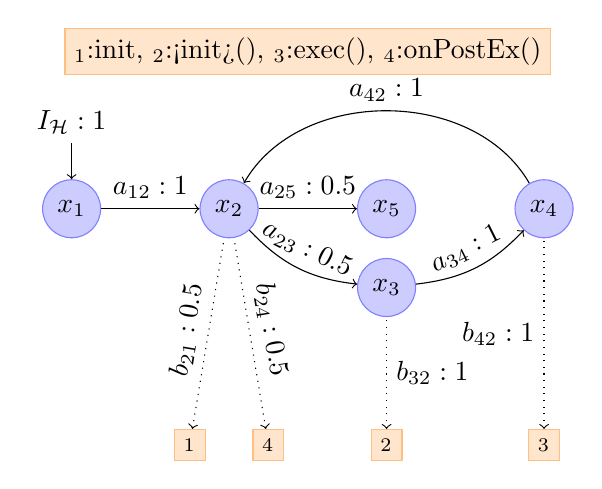
\begin{tikzpicture}[]
% states
\node[hmminitialabove,hmmstate] (x1) at (0,2) {$x_1$};
\node[hmmstate] (x2) at (2,2) {$x_2$};
\node[hmmstate] (x3) at (4,1) {$x_3$};
\node[hmmstate] (x4) at (6,2) {$x_4$};
\node[hmmstate] (x5) at (4,2) {$x_5$};
% transitions
\path[->] (x1) edge node [above] {$a_{12} : 1$} (x2);
\path[->] (x2) edge [bend right = 20] node [above, sloped] {$a_{23} : 0.5$} (x3);
\path[->] (x2) edge node [above] {$a_{25} : 0.5$} (x5);	
\path[->] (x3) edge [bend right = 20] node [above, sloped] {$a_{34} : 1$} (x4);
\path[->] (x4) edge [bend right = 60] node [above] {$a_{42} : 1$} (x2);
    %;
% observations
\node[observation] (o1) at (1.5,-1) {$\absof{\msg}_1$}
	edge [lightedge] node[above,sloped] {$b_{21} : 0.5$} (x2);
\node[observation] (o2) at (2.5,-1) {$\absof{\msg}_4$}
	edge [lightedge] node[above,sloped] {$b_{24} : 0.5$} (x2);
\node[observation] (o3) at (4,-1) {$\absof{\msg}_2$}
	edge [lightedge] node[right] {$b_{32} : 1$} (x3);
\node[observation] (o4) at (6,-1) {$\absof{\msg}_3$}
    edge [lightedge] node[left] {$b_{42} : 1$} (x4);
\node[observation] (legend) at (3,4) { %[above of=x5] {
%	\begin{tabular}{ll}
%		$\obs_1$:&\codej{initial}\\
%		$\obs_2$:&\codej{<init>()}\\
%		$\obs_3$:&\codej{execute()}\\
%		$\obs_4$:&\codej{onPostExecute()}\\
%	\end{tabular}
		$\absof{\msg}_1$:\codej{init},
		$\absof{\msg}_2$:\codej{<init>()},
		$\absof{\msg}_3$:\codej{exec()},
		$\absof{\msg}_4$:\codej{onPostEx()}
%
};
\end{tikzpicture}
} % end subfloat
\subfloat[PFSA with $n = 4$ states]{\label{fig:pfsa-example}
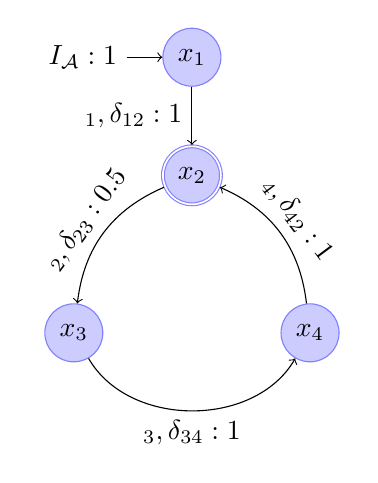
\begin{tikzpicture}[]
% states
\node[pfsainitialleft,hmmstate] (x1) at (2,2.5)    {$x_1$};
\node[hmmstate,pfsafinal] (x2) at (2,1)    {$x_2$};
\node[hmmstate] (x3) at (0.5,-1) {$x_3$};
\node[hmmstate] (x4) at (3.5,-1) {$x_4$};
% transitions
\path[->] (x1) edge node [left] {$\absof{\msg}_1, \delta_{12} : 1$} (x2);
\path[->] (x2) edge [bend right] node [above, sloped] {$\absof{\msg}_2, \delta_{23} : 0.5$} (x3);
\path[->] (x3) edge [bend right = 60] node [below, sloped] {$\absof{\msg}_3, \delta_{34} : 1$} (x4);
\path[->] (x4) edge [bend right] node [above, sloped] {$\absof{\msg}_4, \delta_{42} : 1$} (x2);
    %;
\end{tikzpicture}
} % end subfloat

\subfloat[Lifestate Specification Rules] {
\begin{tabular}{l}
\specAllow{   \codej{init}        }{\codej{<init>()}}\\
\specDisable{ \codej{init}        }{\codej{init}}\\
\specAllow{   \codej{<init>()}    }{\codej{exec()}}\\
\specDisallow{\codej{<init>()}    }{\codej{<init>()}}\\
\specEnable{  \codej{exec()}      }{\codej{onPostEx()}}\\
\specDisallow{\codej{exec()}      }{\codej{exec()}}\\
\specDisallow{\codej{onPostEx()}}{\codej{onPostEx()}}\\
\specAllow{   \codej{onPostEx()}}{\codej{<init>()}}\\
$\ldots$
\end{tabular}
}

\caption{Caption of HMM, PFSA, Specs}
\end{figure*}

\section{OLD Lifestate Specification Section}

\paragraph{Relation to Automaton-Based Specification.}
Fixing the universe of message signatures $\absofset{\MsgSet}$ to be a finite set, we see that that the transition relation $\jstep[\absrules]{\absof{\state}}{\absof{\state}'}$ symbolically describes a particular finite state automaton over the alphabet of transitions $\absofset{\TransSet}$ and potentially $2^{\card{\absofset{\MsgSet}}}$ states.
A state in this automaton corresponds to a particular set of permitted message signatures in a signature state $\absof{\state}\colon \enSigState[ - ][ \absof{\eventmap} ][ \absof{\callinmap} ]$.
However, not every automaton over this alphabet is representable as lifestate rules.
Lifestate rules are ``stateless'' in one respect in that they cannot count previous transitions. For example, for the alphabet $\absofset{\TransSet} = \Set{ \mathtt{a} }$, lifestate rules cannot describe the language $\Set{ \mathtt{a}\mathtt{a} }$.

The reduced expressive power of lifestate rules over automata is potentially beneficial in at least two ways:
\begin{inparaenum}[(1)]
\item enables a more concise representation
\item avoids potentially over-fitting traces.
\end{inparaenum}
The particular stateless semantics of lifestate rules is motivated by the observation that most Android framework messages are stateless in this way.

\paragraph{Probabilistic Lifestate Rules.}

Lifestate rules as defined above are \emph{deterministic} in the sense that on a given forcing $\absforce$, the permitted state $\tuple{ \absof{\eventmap}, \absof{\callinmap} }$ is updated with \emph{all} rules that match $\absforce$ in their antecedent.
Partially stateful lifestate rules can be modeled by extending the rule forms with a probabilistic weight $\weight$ as in $\specEnable[\weight]{\absforce}{\absmsg}$.

The informal semantics of a rule $\absrule\colon \absforce\dashrightarrow_\weight\absmsg$ is that when $\absforce$ is forced, the update of the permitted message signature state according to $\absrule$ happens with probability $\weight$.
This probabilistic extension makes lifestate rules more permissive while still having some restrictions on rule firing (as opposed to a non-deterministic semantics).

Based on the probabilistic semantics, we also define a more permissive, weighted version of trace soundness by applying a particular lower bound weight to the rules in a lifestate specification $\absrules$.
\begin{definition}[$\weight$-Weighted Trace Soundness]\label{def:weighted-trace-soundness}
A signature trace $\abstrace\colon \absof{\trans}_1 \ldots \absof{\trans}_n$ is $\weight$-\emph{sound} with respect to
a lifestate specification $\absof{\directiveset}$ iff there is a sequence of $n$ transitions
\[
\cdots\quad
%\longrightarrow_{\absrules_{i-1}}
{ \enSigState[ \absof{\trans}_i\ldots ][\absof{\eventmap}_i][\absof{\callinmap}_i] }
\longrightarrow_{\absrules_{i}}
{ \enSigState[ \absof{\trans}_{i+1}\ldots ][\absof{\eventmap}_{i+1}][\absof{\callinmap}_{i+1}] }
%\longrightarrow_{\absrules_{i+1}}
\quad\cdots
\]
such that $\absrules_{i} \subseteq \absrules$ for all $1 \leq i < n$ and for each rule $\absrule \in \absrules$, $k_{\absrule} \geq w \cdot n$ where $k_{\absrule}$ is the number of $\absrules_i$'s where $\absrule \in \absrules_i$.
Or informally, the signature trace can be reduced without getting stuck by allowing each rule $\absrule \in \absrules$ to be ignored $< w \cdot n$ times.
\end{definition}

The strict trace soundness (\defref{trace-soundness}) is equivalent to 1-weighted trace soundness. This more general definition is applied in empirically evaluating specification mining algorithms in \secref{evaluation}.

\section{Slicing Stuff}

\begin{figure}\small
\begin{mathpar}
\begin{array}[t]{@{}r@{\;\;}c@{\;\;}l@{\;\;}l@{}}
%\traceslice{\cdot}{\cdot} & : & \multicolumn{2}{l}{\ObsTraceSet \times \ValSet \rightarrow \ObsTraceSet}
%\\
\traceslice{\trans\trace}{\val} & \defeq & \trans(\traceslice{\trace}{\val}) & \text{if $\val \in \EvtArgs(\slicectx)(\trans)$}
\\
\traceslice{\trans\trace}{\val} & \defeq & (\traceslice{\trace}{\val}) & \text{otherwise}
\\
\traceslice{\seq{\enkwInit}\trace}{\val} & \defeq & \traceslice{\trace}{\val}
\\
\traceslice{\cdot}{\val} & \defeq & \cdot
\end{array}

\begin{array}[t]{@{}r@{\;\;}c@{\;\;}l@{}}
%\Args & : & \ObserveSet \rightarrow \powerset(\ValSet)
%\\[0.5ex]
\EvtArgs(\slicectx)(\enEvt{\msg}) & \defeq & \Union_{\msg' \in \slicectx(\msg)} \Args(\msg')
\\
\EvtArgs(\slicectx)(\enObs{\obsty}{\msg}) & \defeq & \Args(\msg) \quad\text{if $\obsty \neq \enkwEvt$}
\end{array}
\end{mathpar}
%
%\begin{array}[t]{@{}r@{\;\;}c@{\;\;}l@{\;\;}l@{}}
%%\Elimci & : & \multicolumn{2}{l}{\ObsTraceSet \rightarrow \ObsTraceSet}
%%\\
%\Elimci(\seq{\enkwInit}) & \defeq & \seq{\enkwInit}
%\\
%\Elimci(\obstrace(\enCi{\msg})\obstrace'(\enRet{\msg})) & \defeq & \Elimci(\obstrace)
%\\
%\Elimci(\obstrace(\enCi{\msg})\obstrace') & \defeq & \Elimci(\obstrace) & \text{if $\enRet{\msg} \notin \obstrace'$}
%\\
%\Elimci(\obstrace(\enDis{\msg})) & \defeq & \Elimci(\obstrace)
%\\
%\Elimci(\obstrace\observe) & \defeq & \Elimci(\obstrace)\observe & \text{otherwise}
%\\[1ex]
%%\Callbacks & : & \multicolumn{2}{l}{\ObsTraceSet \rightarrow \MsgSet \finitemap \powerset(\MsgSet)}
%%\\
%\Callbacks(\seq{\enkwInit}) & \defeq & \empmap
%\\
%\Callbacks(\obstrace(\enEvt{\msg})\obstrace') & \defeq & \Callbacks(\obstrace)\extmap{\msg}{\obstrace'} & \text{if $\enEvt{\msg'} \notin \obstrace'$}
%\\[1ex]
%\traceslice[]{\obstrace}{\val} & \defeq & \traceslice{\obstrace}{\val} & \text{where $\slicectx \defeq \Callbacks(\Elimci(\obstrace))$}
%\end{array}
%
\caption{A callback-driven trace slice $\traceslice{\obstrace}{\val}$ slices a trace $\obstrace$ with respect to a value $\val$ with a context $\slicectx$ about the relation between events and callbacks. The map $\slicectx : \MsgSet \finitemap \finitepowerset(\MsgSet)$ maps event messages to the set of callback messages it invokes so that arguments of an event's callbacks are associated with the initiating event message.}
\label{fig:trace-slice}
\end{figure}

More precisely, we consider a a callback-driven trace slice $\traceslice{\trace}{\val}$ that keeps a transition $\trans$ in $\trace$ if value $\val$ is in the argument set of $\trans$ as shown in \figref{trace-slice}. The map $\slicectx : \MsgSet \finitemap \finitepowerset(\MsgSet)$ provides additional context so that the argument set of event messages can be derived from the argument sets of its callbacks.
We define the callbacks of an event as the set of application methods that it transitively invokes without going through a callin, which we can recover by recording the call tree (e.g., by recording matching call-returns in the trace).

%Because we record the call-returns in the trace, we can recover the callbacks 
%
%This set is defined by eliminating from the observation trace the transitions between matching callins $\enCi{\msg}$ and returns $\enRet{\msg}$ as defined more precisely with $\Elimci : \ObsTraceSet \rightarrow \ObsTraceSet$. In the definition of $\Elimci$, we take the liberty to also treat a sequence as a set.
%Given a observation trace without the transitions between matching callins and returns, an event's callbacks are simply the callbacks between successive events.
%Overall, given an observation trace, the callbacks for each event is computed by $(\Callbacks \circ \Elimci) : \ObsTraceSet \rightarrow \MsgSet \finitemap \finitepowerset(\MsgSet)$.

\section{Eval Stuff}

\begin{figure}\centering
 \includegraphics[width=\linewidth]{new_soundness_1_2}
  \par\includegraphics[width=\linewidth]{new_soundness_1_1}
\caption{Sufficiency measures the fraction of $\weight$-sound traces of a given testing set with respect to a given specification (higher is better).
For each training set for a framework type, we measure sufficiency for each learned specification on the corresponding testing set.
The y-axis shows the average sufficiency measure over the testing sets (from 5-fold cross validation) for each framework type grouped by learning method. The rightmost bar in each group shows the average over the four framework types. We consider two soundness weights: $w = 1$ corresponding to strict soundness and $w = 1 / 2$ corresponding to each rule applying at least half of the time when matched (see \defref{weighted-trace-soundness}).}
%\caption{The geometric mean of the sufficiency ratio for all of the training and test sets is shown on the Y axis. The X axis shows the learning methods, in the case of \sharpsat there is also a threshold. The w is the weighted trace soundness as defined in 3.}
 \label{fig:soundnessres-appendix}
\end{figure}

\section{Other Stuff}
%
\newsavebox{\SBoxFeedRemoverProjectedAll}
\begin{lrbox}{\SBoxFeedRemoverProjectedAll}\small
\begin{tabular*}{\linewidth}{@{}l@{}}
\fbox{\codej{a:Activity}}
\\
\begin{lstlisting}[language=Java,alsolanguage=exthighlighting]
|evt:Create|$\frameop$Activity.onCreate()
\end{lstlisting}
\\\\[-1ex]
\fbox{\codej{t1:AsyncTask}}
\\
%|evt:Execute|$\frameop$AsyncTask.doInBackground()#\textrm{ on thread 1}#
\begin{lstlisting}[language=Java,alsolanguage=exthighlighting]
AsyncTask.<init>()
AsyncTask.execute()
|evt:PostExecute|$\frameop$AsyncTask.|cb:onPostExecute|()
\end{lstlisting}
\\\\[-1ex]
\fbox{\codej{b:Button}}
\\
\begin{lstlisting}[language=Java,alsolanguage=exthighlighting]
Button.setOnClickListener(OnClickListener)
|evt:Click|$\frameop$OnClickListener.onClick(Button)
Button.setEnabled(false)
Button.setEnabled(true)
\end{lstlisting}
\\\\[-1ex]
\fbox{\codej{l:OnClickListener}}
\\
\begin{lstlisting}[language=Java,alsolanguage=exthighlighting]
Button.setOnClickListener(OnClickListener)
|evt:Click|$\frameop$OnClickListener.onClick(Button)
\end{lstlisting}
\\\\[-1ex]
\fbox{\codej{t2:AsyncTask}}
\\
\begin{lstlisting}[language=Java,alsolanguage=exthighlighting]
AsyncTask.<init>()
\end{lstlisting}
\end{tabular*}
\end{lrbox}

%%% Local Variables:
%%% mode: latex
%%% TeX-master: t
%%% End:
